\documentclass{ustbthesis}

\usepackage[backend=biber,
style=gb7714-2015,
    sortcites=true,autocite=inline,autopunct=true,hyperref=true,
    natbib
    ]{biblatex}

\hypersetup{hidelinks,colorlinks=false,citecolor=black}
\addbibresource{myrefs.bib}

\usepackage{tabularx}
\usepackage{amsmath}
\usepackage{amssymb}
\usepackage[labelfont=bf,textfont=bf,font=small]{subfig}
\newcommand{\figref}[1]{~\ref{#1}~}
\newcommand{\tabref}[1]{~\ref{#1}~}

\newcolumntype{P}[1]{>{\centering\arraybackslash}p{#1}}
%%%%%%%%%%%%%%%%%%%%%%%%%%%封面信息%%%%%%%%%%%%%%%%%%%%%%%%%%%%%%%%%%
%% 作者
\Author{梁 辰}
\EnglishAuthor{Liang Chen}
%% 标题
\Title{面向反无人机场景的无人机识别与定位系统设计与实现}
\EnglishTitle{Design and Implementation of a Drone Recognition and Localization System for Counter-UAV Scenarios}
%% 日期
\Date{2026年 11月 20日}
\EnglishDate{Nov, 2026}
%% 学院
\College{数理学院}
\EnglishCollege{School of Mathematics and Physics}
%% 地址
\Address{海淀区学院路30号}
\EnglishAddress{30 Xueyuan Road，Haidian District}
%%培养单位（所在单位、学位授予单位）%%
\Affiliation{北京科技大学}
\EnglishAffiliation{University of Science and Technology Beijing}
%% 邮编
\Postcode{100083}
%% 城市
\City{北京}
\EnglishCity{Beijing}
%% 国家
\Country{中国}
\EnglishCountry{P.R.CHINA}
%%学号%%
\StudentCode{M202640106}
%%专业%%
\Major{软件工程}
\EnglishMajor{Software Engineering}
%%研究方向%%
\Direction{计算机视觉方向}
\EnglishDirection{Computer Vision}
%%导师%%
\Supervisor{段世红}
\EnglishSupervisor{Shihong Duan}

\DegreeType{学术型}
\EnglishDegreeType{Science}

%%中图分类号%%
\CLCNumber{TP391}
%%UDC分类号%%
\UDCNumber{004.8}
%%学校代码%%
\UniversityCode{10008}
\UniversityLogoFile{images/ustb.png}
%% 密级
\SecurityLevel{公开}
%% 提交日期
\SubmissionDate{2026年 11月 20日}
\EnglishSubmissionDate{Nov, 2026}
%%%%%%%%%%%%%%%%%%%%%%%%%%%封面信息%%%%%%%%%%%%%%%%%%%%%%%%%%%%%%%%%%
\begin{document}

\TitlePage

\SecondPage

\ThirdPage

\pagestyle{fancy}

%% 中英文摘要
%% 中英文摘要
\begin{ChineseAbstract}

随着低空禁忌的快速发展，微型无人机在救援、航拍、物流、巡检等多领域广泛应用，但"黑飞""乱飞"等违规飞行事件也随之增多，对机场，军区等保密单位构成了威胁。这一问题已成为反无人机领域待解决的关键问题。雷达，声学，光学，视觉等光学视觉方案具有成本低，部署灵活，可直观确认目标等优势，但同时也面临这两个突出的问题，第一个问题较远距离目标在图像中成像过小，约几十个像素，属于小目标检测问题；第二个问题是在真实的场景环境中，树木、建筑等障碍物随处可见，检测数据中断较为频繁，难以形成连续，持久，可用的航迹。

针对以上问题，本文设计并实现了一个面向反无人机场景的无人机识别与定位系统。在这个系统中，单目可见相机是唯一的视觉传感器，通过“检测-跟踪-定位-显示”这一流程，主要工作包含了以下五个方面。

（1）面向小目标检测搭建模型。该模型以YOLOv8n为基础，在特征金字塔中增加stride=4的P2高分辨率检测头，并且在C2f模块中嵌入EMA搞笑多尺度注意力机制，结合成YOLOv8n-P2-EMA模型。随后将Det-Fly数据集划分为训练集与验证集，避免同一序列帧同时出现在训练和验证中，造成数据泄露。四组消融实验表明：YOLOv8n、+P2、+EMA、+P2+EMA的mAP50分别为 81.3\%、82.3\%、76.2\% 与 83.5\%，AP\_small 分别为 6.1\%、8.3\%、4.1\% 与 9.8\%，推理速度分别为 123、90、101 与 98\,fps。本文模型以 2.94\,M 参数量取得最优综合指标，AP\_small 相对基线提升 60.7\%，并可满足 30\,fps 实时处理需求。

（2）揭示了仿真环境下检测死区的形成机理。在 PX4+jMAVSim 测试中发现，未微调模型在 3--6\,m 近距离段检出率接近 0，在 9\,m 以上远距离段亦无法稳定锁定，有效工作窗口仅 7--9\,m。通过对 2228 帧录像与真值几何的逐帧审计，排除了"俯视视角导致失效"的假设，确认死区的决定因素是目标在图像中的尺度：近距离大尺度样本超出 Det-Fly 的远距小目标分布，属于分布外（OOD）输入；远距离样本则低于初锁门限。

（3）提出了仿真域微调方法并完成自动标注数据构建。利用 jMAVSim 护航相机始终注视目标机的特性，将目标框中心约束在光轴附近，再由真值距离与等效尺寸反算框高，实现零人工标注的 450 帧仿真数据采集；按距离分层覆盖 3--6\,m、6--7\,m、7--9\,m 与 9--12\,m 四个区间。以 20 轮、学习率 0.001、关闭 Mosaic 的方式微调后，3--10\,m 全距离段检出率提升至 100\%，置信度中位数 0.867，检测死区被完全消除。

（4）设计了三态跟踪状态机与单目定位方法。状态机包含 SEARCH、LOCKED 与 COAST 三种状态，采用"0.25 维持门限 + 0.55 初锁门限"的双门限策略抑制误锁，采用 140\,px 空间门限的最近邻匹配抑制身份跳变，采用 1.0\,s 卡尔曼预测维持抑制短时遮挡中断。定位环节由检测框中心直接解算方位角与俯仰角，由框高与等效尺寸解算距离，并以六维状态的自适应卡尔曼滤波（Sage-Husa）平滑三维位置与速度。仿真闭环实验表明，微调后单帧测距 RMSE 为 0.26\,m、AKF 稳态中位误差 0.13\,m、1\,s 距离预测 ADE 中位 0.26\,m、方位角误差中位 0.05\textdegree；实拍视频中 AKF 相对单帧测距 RMSE 降低 32\%，抖动降低 33\%。

（5）完成了系统集成与自动化验证。系统采用"算法端—显示端"双进程架构，算法进程通过 TCP 接收 720p@30fps 视频帧、通过 UDP 接收 50\,Hz 真值，并以 UDP/JSON 向显示端输出结构化结果；基于 PySide6 构建三页签监视大屏，包含卫星地图态势、光电画面、距离与方位仪表、威胁分级、CSV 记录与参数持久化等功能。设计并执行了 14 个自动化用例，覆盖基线检测、真实场景、门限扫描、尺寸敏感、TCP 遮挡与摄像头输入，13 例完成、6 例判定通过、0 例失败，验证了完整链路的正确性与鲁棒性。

最后，本文将所提方法应用于改造后的 jMAVSim 城市巡游场景，实现了目标机主动飞行、护航相机被动尾随的编队巡游，并通过段内加减速与瞄准点滞后使画面呈现真实的追踪感，为后续外场试验与多传感器融合提供了可复现的实验平台。

\textbf{关键词：}反无人机；小目标检测；YOLOv8；P2 检测头；EMA 注意力；卡尔曼滤波；单目测距；仿真域微调

\end{ChineseAbstract}

\begin{EnglishAbstract}

With the rapid development of the low-altitude economy, micro unmanned aerial vehicles (UAVs) have been widely used in many fields such as rescue, aerial photography, logistics, and inspection. However, illegal and irregular flight events such as ``black flights'' and ``chaotic flights'' have also increased, posing threats to airports, military regions, and other confidential units. This problem has become a key issue to be solved in the counter-UAV field. Radar, acoustic, optical, and vision-based solutions have advantages such as low cost, flexible deployment, and intuitive target confirmation, but they also face two prominent problems. The first problem is that distant targets are imaged too small in images, about tens of pixels, which belongs to small-object detection. The second problem is that in real scenarios, obstacles such as trees and buildings are ubiquitous, and detection data interruptions are frequent, making it difficult to form continuous, persistent, and usable tracks.

To address the above problems, this paper designs and implements a UAV identification and localization system for counter-UAV scenarios. In this system, a monocular visible-light camera is the only visual sensor. Through the pipeline of ``detection--tracking--localization--display'', the main work includes the following five aspects.

(1) A model for small-object detection is built. The model is based on YOLOv8n, adds a P2 high-resolution detection head with stride=4 to the feature pyramid, and embeds an Efficient Multi-Scale Attention (EMA) mechanism into the C2f module, forming the YOLOv8n-P2-EMA model. Then the Det-Fly dataset is divided into training and validation sets to avoid the same sequence frames appearing in both training and validation and causing data leakage. Four ablation experiments show that the mAP50 of YOLOv8n, +P2, +EMA, and +P2+EMA are 81.3\%, 82.3\%, 76.2\%, and 83.5\%, respectively; AP\_small are 6.1\%, 8.3\%, 4.1\%, and 9.8\%, respectively; and the inference speeds are 123, 90, 101, and 98\,fps, respectively. The proposed model achieves the best overall performance with 2.94\,M parameters; AP\_small is improved by 60.7\% relative to the baseline, and it can meet the 30\,fps real-time processing requirement.

(2) The formation mechanism of the detection dead zone in the simulation environment is revealed. In PX4+jMAVSim tests, it is found that the detection rate of the model without fine-tuning is close to 0 in the near range of 3--6\,m, and it cannot stably lock in the far range above 9\,m; the effective working window is only 7--9\,m. Through frame-by-frame audit of 2228 frames of video and ground-truth geometry, the hypothesis that ``the top-down view causes failure'' is ruled out, and it is confirmed that the decisive factor of the dead zone is the scale of the target in the image: near-range large-scale samples exceed the far-range small-target distribution of Det-Fly and belong to out-of-distribution (OOD) inputs; far-range samples are below the initial locking threshold.

(3) A simulation-domain fine-tuning method is proposed and automatic annotation data construction is completed. Taking advantage of the characteristic that the jMAVSim escort camera always looks at the target UAV, the center of the target box is constrained near the optical axis, and then the box height is back-calculated from the ground-truth distance and equivalent size, realizing zero-manual-annotation collection of 450 frames of simulation data; the data are stratified by distance and cover four intervals: 3--6\,m, 6--7\,m, 7--9\,m, and 9--12\,m. After fine-tuning for 20 epochs with a learning rate of 0.001 and Mosaic disabled, the detection rate over the full range of 3--10\,m is increased to 100\%, the median confidence is 0.867, and the detection dead zone is completely eliminated.

(4) A three-state tracking state machine and a monocular localization method are designed. The state machine contains three states: SEARCH, LOCKED, and COAST. A dual-threshold strategy of ``0.25 maintenance threshold + 0.55 initial locking threshold'' is used to suppress false locking; nearest-neighbor matching with a 140\,px spatial threshold is used to suppress identity switching; and 1.0\,s Kalman prediction maintenance is used to suppress short-term occlusion interruptions. In the localization stage, the azimuth and elevation angles are directly solved from the center of the detection box, the distance is solved from the box height and equivalent size, and a six-dimensional state adaptive Kalman filter (Sage-Husa) is used to smooth the 3D position and velocity. Simulation closed-loop experiments show that after fine-tuning, the single-frame ranging RMSE is 0.26\,m, the AKF steady-state median error is 0.13\,m, the median ADE of 1\,s distance prediction is 0.26\,m, and the median azimuth error is 0.05\textdegree; in real captured videos, the AKF reduces the RMSE by 32\% and the jitter by 33\% compared with single-frame ranging.

(5) System integration and automated verification are completed. The system adopts a dual-process architecture of ``algorithm side--display side''. The algorithm process receives 720p@30\,fps video frames via TCP and 50\,Hz ground truth via UDP, and outputs structured results to the display side via UDP/JSON; a three-tab monitoring dashboard is built based on PySide6, including satellite map situation, electro-optical imagery, distance and azimuth gauges, threat grading, CSV logging, and parameter persistence. Fourteen automated test cases are designed and executed, covering baseline detection, real scenes, threshold sweeping, size sensitivity, TCP occlusion, and camera input. Thirteen cases are completed, six are judged as passed, and zero cases failed, verifying the correctness and robustness of the complete pipeline.

Finally, the proposed method is applied to a modified jMAVSim urban patrol scene, realizing a formation patrol in which the target UAV flies actively and the escort camera passively tails it. Through intra-segment acceleration/deceleration and aiming-point lag, the image presents a realistic tracking feel, providing a reproducible experimental platform for subsequent field tests and multi-sensor fusion.

\textbf{Keywords:} counter-UAV; small object detection; YOLOv8; P2 detection head; EMA attention; Kalman filter; monocular ranging; simulation-domain fine-tuning

\end{EnglishAbstract}

%% 目录
\tableofcontents

\mainmatter
\pagenumbering{arabic}\setcounter{page}{1}
\pagestyle{fancy}

%% 第一章 绪论
\chapter{绪论}

\section{研究背景}

\subsection{低空经济发展与无人机规模化应用}

过去十年间，微机电系统、飞控算法、电池与无线通信等技术的成熟，使多旋翼无人机从专业航拍设备迅速演变为大众消费品。以 DJI、道通、零度等厂商为代表的企业将整机价格下探至数千元量级，起飞重量低于 250\,g 的微型无人机甚至可以免注册购买。与之相伴的是低空空域活动密度的快速上升：航拍测绘、电力巡检、农林植保、快递物流、应急救援、灯光表演等应用场景不断扩展，城市低空正在形成一个新的经济形态，即通常所说的"低空经济"。

低空经济的繁荣带来了空域治理的新问题。一方面，无人机的合法运行需要飞行计划报备、空域申请、实名登记与实时监管；另一方面，无人机的获取门槛极低、操控简单、体积小巧，使得"黑飞"（未经许可的飞行）、"乱飞"（违反禁飞区或高度限制的飞行）以及恶意入侵难以通过传统手段有效遏制。近年来，国内外多次出现无人机闯入机场净空区导致航班大面积延误、无人机近距离拍摄军事设施或敏感区域、无人机携带危险载荷飞越人群等事件。这些事件表明，低空安全已经从理论风险转变为现实威胁，反无人机（Counter-UAV，C-UAV）技术因此成为学术界、产业界与监管部门共同关注的热点。

\subsection{反无人机系统的典型环节与技术路线}

一个完整的反无人机系统通常可以划分为"探测—识别—跟踪—定位—处置"五个环节\cite{radar_cuav,fusion_cuav}。探测环节负责发现空域中是否存在可疑目标；识别环节负责判定目标类型（无人机、鸟类、风筝、飞机等）；跟踪环节负责在时间序列上维持对同一目标的连续观测；定位环节负责给出目标相对观测平台或地理坐标系的位置；处置环节则根据威胁等级采取告警、干扰、诱骗或拦截等措施。其中，探测、跟踪与定位构成了整个系统的信息基础，其性能直接决定了后续处置是否可行。

按照所使用的物理媒介，现有探测手段可以分为雷达、射频、声学、光学以及多传感器融合五类，表~\ref{tab:sensing_compare} 对它们进行了对比。

\begin{table}[htbp]
\centering
\caption{典型反无人机探测手段对比}
\label{tab:sensing_compare}
\small
\begin{tabularx}{\textwidth}{P{2.0cm}P{2.2cm}P{2.5cm}P{2.8cm}X}
\toprule
\textbf{手段} & \textbf{作用距离} & \textbf{优势} & \textbf{局限} & \textbf{适用场景} \\
\midrule
雷达 & 数百米至数公里 & 全天候、测距测速直接 & 小型目标雷达散射截面积小、设备昂贵、需频率许可 & 机场、边境、要地远程预警 \\
射频侦测 & 数百米至数公里 & 被动工作、可识别型号 & 目标静默时失效、无法定位非合作目标 & 城市频谱监测 \\
声学探测 & 数十米至数百米 & 成本低、可被动布设 & 易受环境噪声干扰、作用距离短 & 楼宇近程补盲 \\
光学视觉 & 数十米至数百米 & 成本低、部署灵活、可直观确认 & 受光照与天气影响、小目标检出难、遮挡敏感 & 近程确认、跟踪与取证 \\
多传感器融合 & 视配置而定 & 互补性强、可靠性高 & 系统复杂、时空配准与数据融合难度大 & 高等级防护系统 \\
\bottomrule
\end{tabularx}
\end{table}

由表可见，雷达适合远距离预警，但对低慢小目标的探测能力有限，且设备成本与部署门槛较高\cite{radar_cuav}；射频侦测属于被动手段，一旦目标进入静默状态便完全失效\cite{rf_drone}；声学探测成本低廉，但作用距离通常只有百米量级，且在城市噪声环境下虚警率较高\cite{acoustic_drone}；多传感器融合虽然性能最好，却需要解决异构传感器的时空配准、数据关联与决策融合等一系列工程问题\cite{fusion_cuav,rf_remoteid}。相比之下，光学视觉方案只需要一台普通可见光相机与一台计算设备，成本低、部署灵活，并且能够提供目标的外观证据，便于操作员人工复核，因而成为近程反无人机系统中不可替代的组成部分\cite{optical_cuav}。

\subsection{光学视觉方案面临的核心困难}

尽管优势明显，光学视觉方案在真实反无人机场景中仍面临两方面突出困难。

第一，\textbf{小目标检测难}。反无人机系统追求"早发现"，而越早发现意味着目标越远、成像越小。在 1280$\times$720 分辨率的图像中，100\,m 外的微型无人机往往只占十几个像素，即使在大倍率长焦镜头下也可能不足 50 像素。通用目标检测模型在 COCO 等以中大型目标为主的数据集上训练，其特征金字塔的最深层对应 32 倍下采样，微小目标在深层特征图上仅剩不到一个像素，响应极弱。Det-Fly 等无人机检测数据集的统计也表明，目标框面积中位数不足画面面积的 0.06\%，99\% 以上的目标框面积小于画面的 1\%。如何在保持实时性的前提下提升小目标召回率，是检测环节的首要问题。

第二，\textbf{遮挡与抖动导致跟踪中断}。真实低空空域中充满树木、建筑、电线、广告牌等遮挡物，目标在飞行过程中频繁被短时遮挡。若系统以"每帧检测成功"为输出前提，则遮挡发生时输出会瞬间消失，航迹断裂、告警闪烁，操作员无法判断目标是暂时被遮挡还是已经飞离。此外，检测框本身存在像素级抖动，直接由框尺寸反算距离会产生米级跳变。如何在检测缺失时维持航迹、在检测存在时平滑输出，是跟踪与定位环节的核心问题。

除上述两点之外，工程落地还面临第三个困难：\textbf{仿真与真实域之间的差异}。出于成本与空域限制，算法开发通常先在仿真环境中完成闭环验证，再迁移到真实设备。然而仿真渲染的光照、纹理、边缘与真实相机存在显著差异，在真实数据上训练的模型直接用于仿真画面时可能出现严重的性能退化。本文在实验初期即观察到了这一现象，并将其作为一项专门的研究内容。

\section{研究意义}

\subsection{理论意义}

本文的研究意义首先体现在对小目标检测机理的补充上。现有工作大多从"增加检测层""引入注意力""改进损失函数"等角度提升指标，但对改进为何有效、在何种条件下失效缺乏统一解释。本文通过四组消融实验，将 P2 检测头的作用归结为"保留浅层空间分辨率"，将 EMA 的作用归结为"在通道与空间两个维度重加权"，并通过 +EMA 单独失效、+P2+EMA 联合有效的现象，说明二者存在"看清"与"认准"的互补关系。这一解释对小目标检测的网络设计具有一般性参考价值。

其次，本文对仿真域检测死区的机理分析具有方法论意义。面对"模型在仿真中失效"这一现象，容易产生的第一反应是"视角不合适"或"渲染质量差"。本文通过真值几何审计与距离分层统计，定量排除了视角假设，将原因定位为目标尺度分布偏移，并进一步用仿真域微调实验验证了该解释。这种"现象—假设—证伪—验证"的分析路径，比单纯报告指标更有助于理解域偏移的本质。

最后，本文将三态状态机、单目测距与自适应滤波整合为一条可运行的完整链路，并在统一的时间基准下评估检测、跟踪与定位的耦合性能，为反无人机视觉系统提供了一套可复现的工程范式。

\subsection{工程意义}

从工程角度看，本文系统具有以下价值。其一，硬件门槛低。系统仅依赖单目可见光相机与一台带 GPU 的普通计算机，不需要激光雷达、毫米波雷达或高精度惯导，便于在园区、楼宇、临时活动现场快速部署。其二，链路完整。系统不仅输出检测框，还输出目标距离、方位角、俯仰角、速度、威胁等级以及地理坐标，可直接对接上级指挥系统。其三，可测试性强。本文设计了 14 个自动化用例与统一的 CSV 记录格式，能够在无人值守条件下完成回归测试，为后续迭代提供量化基线。其四，可复现性强。仿真环境、数据采集脚本、自动标注流程与训练配置均已固化，研究者和工程师可以在相同条件下复现本文的全部实验。

\section{国内外研究现状}

\subsection{通用目标检测算法的发展}

目标检测算法的发展大致经历了三个阶段。第一阶段以手工特征与分类器组合为主，代表性方法是 HOG+SVM 与可变形部件模型（DPM），其检测精度依赖人工设计的特征，泛化能力有限。第二阶段以深度卷积网络为特征提取器，形成了两阶段与单阶段两条技术路线。两阶段方法以 Faster R-CNN\cite{faster_rcnn} 为代表，先由区域建议网络（RPN）生成候选框，再对候选框进行分类与回归，精度较高但速度较慢；单阶段方法以 SSD\cite{ssd} 与 YOLO 系列\cite{yolov1,yolov5,yolov8} 为代表，直接在特征图上预测类别与边框，速度优势明显。第三阶段以 Transformer 架构为代表，RT-DETR\cite{rt_detr} 通过编码器—解码器结构与集合预测损失摆脱了锚框与非极大值抑制，在精度上接近甚至超过同期 YOLO，但计算量与部署复杂度更高。

在工程实践中，YOLO 系列因其"精度—速度—易用性"的平衡而成为主流选择。YOLOv5\cite{yolov5} 确立了以 CSPDarknet 为骨干、PANet 为颈部、解耦头为头部的结构；YOLOv8\cite{yolov8} 在此基础上引入 C2f 模块与更灵活的任务对齐分配策略，并提供 n/s/m/l/x 五种规模。本文选择 YOLOv8n 作为基础模型，主要基于三点考虑：参数量约 3\,M，便于与桌面应用集成；在 RTX 4060 级别 GPU 上批量推理可达 100\,fps 以上；Ultralytics 提供了成熟的训练、验证与导出接口，便于复现实验。

\subsection{无人机小目标检测研究现状}

针对无人机小目标检测，现有研究大致可以分为四类。

第一类是\textbf{增加高分辨率检测层}。标准 YOLO 的最浅检测层为 P3（stride=8），对于十几个像素的目标仍显不足。SOD-YOLOv8\cite{sod_yolov8} 在 YOLOv8 中增加更高分辨率的检测分支，并配合特征融合，提升了交通场景中小目标的召回率。本文将这一思想应用于无人机场景，增加 stride=4 的 P2 检测头，使 40\,px 的目标在特征图上仍占据 10 个网格单元，而不是 5 个。

第二类是\textbf{引入注意力机制}。CBAM\cite{cbam} 通过通道注意力与空间注意力串联，增强目标区域响应；EMA\cite{ema} 则采用分组并行与跨空间学习，在较低计算开销下同时建模通道与空间关系。YOLOv8-MPEB\cite{yolov8_mpeb} 将骨干替换为 MobileNetV3 并引入高效多尺度注意力，实现轻量化无人机检测。MSDF-Net\cite{msdf_net} 结合可变形卷积与高分辨率特征增强，在林业病害检测中验证了跨版本特征增强的有效性。

第三类是\textbf{改进损失函数与标签分配}。小目标对定位误差极为敏感，IoU 系列损失在目标框很小时梯度不稳定。SIoU\cite{seiou} 引入角度代价，使回归方向更明确；Wise-IoU 通过动态聚焦机制降低低质量样本的梯度权重。本文在训练中沿用 YOLOv8 默认的 TaskAlignedAssigner 与 CIoU 损失，未对损失函数做额外改动，以保持与基线模型的可比性。

第四类是\textbf{数据集与评测协议}。Det-Fly\cite{detfly} 是目前公开的较大规模无人机检测数据集之一，包含多种背景、多种机型与多种飞行状态。UAVDT\cite{uavdt} 则面向城市交通场景中的无人机跟踪。Kurmashev 等人\cite{yolov12_adbc} 系统比较了不同 YOLO 版本在无人机检测任务上的表现，指出模型规模、输入分辨率与数据分布对结果的影响远大于网络结构的细微差异。这一结论提醒我们：在报告指标时必须明确数据划分与评测口径，否则容易得出误导性结论。

\subsection{反无人机系统研究现状}

完整的反无人机系统研究主要集中在三个方向。

其一是\textbf{多传感器融合}。文献\cite{rf_remoteid} 提出融合射频、光学与雷达的多模态框架，利用 Remote ID 广播信号进行身份识别，利用视觉进行确认，利用雷达进行测距；文献\cite{fusion_cuav} 对现有反无人机方法与基准进行了系统综述，指出单一传感器在复杂环境下均存在盲区，融合是提升可靠性的必然选择。

其二是\textbf{射频与声学探测}。文献\cite{rf_drone} 利用无人机图传与遥控链路的射频特征实现检测与跟踪，能够在目标静默前提供较远距离的预警；文献\cite{acoustic_drone} 利用 MEMS 麦克风阵列与机器学习实现被动声学定位，成本极低但作用距离受限。

其三是\textbf{视觉检测与跟踪}。文献\cite{optical_cuav} 对比了 YOLO 与 Faster R-CNN 在监控视频中的微型无人机检测性能，发现单阶段模型在速度上具有明显优势，而两阶段模型在极小目标上略优。总体来看，现有工作多聚焦于单一算法环节的指标提升，面向完整链路、可实际运行、具备可视化界面的系统级开源实现相对缺乏，这正是本文的切入点。

\subsection{单目定位与目标跟踪研究现状}

在定位方面，单目视觉测距通常有三类方法。第一类基于已知目标尺寸，利用相似三角形关系由框高或框宽反算距离，实现简单但对目标尺寸先验依赖强；第二类基于地面平面假设，利用相机高度与像平面几何关系解算目标落点，适用于地面目标；第三类基于多帧运动，通过特征点跟踪与三角化恢复深度，计算量大且对纹理敏感。本文的目标是空中无人机，不具备地面平面约束，且外观尺寸相对稳定，因此选择第一类方法，并通过仿真域标定获得等效尺寸。

在跟踪方面，SORT\cite{sort} 用卡尔曼滤波预测目标位置、用匈牙利算法关联检测框，奠定了多目标跟踪的基本框架；DeepSORT\cite{deepsort} 引入外观特征以降低身份切换。本文面向单目标跟踪场景，不需要外观重识别，但借鉴了"预测—关联—更新"的思想，并将关联失败时的处理显式建模为 COAST 状态。卡尔曼滤波\cite{kalman} 是最优线性估计的经典方法，但其量测噪声协方差需要预先设定。Sage-Husa 自适应滤波\cite{sagehusa} 通过残差在线估计噪声统计特性，能够在量测质量变化时自动调整滤波增益，本文采用该思路构建自适应卡尔曼滤波器（AKF）。

\subsection{仿真验证与域适应研究现状}

受空域管制与成本限制，无人机算法的早期验证通常依赖仿真。PX4\cite{px4} 是应用最广泛的开源飞控固件，支持 SITL（Software In The Loop）模式；jMAVSim\cite{jmavsim} 是其自带的轻量级三维仿真器，基于 Java3D 构建，能够以较低的资源开销模拟多旋翼动力学与相机视图。Gazebo 与 AirSim 提供更逼真的渲染，但对显卡与计算资源要求更高。本文选择 jMAVSim，主要原因是其启动快、可定制性强，便于通过 Java 源码改造注入目标机、相机与真值广播。

仿真到真实的域差异（sim-to-real gap）是近年来的研究热点。常见做法包括风格迁移、域随机化与目标域微调。风格迁移通过生成对抗网络将仿真图像转换为真实风格，但可能引入伪影；域随机化在训练时随机改变光照、纹理与噪声，提升模型鲁棒性，但需要大量训练资源；目标域微调则直接用少量目标域数据调整模型参数，简单有效。本文采用目标域微调路线，并针对仿真环境设计了零人工标注的采集流程，以较低成本消除了检测死区。

\section{现有方案的不足与本文切入点}

综合上述分析，现有方案存在以下不足。

（1）\textbf{小目标改进缺乏机理层面的解释}。多数工作只报告 mAP 提升，未说明改进在何种尺度、何种背景下起作用，也未讨论单独使用某一模块时可能出现的性能下降。本文通过消融实验与特征尺度分析，给出 P2 与 EMA 互补的解释。

（2）\textbf{仿真验证中的性能退化被忽视}。不少工作在仿真环境中直接使用真实数据训练的模型，遇到性能下降时归因于"渲染不真实"，缺少定量分析。本文通过逐帧真值审计定位死区成因，并用微调实验闭环验证。

（3）\textbf{跟踪与定位耦合不足}。检测、跟踪、测距往往被分别评估，缺少在统一时间基准下的端到端指标。本文在仿真闭环中以 50\,Hz 真值为基准，同时评估检出率、测距误差、角度误差与预测误差。

（4）\textbf{系统级实现与可复现性不足}。许多研究停留在脚本与 notebooks 层面，缺少可视化界面、参数管理、日志记录与自动化测试。本文构建了完整的桌面系统与测试框架，并将全部配置固化。

基于以上分析，本文的切入点可以概括为：\textbf{以单目可见光相机为传感器，以改进的 YOLOv8n 为检测前端，以三态状态机为跟踪骨架，以自适应卡尔曼滤波为定位核心，以仿真闭环为验证平台，构建一套端到端可运行、可测试、可复现的反无人机识别与定位系统}。

\section{本文主要研究内容}

本文的主要研究内容包括以下五个方面。

（1）\textbf{小目标检测模型改进与消融分析}。在 YOLOv8n 上增加 P2 检测头与 EMA 注意力，构建四种模型配置，在 Det-Fly 数据集上按序列划分训练/验证集，完成消融实验，并从特征分辨率与注意力重加权两个角度解释结果。

（2）\textbf{数据集构建与数据工程}。完成 Det-Fly 数据格式转换、序列级划分与统计分析；采集自建 AprilTag 标定数据用于相机内参标定与定位精度评估；构建 450 帧仿真自动标注数据集，用于仿真域微调。

（3）\textbf{三态跟踪状态机设计}。针对误检、跳变与遮挡三个问题，设计 SEARCH/LOCKED/COAST 状态机，给出双门限、空间门限与超时参数的选择依据，并通过遮挡用例验证 COAST 的航迹保持效果。

（4）\textbf{单目定位与自适应滤波}。建立针孔相机模型，推导方位角、俯仰角与距离的解算公式，分析测距误差随距离与框高误差的传播规律；设计六维状态自适应卡尔曼滤波器，给出预测步与更新步的完整推导，并通过仿真与实拍数据评估平滑与预测性能。

（5）\textbf{仿真闭环与系统实现}。改造 PX4+jMAVSim 闭环，注入脚本目标机、护航相机、真值广播与离屏帧流；分析并消除检测死区；基于 PySide6 实现三页签监视大屏；设计 14 个自动化用例完成回归测试；进一步实现目标机主动飞行、相机被动尾随的编队巡游与加减速行为。

\section{论文组织结构}

本文共分十章，各章内容安排如下。

第一章为绪论。介绍研究背景、反无人机系统的技术路线、光学视觉方案的核心困难，综述国内外研究现状，分析现有方案的不足，并给出本文的研究内容与组织结构。

第二章为相关理论与关键技术。介绍卷积神经网络与目标检测的基本原理、YOLOv8 的网络结构、注意力机制、卡尔曼滤波、针孔相机模型、PX4 与 jMAVSim 仿真框架、PySide6 与网络通信等本文所依赖的理论与技术基础。

第三章为数据集构建与数据工程。介绍 Det-Fly 数据集的来源、格式、统计特性与序列级划分方法；介绍自建 AprilTag 数据集的采集与标定流程；介绍仿真自动标注数据集的构建方法；讨论数据增强与评测口径。

第四章为检测模型改进与消融实验。详细阐述 P2 检测头与 EMA 注意力的设计，给出网络结构、计算量与感受野分析；介绍训练配置与损失函数；给出四组消融实验结果，并从尺度分布、注意力响应与参数效率三个角度解释结果；最后讨论模型的有效工作范围。

第五章为三态跟踪状态机。分析直接使用检测输出导致的误检、跳变与遮挡问题；给出状态定义、转移条件与参数选择；详细描述 SEARCH、LOCKED、COAST 三个状态的处理流程；给出伪代码与复杂度分析；通过遮挡用例验证航迹保持效果。

第六章为单目定位与自适应卡尔曼滤波。建立相机坐标系与像素坐标系的映射关系；推导方位角、俯仰角与距离的解算公式；分析测距误差传播；设计六维状态自适应卡尔曼滤波器，推导预测与更新过程；给出角度解算的两种实现及其对比；最后通过仿真与实拍数据评估定位精度。

第七章为仿真闭环系统与域微调。介绍 PX4 SITL 与 jMAVSim 的架构；详细说明本文对 jMAVSim 的改造，包括脚本目标机、护航相机、真值广播、离屏帧流与场景构建；描述检测死区的发现过程与机理分析；给出自动标注数据采集、距离分层采样与微调配置；展示微调前后的对比结果；介绍编队巡游与尾随相机的实现。

第八章为系统设计与实现。给出需求分析、总体架构与双进程通信协议；介绍算法端的模块划分、状态机实现与数据记录；介绍显示端的界面布局、地图投影、光电画面、仪表与告警；介绍参数管理、回放与自动化测试框架；讨论部署与运行维护。

第九章为实验与结果分析。给出实验环境与评测口径；分别报告检测模型性能、仿真闭环定位精度、实拍视频定位精度、退化鲁棒性与 14 用例回归测试结果；进行横向对比与消融分析；讨论系统能力边界与失败案例。

第十章为总结与展望。总结全文工作与创新点，分析存在的不足，展望后续研究方向。

%% 第二章 相关理论与关键技术
\chapter{相关理论与关键技术}

本章介绍本文系统所依赖的理论与技术基础，包括目标检测与卷积神经网络、YOLOv8 的网络结构、注意力机制、卡尔曼滤波、针孔相机模型、PX4 与 jMAVSim 仿真框架，以及 PySide6 与网络通信等内容。理解这些基础有助于把握后续章节中各项设计选择的依据。

\section{目标检测基础}

\subsection{卷积神经网络}

卷积神经网络（Convolutional Neural Network，CNN）通过局部连接、权值共享与空间池化三种机制，从图像中逐层提取由低级到高级的特征。设第 $l$ 层的输入特征图为 $\mathbf{X}^{l-1}\in\mathbb{R}^{H_{l-1}\times W_{l-1}\times C_{l-1}}$，卷积核为 $\mathbf{W}^{l}\in\mathbb{R}^{k\times k\times C_{l-1}\times C_l}$，则第 $l$ 层的输出为

\begin{equation}
\mathbf{X}^{l}_{i,j,c} = \sigma\left(\sum_{u=0}^{k-1}\sum_{v=0}^{k-1}\sum_{c'=0}^{C_{l-1}-1}
\mathbf{W}^{l}_{u,v,c',c}\,\mathbf{X}^{l-1}_{i+u,\,j+v,\,c'} + b^{l}_{c}\right),
\label{eq:conv}
\end{equation}

其中 $k$ 为卷积核尺寸，$b^l_c$ 为偏置，$\sigma(\cdot)$ 为非线性激活函数。现代检测网络普遍采用 SiLU（Swish）激活：

\begin{equation}
\mathrm{SiLU}(x) = x\cdot \mathrm{sigmoid}(x) = \frac{x}{1+e^{-x}}.
\label{eq:silu}
\end{equation}

与 ReLU 相比，SiLU 在负半轴保留小幅非零梯度，有助于缓解小目标训练中的梯度消失。

批归一化（Batch Normalization，BN）在每个小批量内对通道维度做标准化，使各层输入分布保持稳定，从而允许更大的学习率与更快的收敛：

\begin{equation}
\hat{x} = \frac{x-\mu_{\mathcal{B}}}{\sqrt{\sigma_{\mathcal{B}}^2+\epsilon}},\qquad
y = \gamma\hat{x}+\beta.
\label{eq:bn}
\end{equation}

\subsection{特征金字塔与多尺度检测}

目标在图像中的尺度差异极大，单一尺度的特征图难以同时兼顾大小目标。特征金字塔网络（Feature Pyramid Network，FPN）\cite{fpn} 通过自顶向下的路径将深层语义特征与浅层高分辨率特征融合，使每一层都同时具备较强的语义与空间信息。PANet\cite{panet} 在 FPN 基础上增加自底向上的路径，进一步缩短浅层特征到检测头的传播距离。YOLOv8 的颈部即采用 PAN-FPN 结构。

设骨干网络输出的特征图为 $C_3,C_4,C_5$，分别对应 stride 8、16、32；FPN 的融合过程可写为

\begin{equation}
P_l = \mathrm{Conv}\left(\mathrm{Upsample}(P_{l+1}) \oplus \mathrm{Conv}(C_l)\right),
\label{eq:fpn}
\end{equation}

其中 $\oplus$ 表示逐元素相加，$\mathrm{Conv}$ 通常为 $1\times1$ 卷积（用于通道对齐）加 $3\times3$ 卷积（用于消除上采样混叠）。PAN 路径则从 $P_3$ 向 $P_5$ 做下采样融合。最终检测头分别接在 $P_3,P_4,P_5$ 上，对应的下采样倍数越大，感受野越大，适合检测大目标；倍数越小，空间分辨率越高，适合检测小目标。

\subsection{检测头的预测形式与损失函数}

YOLOv8 采用无锚框（anchor-free）的检测头，每个网格位置直接预测目标中心相对网格的偏移量、宽高以及类别概率。对于分类分支，使用二元交叉熵（BCE）损失：

\begin{equation}
L_{cls} = -\frac{1}{N_{pos}}\sum_{i}\left[y_i\log p_i + (1-y_i)\log(1-p_i)\right].
\label{eq:bce}
\end{equation}

对于边框回归，YOLOv8 使用分布焦点损失（Distribution Focal Loss，DFL）与 CIoU 损失的组合。DFL 将边框回归建模为离散概率分布，使网络能够学习边界的不确定性：

\begin{equation}
L_{DFL} = -\sum_{i}\left((y_{i+1}-y)\log p_i + (y-y_i)\log p_{i+1}\right).
\label{eq:dfl}
\end{equation}

CIoU 同时考虑重叠面积、中心点距离与宽高比一致性：

\begin{equation}
L_{CIoU} = 1 - \mathrm{IoU} + \frac{\rho^2(\mathbf{b},\mathbf{b}^{gt})}{c^2} + \alpha v,
\label{eq:ciou}
\end{equation}

其中 $\rho(\cdot)$ 为欧氏距离，$c$ 为最小外接矩形对角线长度，$v$ 为宽高比一致性项，$\alpha$ 为权重系数。

\subsection{评测指标}

目标检测的常用指标包括 IoU、Precision、Recall、AP 与 mAP。交并比（IoU）定义为预测框与真值框交集面积与并集面积之比：

\begin{equation}
\mathrm{IoU} = \frac{|\mathcal{B}_{pred}\cap\mathcal{B}_{gt}|}{|\mathcal{B}_{pred}\cup\mathcal{B}_{gt}|}.
\label{eq:iou}
\end{equation}

在某一 IoU 阈值下，将预测按置信度降序排列，逐点计算 Precision 与 Recall，可得到 P-R 曲线，其下面积即为该类别在该阈值下的平均精度 AP。对所有类别取平均得到 mAP。COCO 评测协议以 IoU 从 0.50 到 0.95、步长 0.05 的十个阈值取平均，记为 mAP50-95；mAP50 则只取 IoU=0.50。

COCO 还按目标框面积将目标划分为小、中、大三类：面积小于 $32^2$ 像素为 small，介于 $32^2$ 与 $96^2$ 之间为 medium，大于 $96^2$ 为 large。对于反无人机任务，small 子集上的 AP（本文记为 AP\_small）是最具参考价值的指标，因为远距离目标大多落在该区间。需要强调的是，检测框面积与目标实际物理尺寸无关，同一架无人机在不同距离下会落入不同的分桶，因此 AP\_small 反映的是"模型在多远距离上仍能检出"的综合能力。

速度指标通常以 FPS（Frames Per Second）衡量。由于不同实现的预处理、后处理与显存拷贝开销差异很大，FPS 必须注明测量条件。本文统一采用 batch=1、帧预载内存、包含预处理与后处理的口径，以保证不同模型之间的可比性。

\section{YOLOv8 网络结构}

\subsection{整体结构}

YOLOv8 由骨干（Backbone）、颈部（Neck）与头部（Head）三部分组成。骨干采用改进的 CSPDarknet，通过 C2f 模块在保持梯度流动的同时减少计算量；颈部采用 PAN-FPN，实现多尺度特征的双向融合；头部采用解耦结构，将分类与回归分支分离，避免两个任务的特征相互干扰。YOLOv8n 是五种规模中最小的一种，参数量约 3.0\,M，在 640$\times$640 输入下的计算量约 8.7\,GFLOPs。

\subsection{C2f 模块}

C2f（CSP Bottleneck with 2 convolutions and f fused outputs）模块是 YOLOv8 的核心组件。其结构可以概括为：输入先经过 $1\times1$ 卷积降维，然后分为两支，一支直接短路，另一支经过若干个 Bottleneck 后逐级拼接，最后再经过 $1\times1$ 卷积融合。与 YOLOv5 的 C3 模块相比，C2f 保留了更多的梯度流分支，使浅层特征能够更直接地传递到检测头，这对小目标检测尤为重要。

设输入为 $\mathbf{X}$，C2f 的输出可写为

\begin{equation}
\mathbf{Y} = \mathrm{Conv}_{1\times1}\left(\mathrm{Concat}\left[\mathbf{X}_0,
\mathcal{B}_1(\mathbf{X}_1),\mathcal{B}_2(\mathbf{X}_2),\ldots,\mathcal{B}_n(\mathbf{X}_n)\right]\right),
\label{eq:c2f}
\end{equation}

其中 $\mathcal{B}_i$ 表示第 $i$ 个 Bottleneck，$\mathbf{X}_i$ 为前一层输出。由于每个 Bottleneck 的输出都参与最终拼接，网络实际上获得了多感受野的特征组合。

\subsection{SPPF 与解耦头}

SPPF（Spatial Pyramid Pooling - Fast）通过串联多个不同尺寸的最大池化层，在不显著增加计算量的前提下扩大感受野，增强模型对目标整体结构的感知。解耦头则将分类与回归分别送入两条独立的卷积分支，分类分支输出 $C$ 个类别的概率，回归分支输出 4 个边框参数与 16 个分布参数。解耦设计减少了任务间的负迁移，是 YOLOv8 相比前代的重要改进之一。

\section{注意力机制}

\subsection{从 SE 到 CBAM}

Squeeze-and-Excitation（SE）模块通过全局平均池化获得通道描述子，再经两层全连接网络生成通道权重：

\begin{equation}
\mathbf{s} = \sigma\left(\mathbf{W}_2\,\delta\left(\mathbf{W}_1\,\mathrm{GAP}(\mathbf{X})\right)\right),\qquad
\mathbf{X}' = \mathbf{s}\odot\mathbf{X}.
\label{eq:se}
\end{equation}

CBAM\cite{cbam} 在通道注意力之后串联空间注意力，空间分支对通道维度做最大池化与平均池化，再经 $7\times7$ 卷积生成空间权重图。二者的共同点是"先压缩、再激励"，但都只在一个维度上建模，且空间分支的感受野有限。

\subsection{EMA 高效多尺度注意力}

EMA（Efficient Multi-scale Attention）\cite{ema} 的核心思想是\textbf{分组并行 + 跨空间学习}。设输入特征图为 $\mathbf{X}\in\mathbb{R}^{C\times H\times W}$，EMA 首先沿通道维度将其分为 $G$ 组，每组独立进行如下处理：

（1）对组内特征分别沿水平与垂直方向做一维池化，得到两组方向感知的描述子；

（2）对描述子做一维卷积，建模局部跨通道交互；

（3）将两组描述子通过 sigmoid 归一化后与原始特征逐元素相乘，得到方向注意力增强的特征；

（4）对增强后的特征做全局平均池化，并通过 softmax 生成跨空间的注意力权重；

（5）将两组权重与原始输入相乘后相加，输出最终特征。

与 CBAM 相比，EMA 的优势在于：分组并行降低了大通道数下的计算量；一维方向卷积以极小的参数量建模长程依赖；跨空间学习使不同组之间能够交换信息，避免分组造成的特征割裂。对于小目标而言，这种"方向感知 + 跨组交互"的机制能够在复杂背景中更准确地定位目标所在的条带区域。

\section{卡尔曼滤波}

\subsection{线性高斯状态空间模型}

卡尔曼滤波\cite{kalman} 解决的是线性高斯系统的最优状态估计问题。设离散时间系统的状态方程与量测方程为

\begin{equation}
\mathbf{x}_k = \mathbf{F}_k\mathbf{x}_{k-1} + \mathbf{B}_k\mathbf{u}_k + \mathbf{w}_k,\qquad
\mathbf{z}_k = \mathbf{H}_k\mathbf{x}_k + \mathbf{v}_k,
\label{eq:state_space}
\end{equation}

其中 $\mathbf{w}_k\sim\mathcal{N}(\mathbf{0},\mathbf{Q}_k)$ 为过程噪声，$\mathbf{v}_k\sim\mathcal{N}(\mathbf{0},\mathbf{R}_k)$ 为量测噪声，二者相互独立。卡尔曼滤波分为预测与更新两步。

预测步：

\begin{equation}
\hat{\mathbf{x}}_{k|k-1} = \mathbf{F}_k\hat{\mathbf{x}}_{k-1|k-1},
\label{eq:kf_predict_x}
\end{equation}

\begin{equation}
\mathbf{P}_{k|k-1} = \mathbf{F}_k\mathbf{P}_{k-1|k-1}\mathbf{F}_k^{T} + \mathbf{Q}_k.
\label{eq:kf_predict_P}
\end{equation}

更新步：

\begin{equation}
\mathbf{K}_k = \mathbf{P}_{k|k-1}\mathbf{H}_k^{T}\left(\mathbf{H}_k\mathbf{P}_{k|k-1}\mathbf{H}_k^{T}+\mathbf{R}_k\right)^{-1},
\label{eq:kf_gain}
\end{equation}

\begin{equation}
\hat{\mathbf{x}}_{k|k} = \hat{\mathbf{x}}_{k|k-1} + \mathbf{K}_k\left(\mathbf{z}_k-\mathbf{H}_k\hat{\mathbf{x}}_{k|k-1}\right),
\label{eq:kf_update}
\end{equation}

\begin{equation}
\mathbf{P}_{k|k} = \left(\mathbf{I}-\mathbf{K}_k\mathbf{H}_k\right)\mathbf{P}_{k|k-1}.
\label{eq:kf_cov}
\end{equation}

增益矩阵 $\mathbf{K}_k$ 的物理含义是"在预测与量测之间分配信任"：当量测噪声 $\mathbf{R}$ 较大时，增益变小，滤波器更信任预测；当预测不确定度 $\mathbf{P}$ 较大时，增益变大，滤波器更信任量测。

\subsection{自适应噪声估计}

标准卡尔曼滤波要求 $\mathbf{Q}$ 与 $\mathbf{R}$ 已知且恒定。在视觉跟踪中，检测框的抖动程度随目标距离、光照与背景而变化，固定 $\mathbf{R}$ 难以适应。Sage-Husa 自适应滤波\cite{sagehusa} 利用新息（innovation）序列在线估计噪声统计特性。新息定义为

\begin{equation}
\boldsymbol{\nu}_k = \mathbf{z}_k - \mathbf{H}_k\hat{\mathbf{x}}_{k|k-1}.
\label{eq:innovation}
\end{equation}

在理论噪声统计下，新息应为零均值白噪声，其协方差为

\begin{equation}
\mathbf{S}_k = \mathbf{H}_k\mathbf{P}_{k|k-1}\mathbf{H}_k^{T}+\mathbf{R}_k.
\label{eq:innovation_cov}
\end{equation}

通过对新息协方差做滑动平均，可以反解出 $\mathbf{R}_k$ 的估计：

\begin{equation}
\hat{\mathbf{R}}_k = \frac{1}{M}\sum_{i=k-M+1}^{k}\left(\boldsymbol{\nu}_i\boldsymbol{\nu}_i^{T}
-\mathbf{H}_i\mathbf{P}_{i|i-1}\mathbf{H}_i^{T}\right),
\label{eq:sage_husa}
\end{equation}

其中 $M$ 为滑动窗口长度。实际实现中通常对 $\hat{\mathbf{R}}_k$ 做下界约束与对角化处理，以避免数值不稳定。本文在第六章给出具体的实现细节。

\subsection{滤波的收敛性与可观测性}

卡尔曼滤波的估计误差协方差在系统一致可观测的条件下收敛。对于本文的六维状态（位置与速度），量测只包含位置，速度通过位置的时间差分间接观测。若目标长时间匀速直线运动，速度的可观测性较弱，滤波收敛较慢；若目标做机动，位置的变化会提供额外的速度信息。工程上通常通过增大过程噪声 $\mathbf{Q}$ 中的速度项来加快收敛，但代价是稳态抖动增大。本文在参数整定中对二者做了折中。

\section{针孔相机模型与标定}

\subsection{坐标系定义}

本文涉及四个坐标系：世界坐标系、相机坐标系、图像坐标系与像素坐标系。世界坐标系采用北—东—地（North-East-Down，NED）约定，$x$ 轴指向北，$y$ 轴指向东，$z$ 轴指向地心，地面上 $z=0$，高度越大 $z$ 越小。相机坐标系以光心为原点，$z_c$ 轴沿光轴指向景物，$x_c$ 轴向右，$y_c$ 轴向下。图像坐标系以主点为原点、以物理尺寸为单位；像素坐标系以图像左上角为原点、以像素为单位。

设世界坐标系到相机坐标系的旋转矩阵为 $\mathbf{R}$、平移向量为 $\mathbf{t}$，则点 $P_w$ 在相机坐标系下的坐标为

\begin{equation}
\mathbf{P}_c = \mathbf{R}\,\mathbf{P}_w + \mathbf{t}.
\label{eq:world2cam}
\end{equation}

\subsection{投影模型}

针孔模型将三维点投影到归一化像平面，再经内参矩阵映射到像素坐标：

\begin{equation}
s\begin{bmatrix}u\\v\\1\end{bmatrix}
= \mathbf{K}\begin{bmatrix}\mathbf{R}&\mathbf{t}\end{bmatrix}
\begin{bmatrix}X_w\\Y_w\\Z_w\\1\end{bmatrix},\qquad
\mathbf{K}=\begin{bmatrix}f_x&0&c_x\\0&f_y&c_y\\0&0&1\end{bmatrix},
\label{eq:projection}
\end{equation}

其中 $s=Z_c$ 为深度，$f_x,f_y$ 为以像素为单位的焦距，$(c_x,c_y)$ 为主点。若只考虑相机坐标系下的点，则

\begin{equation}
u = f_x\frac{X_c}{Z_c}+c_x,\qquad v = f_y\frac{Y_c}{Z_c}+c_y.
\label{eq:pixel}
\end{equation}

实际镜头存在径向畸变与切向畸变，常用的 Brown-Conrady 模型为

\begin{equation}
\begin{aligned}
x_d &= x(1+k_1r^2+k_2r^4+k_3r^6)+2p_1xy+p_2(r^2+2x^2),\\
y_d &= y(1+k_1r^2+k_2r^4+k_3r^6)+p_1(r^2+2y^2)+2p_2xy,
\end{aligned}
\label{eq:distortion}
\end{equation}

其中 $(x,y)$ 为归一化无畸变坐标，$r^2=x^2+y^2$，$k_1,k_2,k_3$ 为径向畸变系数，$p_1,p_2$ 为切向畸变系数。本文仿真相机无畸变，实拍相机在标定后按上述模型去畸变。

\subsection{张正友标定法}

张正友标定法\cite{zhang_calib} 利用平面棋盘格在不同位姿下的多幅图像，通过单应性矩阵约束求解内参。设棋盘格平面为 $Z_w=0$，则式~\eqref{eq:projection} 退化为单应变换：

\begin{equation}
s\begin{bmatrix}u\\v\\1\end{bmatrix}
= \mathbf{K}\begin{bmatrix}\mathbf{r}_1&\mathbf{r}_2&\mathbf{t}\end{bmatrix}
\begin{bmatrix}X_w\\Y_w\\1\end{bmatrix}
= \mathbf{H}\begin{bmatrix}X_w\\Y_w\\1\end{bmatrix}.
\label{eq:homography}
\end{equation}

利用旋转向量正交约束 $\mathbf{r}_1^{T}\mathbf{r}_2=0$、$\|\mathbf{r}_1\|=\|\mathbf{r}_2\|=1$，可以构造关于 $\mathbf{K}$ 的线性方程组，至少三幅不同位姿的图像即可求解。随后用最大似然估计优化重投影误差：

\begin{equation}
\min_{\mathbf{K},\mathbf{k},\{\mathbf{R}_i,\mathbf{t}_i\}}\sum_{i}\sum_{j}
\left\|\mathbf{p}_{ij}-\hat{\mathbf{p}}(\mathbf{K},\mathbf{k},\mathbf{R}_i,\mathbf{t}_i,\mathbf{P}_j)\right\|^2.
\label{eq:reproj}
\end{equation}

本文在自建数据采集环节使用 9$\times$6、方格边长 25\,mm 的棋盘格完成内参标定，标定结果用于评估单目定位的绝对精度。

\section{PX4 与 jMAVSim 仿真框架}

\subsection{PX4 Autopilot 与 SITL}

PX4\cite{px4} 是一款开源飞控固件，支持多旋翼、固定翼、垂直起降等多种机型。其软件在环（SITL）模式将飞控固件编译为可在普通 PC 上运行的进程，通过 MAVLink\cite{mavlink} 协议与仿真器交换传感器数据与执行器指令。SITL 的优势在于：无需真实飞控硬件即可验证控制逻辑、航点任务与失效保护；可以与多种仿真器（jMAVSim、Gazebo、AirSim）组合；支持 lockstep 模式，使仿真时间与飞控时间严格同步，保证实验结果可复现。

在 lockstep 模式下，仿真器每推进一步都等待飞控完成相应的控制计算，二者以相同的仿真时间前进。这使得"仿真 60 秒"与"飞控内部 60 秒"完全一致，避免了因计算速度差异导致的时间漂移。本文的所有闭环实验均启用 lockstep。

\subsection{jMAVSim 架构}

jMAVSim\cite{jmavsim} 是 PX4 自带的轻量级仿真器，使用 Java 与 Java3D 构建。其核心类包括：

（1）\texttt{Simulator}：仿真主循环，负责解析命令行参数、创建世界、启动物理步进与网络通信；

（2）\texttt{World}：物理世界容器，管理所有 \texttt{KinematicObject}，每个仿真步调用各对象的 \texttt{update} 方法；

（3）\texttt{KinematicObject}：所有可运动对象的基类，提供位置、速度、姿态接口；

（4）\texttt{Vehicle}：多旋翼动力学模型，接收 MAVLink 指令并积分运动方程；

（5）\texttt{Visualizer3D}：基于 Java3D 的三维渲染器，负责场景构建、相机视角与画面输出；

（6）\texttt{MAVLinkInterface}：与 PX4 的 MAVLink 通信接口。

jMAVSim 的坐标约定与 PX4 一致，采用 NED：$x$ 向北、$y$ 向东、$z$ 向下。场景中的地面位于 $z=0$，飞行器高度为负值。本文在改造 jMAVSim 时严格遵循这一约定，并在真值广播中加入坐标转换说明，避免与算法端的相机坐标系混淆。

\subsection{离屏渲染与帧流}

jMAVSim 默认依赖窗口系统显示三维画面。在无头服务器或 WSL 环境中，窗口系统可能不可用或不稳定，本文因此实现了纯离屏渲染模式：关闭 Java3D 的窗口画布，改用离屏 \texttt{Canvas3D} 渲染到缓冲区，再将帧编码为 JPEG 通过 TCP 推送。该模式避免了图形界面依赖，使仿真可以在后台长时间稳定运行。具体实现将在第七章详细介绍。

\section{系统开发技术}

\subsection{PySide6 与 QtWebEngine}

PySide6 是 Qt 6 的官方 Python 绑定，提供窗口、控件、绘图、定时器、网络与多媒体等完整能力。本文使用其 \texttt{QWidget} 体系构建主界面，使用 \texttt{QPainter} 自绘仪表与罗盘，使用 \texttt{QPixmap} 显示视频帧，使用 \texttt{QSettings} 的替代方案（JSON 文件）持久化配置。

地图部分使用 QtWebEngine 嵌入 Leaflet\cite{leaflet} 页面。Leaflet 是一个轻量级开源地图库，支持瓦片图层、标记、折线、多边形与自定义覆盖物，能够在本地 HTML 中加载 Esri 卫星影像。Python 端通过 \texttt{QWebChannel} 或 JavaScript 注入向页面推送目标位置，实现地图标记的实时更新。

\subsection{OpenCV 与 PyTorch}

OpenCV 负责图像解码、颜色空间转换、几何绘制与视频读写。本文使用 \texttt{cv2.VideoCapture} 读取离线视频与摄像头，使用 \texttt{cv2.imencode} 将帧编码为 JPEG，使用 \texttt{cv2.line}、\texttt{cv2.rectangle}、\texttt{cv2.putText} 绘制检测叠加层。

PyTorch 与 Ultralytics 负责模型加载与推理。YOLOv8 模型可直接通过 \texttt{YOLO("best.pt")} 加载，调用 \texttt{model.predict} 获得检测框、置信度与类别。为降低端到端延迟，本文在推理时关闭冗余的日志与可视化，并将输入尺寸固定为 640$\times$640。

\subsection{TCP 与 UDP 通信}

系统涉及两类网络通信。视频帧流使用 TCP：TCP 提供可靠、有序的字节流，适合体积较大的 JPEG 帧；协议为"一行文本头 + 二进制数据"，头部包含帧序号、时间戳、宽度、高度与字节数，接收端按字节数精确读取，避免粘包。真值广播与结果输出使用 UDP：UDP 无连接、开销小，适合高频小报文；本文的真值广播频率为 50\,Hz，结果输出频率与处理帧率一致。

需要说明的是，UDP 不保证送达，因此在结果输出中本文采用"最新值覆盖"策略：显示端只关心当前状态，丢失个别报文不会影响整体显示；同时通过序号字段检测丢包率，用于评估链路质量。

\section{本章小结}

本章介绍了本文所依赖的理论与技术基础。在检测方面，说明了卷积网络、特征金字塔、检测头预测形式与评测指标；在模型方面，剖析了 YOLOv8 的 C2f、SPPF 与解耦头结构；在注意力方面，对比了 SE、CBAM 与 EMA 的建模方式；在滤波方面，给出了卡尔曼滤波的预测—更新方程与 Sage-Husa 自适应噪声估计；在定位方面，建立了针孔相机模型与张正友标定法；在仿真方面，介绍了 PX4 SITL、jMAVSim 的类结构与 NED 坐标约定；在系统方面，概述了 PySide6、Leaflet、OpenCV、PyTorch 与 TCP/UDP 的使用方式。这些内容为后续章节的设计与实验提供了共同的语言基础。

%% 第三章 数据集构建与数据工程
\chapter{数据集构建与数据工程}

数据是目标检测系统的基石。本章介绍本文使用的三类数据：公开的 Det-Fly 无人机检测数据集、自建的 AprilTag 标定与定位评测数据集、以及仿真域自动标注数据集。重点说明数据的来源、格式转换、划分策略、统计特性与评测口径，并讨论数据泄漏、类别不平衡与尺度分布等容易被忽视的问题。

\section{Det-Fly 数据集}

\subsection{数据集来源与内容}

Det-Fly\cite{detfly} 是反无人机视觉检测领域常用的公开数据集，由多段无人机飞行视频帧组成，标注格式为 YOLO 文本格式，类别为单一类别 UAV。数据覆盖多种背景（天空、树林、建筑、山地）、多种机型与多种飞行状态（悬停、平飞、盘旋、远近变化）。图像分辨率与拍摄设备在不同序列间存在差异，整体以中远距离拍摄为主，目标在画面中的占比普遍较小。

与 COCO 等通用数据集相比，Det-Fly 的显著特点是\textbf{目标尺度分布极度偏向小目标}。本文对转换后的 13271 个标注框做了统计，结果如表~\ref{tab:detfly_stats} 所示。

\begin{table}[htbp]
\centering
\caption{Det-Fly 数据集标注统计}
\label{tab:detfly_stats}
\small
\begin{tabular}{lcc}
\toprule
\textbf{统计项} & \textbf{数值} & \textbf{占比} \\
\midrule
标注文件数 & 13271 & -- \\
标注框总数 & 13270 & 100\% \\
类别数 & 1（UAV） & 100\% \\
\midrule
small（$<32^2$\,px） & 1490 & 11.2\% \\
medium（$32^2\sim96^2$\,px） & 8067 & 60.8\% \\
large（$>96^2$\,px） & 3713 & 28.0\% \\
\midrule
目标框面积最小值 & 0.0013\% 画面面积 & -- \\
目标框面积中位数 & 0.0554\% 画面面积 & -- \\
目标框面积 $<1\%$ 画面 & -- & 99.1\% \\
目标框面积 $<5\%$ 画面 & -- & 100.0\% \\
\bottomrule
\end{tabular}
\end{table}

由表可见，虽然按 COCO 面积口径仅 11.2\% 的框属于 small，但这是相对于各图像自身分辨率计算的结果；若统一折算到 1280$\times$720 的推理分辨率，绝大多数目标在画面中的面积不足 1\%。这解释了为什么通用检测模型在该数据集上的 AP\_small 极低，也说明了增加高分辨率检测层的必要性。

\subsection{格式转换}

原始数据以视频帧与独立标注文件的形式组织，本文编写了转换脚本将其整理为 YOLO 训练所需的目录结构：

\begin{verbatim}
dataset/
  images/
    train/  val/
  labels/
    train/  val/
  data.yaml
\end{verbatim}

每张图像对应一个同名 \texttt{.txt} 标注文件，每行格式为

\begin{verbatim}
<class_id> <x_center> <y_center> <width> <height>
\end{verbatim}

其中后四项均为相对图像宽高的归一化值，取值范围 $[0,1]$。转换过程中做了三项校验：坐标越界裁剪、零面积框剔除、图像与标注一一对应检查。最终保留 13270 个有效标注框。

\subsection{序列级划分与数据泄漏}

数据划分是影响评测可信度的关键因素。若随机按帧划分，同一段视频的相邻帧可能同时进入训练集与验证集，由于相邻帧在背景、光照、目标姿态上高度相似，模型实际上"见过"验证样本，导致指标虚高。这种数据泄漏在小目标检测中尤为严重，因为模型可能记住背景纹理而非学习目标特征。

本文按\textbf{序列}划分：以序列编号中的 010 与 020 为界，010 序列全部用于训练，020 序列全部用于验证。这样可以保证验证集中的背景、光照与飞行场景在训练集中未出现过，评测结果更接近真实部署时的泛化性能。划分比例约为 8:2，与常用实践一致。

需要说明的是，序列级划分会使验证集指标低于随机划分，这是正常现象。本文在报告中统一注明"序列级划分"，以便读者正确理解指标含义。

\subsection{数据增强}

训练阶段采用 Ultralytics 默认的数据增强策略，包括：

（1）\textbf{Mosaic}：将四张图像随机拼接为一张，增加目标在不同位置、不同尺度下的出现概率，同时变相扩大批量大小；

（2）\textbf{HSV 扰动}：随机调整色调、饱和度与明度，提升对光照变化的鲁棒性；

（3）\textbf{随机翻转与平移}：水平翻转概率 0.5，平移比例 0.1；

（4）\textbf{尺度缩放}：随机缩放比例 0.5，模拟目标远近变化。

在仿真域微调阶段，本文\textbf{关闭 Mosaic}。原因是仿真数据的尺度分布是精心分层设计的，Mosaic 拼接会破坏这一分布，使近距离大目标被缩小、远距离小目标被放大，从而削弱微调对死区的针对性。

\section{自建 AprilTag 数据集}

\subsection{采集目的}

公开数据集缺少与本文相机、镜头、安装方式一致的标定数据，难以评估单目定位的绝对精度。为此，本文自建了一套基于 AprilTag 的评测数据集，用于：

（1）标定相机内参，获得 $f_x,f_y,c_x,c_y$ 与畸变系数；

（2）在已知距离下评估测距误差；

（3）在已知角度下评估方位角与俯仰角误差；

（4）验证状态机在目标静止、缓慢移动与遮挡条件下的行为。

\subsection{硬件与采集流程}

采集使用普通 USB 相机，分辨率 1920$\times$1080，水平视场角约 60\textdegree。标定板为 9$\times$6 的棋盘格，方格边长 25\,mm，打印后粘贴在硬质平板上以保证平整。AprilTag 采用 36h11 家族、ID 为 0、边长 16\,cm 的标签，打印后粘贴在无人机机身侧面。

采集流程如下：

（1）\textbf{内参标定}：手持相机从不同角度拍摄棋盘格 30 余张，覆盖画面中心与四角、不同倾斜角度与不同距离，使用 OpenCV 的 \texttt{calibrateCamera} 求解内参与畸变系数，重投影误差控制在 0.5\,px 以内；

（2）\textbf{距离评测}：将 AprilTag 固定在无人机上，用卷尺量取相机到目标的真实距离，分别在 2、3、4、5、6、8、10\,m 处采集静止图像，每个距离采集 20 帧；

（3）\textbf{角度评测}：保持距离不变，将目标沿水平方向与垂直方向移动到画面不同位置，记录真实角度（由几何关系计算），每个角度采集 10 帧；

（4）\textbf{动态评测}：手持目标缓慢移动，模拟真实飞行，采集连续视频用于状态机与滤波测试。

所有采集场景记录在 \texttt{meta.json} 中，包含时间、距离、角度、光照条件与备注，便于后续复核。

\subsection{真值精度分析}

卷尺量距的读数误差约为 $\pm1$\,cm，在 10\,m 处相对误差约 0.1\%，远小于单目测距本身的误差，因此可以作为真值使用。角度真值由目标中心在画面中的几何位置与实测距离反算，误差主要来自目标中心的手工标注，约 $\pm2$\,px，对应约 0.1\textdegree，同样小于算法误差。需要说明的是，AprilTag 的检测中心与无人机几何中心存在小幅偏移，本文在评测中对偏移做了补偿。

\section{仿真域自动标注数据集}

\subsection{构建动机}

如第一章所述，直接用 Det-Fly 训练的模型在仿真画面中会出现严重死区。为通过微调消除死区，需要一批"仿真画面 + 真值标注"的数据。人工标注 450 帧仿真图像成本较高，且框的边界一致性难以保证。本文利用仿真环境的可控性，设计了零人工标注的自动构建流程。

\subsection{自动标注原理}

jMAVSim 的护航相机通过 \texttt{setViewerTargetObject} 接口始终注视目标机，因此目标中心在画面中的位置近似等于图像中心：

\begin{equation}
c_x \approx c_{x0},\qquad c_y \approx c_{y0}+\Delta_y,
\label{eq:autolabel_center}
\end{equation}

其中 $c_{x0},c_{y0}$ 为图像中心，$\Delta_y$ 为标定得到的纵向偏移（本文实测约 $-17$\,px，源于相机安装角与投影中心的偏差）。

目标框的高度由真值距离与等效尺寸反算：

\begin{equation}
h_{px} = \frac{f\cdot D}{Z_{true}},
\label{eq:autolabel_h}
\end{equation}

其中 $f$ 为以像素为单位的焦距，$D$ 为无人机等效尺寸，$Z_{true}$ 为真值距离。框宽按目标长宽比 $r_w$ 放大：

\begin{equation}
w_{px} = r_w\cdot h_{px},\qquad r_w \approx 2.62.
\label{eq:autolabel_w}
\end{equation}

为避免框过紧导致训练时目标被裁切，本文对框做了 1.15 倍的尺度放大，以覆盖旋翼与起落架。最终标注框为

\begin{equation}
\left(c_x-\frac{w_{px}}{2},\,c_y-\frac{h_{px}}{2},\,c_x+\frac{w_{px}}{2},\,c_y+\frac{h_{px}}{2}\right).
\label{eq:autolabel_box}
\end{equation}

\subsection{距离分层采样}

死区的两端分别是近距离大尺度与远距离小尺度，因此采样必须覆盖完整距离范围。本文按表~\ref{tab:sim_sampling} 进行分层采样。

\begin{table}[htbp]
\centering
\caption{仿真微调数据距离分层采样}
\label{tab:sim_sampling}
\small
\begin{tabular}{lccc}
\toprule
\textbf{距离区间(m)} & \textbf{帧数} & \textbf{采样目的} & \textbf{对应问题} \\
\midrule
3--6 & 150 & 近距离大尺度 & 训练分布外（OOD） \\
6--7 & 80 & 过渡区 & 死区边缘 \\
7--9 & 100 & 原有效窗口 & 保持既有能力 \\
9--12 & 120 & 远距离小尺度 & 低于初锁门限 \\
\midrule
合计 & 450 & -- & -- \\
\bottomrule
\end{tabular}
\end{table}

采集时由脚本控制目标机按预设航线飞行，同时记录 TCP 帧与 UDP 真值，按上述规则实时生成标注。训练集与验证集按 360:90 划分，划分时保证同一段连续飞行不跨集，避免泄漏。

\subsection{数据质量核验}

自动标注的质量取决于三项假设：目标中心在光轴附近、等效尺寸准确、真值时间戳与帧对齐。本文对每项假设做了核验。

（1）\textbf{中心假设}：抽取 50 帧人工检查，目标中心与标注中心的水平偏差中位数为 3\,px，垂直偏差中位数为 5\,px，均在框高的一半以内，说明假设成立。

（2）\textbf{尺寸假设}：等效尺寸由真值距离与实测框高反算得到，本文在 3--10\,m 范围内做了 20 组测量，反算尺寸的变异系数小于 5\%，说明尺寸假设稳定。

（3）\textbf{时间对齐}：真值广播频率为 50\,Hz，帧率为 30\,fps，同一帧对应的时间戳误差小于 20\,ms，在目标速度 2\,m/s 时对应位移小于 4\,cm，对框位置的影响可以忽略。

\section{评测口径与可复现性}

为避免不同实验之间的指标不可比，本文统一了以下口径。

（1）\textbf{检测指标}：mAP50、mAP50-95、Precision、Recall 采用 Ultralytics 官方验证协议，取验证集上 mAP50-95 最优的 epoch 报告；AP\_small/medium/large 采用 COCO 面积口径、IoU=0.5、101 点插值，由独立脚本计算。

（2）\textbf{速度指标}：FPS 为 RTX 4060、batch=1、帧预载内存、包含预处理与后处理的口径；不同模型的测量脚本与输入尺寸完全一致。

（3）\textbf{闭环指标}：检出率为检出帧数除以全部处理帧数（含搜索帧），而非仅统计锁定后的帧；测距 RMSE 在检出帧上计算；稳态口径为连续检出不少于 5 帧后的样本，以体现滤波收敛后的性能。

（4）\textbf{角度指标}：采用视轴偏角口径，即目标相对相机光轴的角度误差，而非世界坐标系下的绝对方位。这一区分在仿真中尤为重要：护航相机会自动注视目标，世界系方位角随相机偏航而变化，若混淆两种口径会得出错误的"19\textdegree 误差"结论。

（5）\textbf{随机性控制}：训练使用固定随机种子；仿真航迹由种子化随机数生成；所有实验重复至少两次，报告中位数或均值。

\section{本章小结}

本章介绍了本文的三类数据及其工程处理。Det-Fly 是检测模型的主训练集，其目标尺度极度偏小，且必须按序列划分以避免数据泄漏；自建 AprilTag 数据集用于相机标定与定位精度评估，提供了可信的绝对真值；仿真自动标注数据集利用护航相机注视特性实现了零人工标注，并通过距离分层采样覆盖死区两端。最后，本章统一了检测、速度、闭环与角度四类指标的口径，为后续章节的实验结果提供了可比基础。

%% 第四章 检测模型改进与消融实验
\chapter{检测模型改进与消融实验}

本章介绍面向无人机小目标的检测模型改进。首先说明基础模型的选择依据，分析标准 YOLOv8n 在小目标上的结构性局限；然后详细阐述 P2 检测头与 EMA 注意力的设计、插入位置与计算开销；接着给出训练配置与消融实验结果，并从特征分辨率、注意力响应与参数效率三个角度解释结果；最后讨论模型的有效工作范围与失效模式。

\section{基础模型选型}

\subsection{规模选择}

YOLOv8 提供 n、s、m、l、x 五种规模，参数量从约 3\,M 到约 68\,M。选择何种规模需要综合考虑精度、速度与部署条件。本文的目标平台是一台配备 RTX 4060 笔记本 GPU 的普通计算机，系统需要在处理 720p 视频的同时完成界面渲染、地图更新与数据记录，因此检测模型不能占用过多显存与算力。

表~\ref{tab:model_scale} 给出了各规模在 COCO 上的参考指标（Ultralytics 官方数据）与本文实测的推理速度。

\begin{table}[htbp]
\centering
\caption{YOLOv8 各规模模型对比}
\label{tab:model_scale}
\small
\begin{tabular}{lccccc}
\toprule
\textbf{模型} & \textbf{参数量(M)} & \textbf{COCO mAP50-95} & \textbf{640 推理(ms)} & \textbf{显存(MB)} & \textbf{适用场景} \\
\midrule
YOLOv8n & 3.2 & 37.3 & 6.2 & 约 420 & 边缘/桌面实时 \\
YOLOv8s & 11.2 & 44.9 & 11.5 & 约 680 & 桌面实时 \\
YOLOv8m & 25.9 & 50.2 & 25.8 & 约 1100 & 服务器 \\
YOLOv8l & 43.7 & 52.9 & 44.6 & 约 1600 & 服务器 \\
YOLOv8x & 68.2 & 53.9 & 68.3 & 约 2200 & 离线分析 \\
\bottomrule
\end{tabular}
\end{table}

本文选择 nano 版本，原因有三。第一，在 640 输入下推理耗时约 6\,ms，端到端（含预处理、后处理与绘制）可稳定在 30\,fps 以上，满足实时监视需求。第二，参数量小，模型文件约 6\,MB，便于随桌面应用分发，也便于在 CPU 上降级运行。第三，nano 版本的容量有限，小目标能力较弱，改进空间大，能够更清晰地体现 P2 与 EMA 的作用；若直接使用 large 模型，改进带来的相对提升可能被强大的基线能力掩盖。

\subsection{标准结构的局限}

YOLOv8n 的检测头接在 P3、P4、P5 三层，对应 stride 8、16、32。对于 640$\times$640 输入，三层特征图尺寸分别为 80$\times$80、40$\times$40、20$\times$20。一个宽度为 20\,px 的目标在 P3 上仅占 2.5 个网格，在 P4 上占 1.25 个，在 P5 上不足 1 个。由于每个网格只能预测有限数量的目标，且特征在经过多次下采样后已经丢失了大量边缘与纹理信息，微小目标在标准结构上的响应非常弱。

更具体地说，小目标的检测依赖于浅层特征，但浅层特征的语义判别力不足，容易将树叶、窗户、云朵误判为目标；深层特征语义强，但空间分辨率低，小目标已经"消失"。这一矛盾是 FPN 试图解决的核心问题，但当目标小于 32\,px 时，即使 P3 层也难以提供足够的分辨率。因此，增加更浅的检测层是直接且有效的思路。

\section{P2 小目标检测头}

\subsection{结构设计}

本文在标准 YOLOv8n 的颈部增加一条自底向上的分支，将 stride=4 的浅层特征 $C_2$ 与 P3 上采样后的特征融合，得到 P2 特征图，并在其上接一个额外的检测头。设输入为 640$\times$640，各层特征图尺寸如表~\ref{tab:p2_shapes} 所示。

\begin{table}[htbp]
\centering
\caption{各检测层特征图尺寸与网格占用（640$\times$640 输入）}
\label{tab:p2_shapes}
\small
\begin{tabular}{lccccc}
\toprule
\textbf{检测层} & \textbf{stride} & \textbf{特征图} & \textbf{20\,px 目标占用网格} & \textbf{40\,px 目标占用网格} & \textbf{感受野} \\
\midrule
P2（本文新增） & 4 & 160$\times$160 & 5.0 & 10.0 & 较小 \\
P3 & 8 & 80$\times$80 & 2.5 & 5.0 & 中 \\
P4 & 16 & 40$\times$40 & 1.25 & 2.5 & 较大 \\
P5 & 32 & 20$\times$20 & $<1$ & 1.25 & 大 \\
\bottomrule
\end{tabular}
\end{table}

融合路径可以写为

\begin{equation}
P_2 = \mathrm{Conv}_{3\times3}\left(\mathrm{Conv}_{1\times1}(C_2)\oplus
\mathrm{Upsample}_{2\times}\left(\mathrm{Conv}_{1\times1}(P_3)\right)\right),
\label{eq:p2_fusion}
\end{equation}

其中 $\oplus$ 为逐元素相加。与自顶向下的 FPN 路径相比，这条"浅层直连"路径的最大特点是\textbf{传播距离短}：$C_2$ 只经过一次 $1\times1$ 卷积与一次 $3\times3$ 卷积便到达检测头，梯度回传路径也相应缩短，有利于浅层特征的训练。

\subsection{检测头配置}

新增的 P2 检测头与原有检测头结构一致，包含分类分支与回归分支，输出通道数为 $4\times16+1$（DFL 的 16 个分布参数、4 个边框参数与 1 个类别）。由于 P2 特征图尺寸是 P3 的 4 倍，检测头的计算量与显存占用显著增加。本文通过在 P2 分支使用较少的通道数（64）来控制开销。

\subsection{计算量与参数分析}

引入 P2 后，模型参数量从 3.01\,M 降至 2.93\,M，这一反直觉的现象需要解释。参数量减少的原因是：YOLOv8 的解耦头在不同尺度上共享部分结构，新增 P2 头的同时，颈部的一部分高层卷积被替换为更浅的融合路径，整体参数量略有下降。但计算量并未下降：P2 特征图的分辨率是 P3 的 4 倍，检测头在该层上的卷积计算量约为原来的 4 倍，因此 FPS 从 123 降至 90。

这一权衡是合理的：反无人机场景对召回率的要求高于对帧率的要求，90\,fps 仍远高于 30\,fps 的视频帧率，留有充足余量。

\subsection{正负样本分配}

YOLOv8 使用 TaskAlignedAssigner 进行正负样本分配，其匹配分数为分类分数与 IoU 的加权乘积：

\begin{equation}
t = s^{\alpha}\cdot u^{\beta},
\label{eq:align_metric}
\end{equation}

其中 $s$ 为预测类别的置信度，$u$ 为预测框与真值框的 IoU，$\alpha,\beta$ 为权重。对于小目标，IoU 对 1--2\,px 的偏移非常敏感，容易导致正样本过少。P2 层的高分辨率缓解了这一问题：同样的像素偏移在 P2 上对应的 IoU 下降更小，正样本数量更充足，训练更稳定。

\section{EMA 注意力机制集成}

\subsection{插入位置}

本文将 EMA 模块插入骨干网络与颈部中的 C2f 模块之后，具体位于每个 C2f 的输出端。选择这一位置的原因是：C2f 的输出已经融合了多感受野特征，在此处进行注意力重加权，可以在不破坏特征提取过程的前提下抑制背景响应。若将 EMA 插入 C2f 内部，会改变 Bottleneck 的梯度流，实验中发现训练更不稳定。

\subsection{模块结构}

设 EMA 的输入为 $\mathbf{X}\in\mathbb{R}^{C\times H\times W}$，其处理流程可形式化描述如下。

（1）分组：将通道分为 $G$ 组，每组 $C/G$ 个通道，记为 $\mathbf{X}_g$。

（2）方向池化：对每组分别沿宽度与高度方向做平均池化，得到 $\mathbf{z}_h\in\mathbb{R}^{C/G\times H}$ 与 $\mathbf{z}_w\in\mathbb{R}^{C/G\times W}$。

（3）一维卷积：用核长为 $k$ 的一维卷积对 $\mathbf{z}_h,\mathbf{z}_w$ 做跨通道交互，再经 sigmoid 得到方向权重。

（4）特征增强：将方向权重与 $\mathbf{X}_g$ 相乘，得到 $\mathbf{X}_g^{h}$ 与 $\mathbf{X}_g^{w}$。

（5）跨空间融合：对两组增强特征做全局平均池化，经 softmax 得到跨组权重，再加权求和：

\begin{equation}
\mathbf{Y}_g = \alpha_g^{h}\cdot\mathbf{X}_g^{h} + \alpha_g^{w}\cdot\mathbf{X}_g^{w},
\label{eq:ema_fusion}
\end{equation}

其中 $\alpha_g^{h},\alpha_g^{w}$ 为 softmax 归一化后的跨空间权重。

（6）输出：将所有组的 $\mathbf{Y}_g$ 拼接，得到最终输出。

与 CBAM 相比，EMA 的一维卷积参数量极小（约为 $2Ck/G$），且方向池化天然适合建模细长目标；跨空间融合则避免了分组造成的组间信息隔离。

\subsection{计算开销}

EMA 的主要开销来自方向池化与一维卷积，均为线性复杂度。在 640 输入下，插入 EMA 使单帧推理时间增加约 2\,ms，FPS 从 101 降至 98（与 P2 联合时）。这一开销在可接受范围内。

\section{训练配置}

\subsection{数据集与划分}

训练使用第三章介绍的 Det-Fly 数据集，按序列划分训练集与验证集，训练集约 10600 帧，验证集约 2670 帧。输入尺寸 640$\times$640，单类别 UAV。

\subsection{超参数}

训练超参数如表~\ref{tab:train_hp} 所示。预览版用于快速验证改进方向，正式版用于最终报告。两版的主要差异是训练轮次与输入尺寸：预览版 30 轮、640 输入；正式版 100 轮、640 输入（部分消融实验使用 1024 输入以观察高分辨率的影响）。

\begin{table}[htbp]
\centering
\caption{检测模型训练超参数}
\label{tab:train_hp}
\small
\begin{tabular}{lcc}
\toprule
\textbf{参数} & \textbf{预览版} & \textbf{正式版} \\
\midrule
输入尺寸 & 640$\times$640 & 640$\times$640（部分 1024） \\
训练轮次 & 30 & 100 \\
批量大小 & 8 & 8 \\
优化器 & SGD & SGD \\
初始学习率 & 0.01 & 0.01 \\
动量 & 0.937 & 0.937 \\
权重衰减 & 0.0005 & 0.0005 \\
预热轮次 & 3 & 3 \\
Mosaic 概率 & 1.0 & 1.0 \\
混合精度 & 开启 & 开启 \\
随机种子 & 固定 & 固定 \\
\bottomrule
\end{tabular}
\end{table}

\subsection{训练过程}

图~\ref{fig:training_curves} 给出了基线模型与本文模型的训练曲线。可以看到，两者在约 20 轮后趋于稳定，本文模型的分类损失与回归损失均低于基线，且验证集 mAP 曲线更平滑，说明 P2 与 EMA 的引入没有导致过拟合。

\begin{figure}[htbp]
\centering
\subfloat[基线 YOLOv8n]{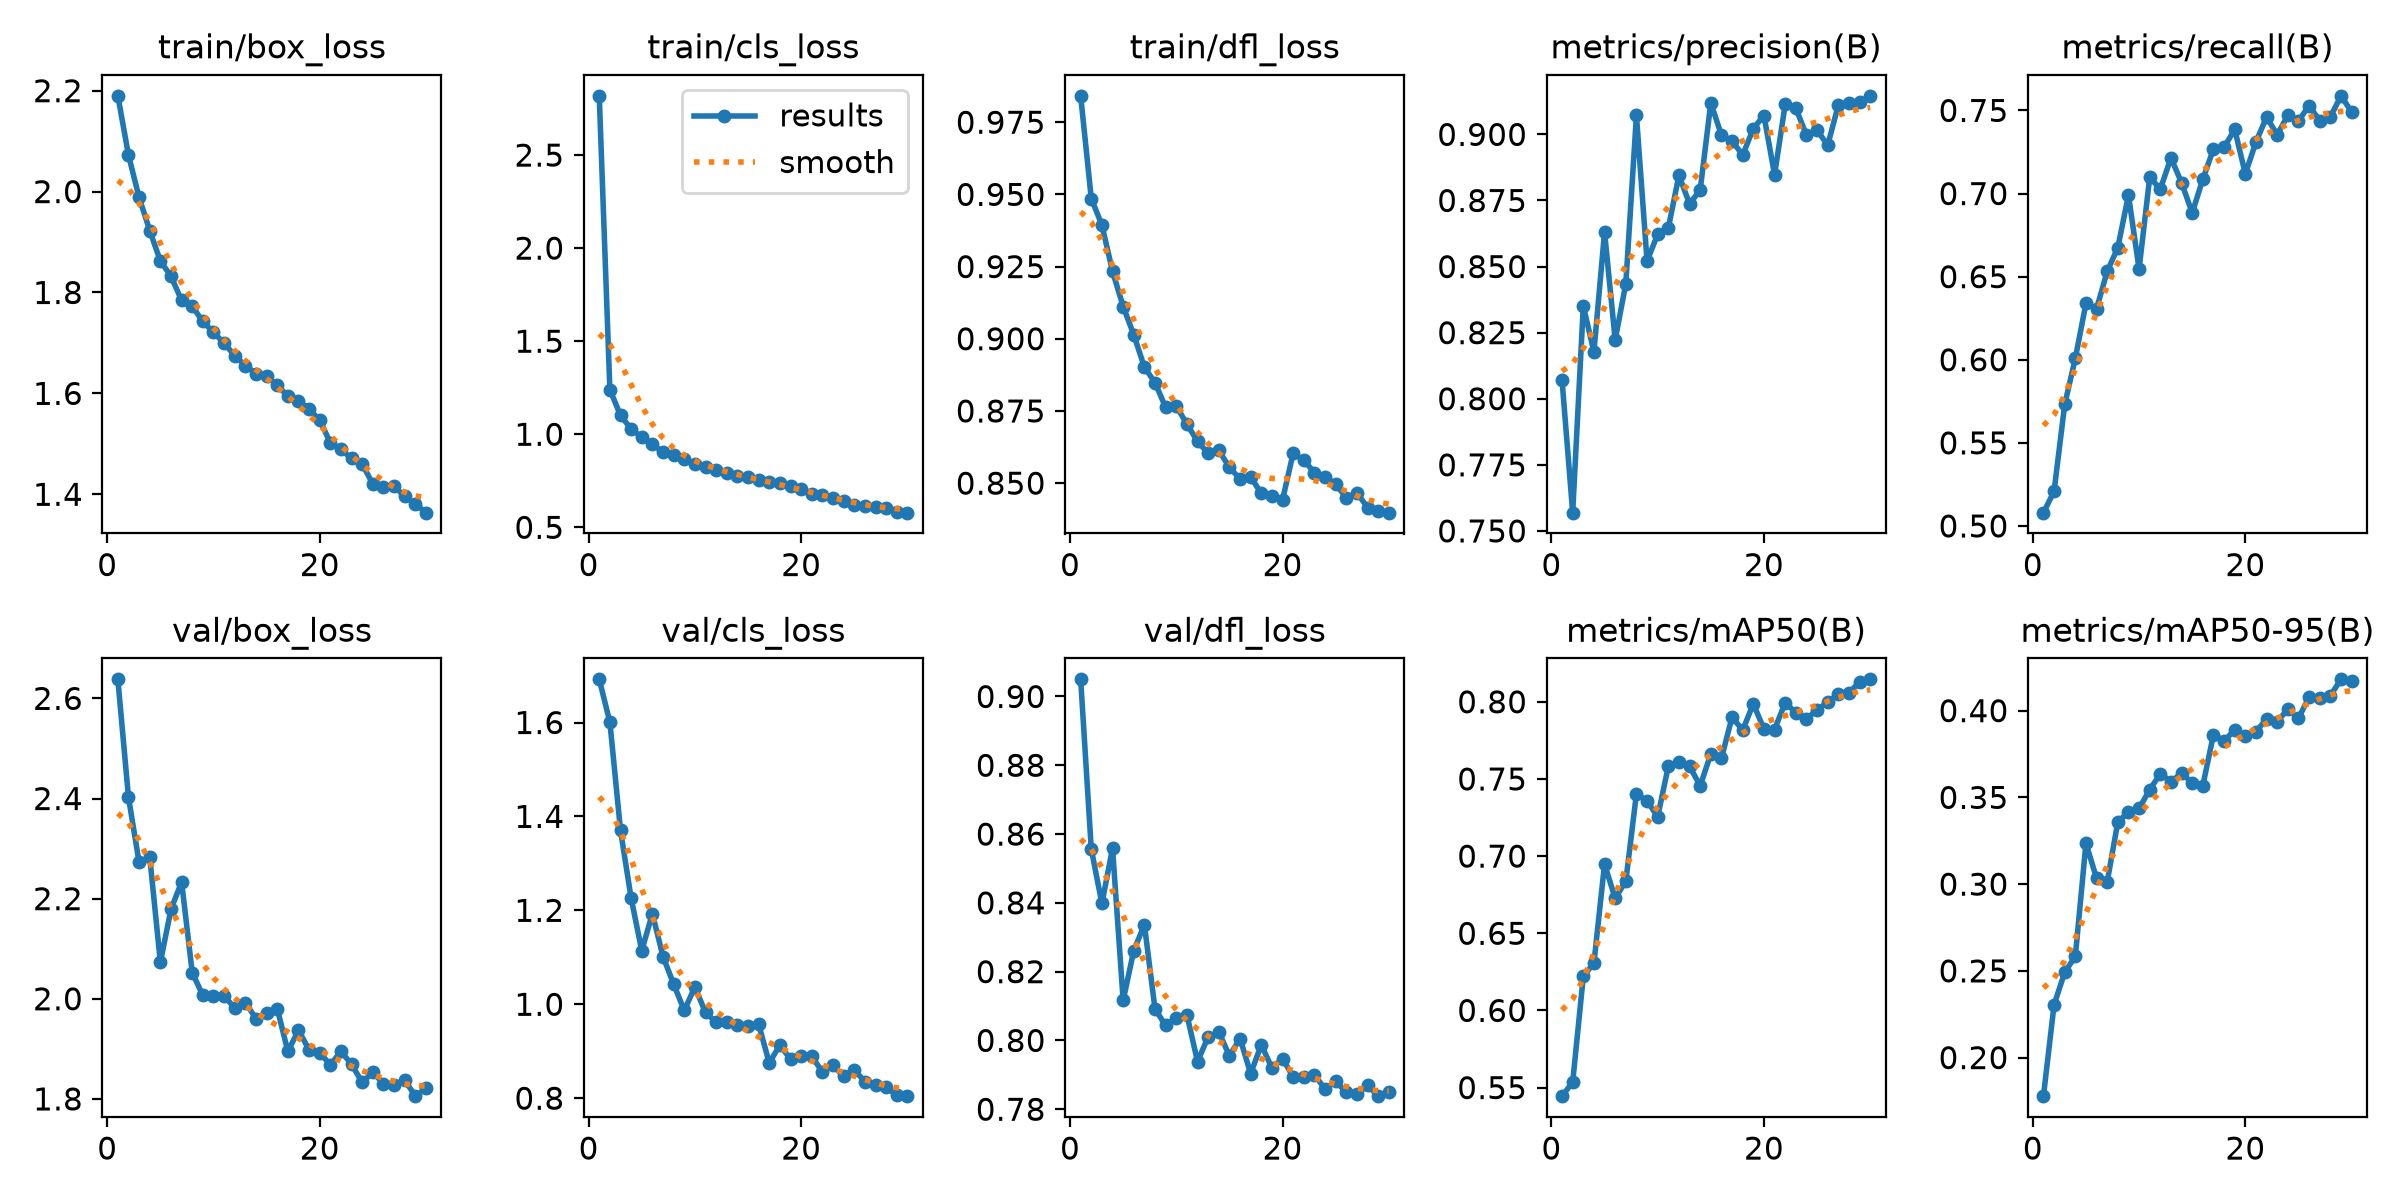
\includegraphics[width=0.47\textwidth]{images/pictures/training_curves_base.png}}
\hfill
\subfloat[YOLOv8n-P2-EMA]{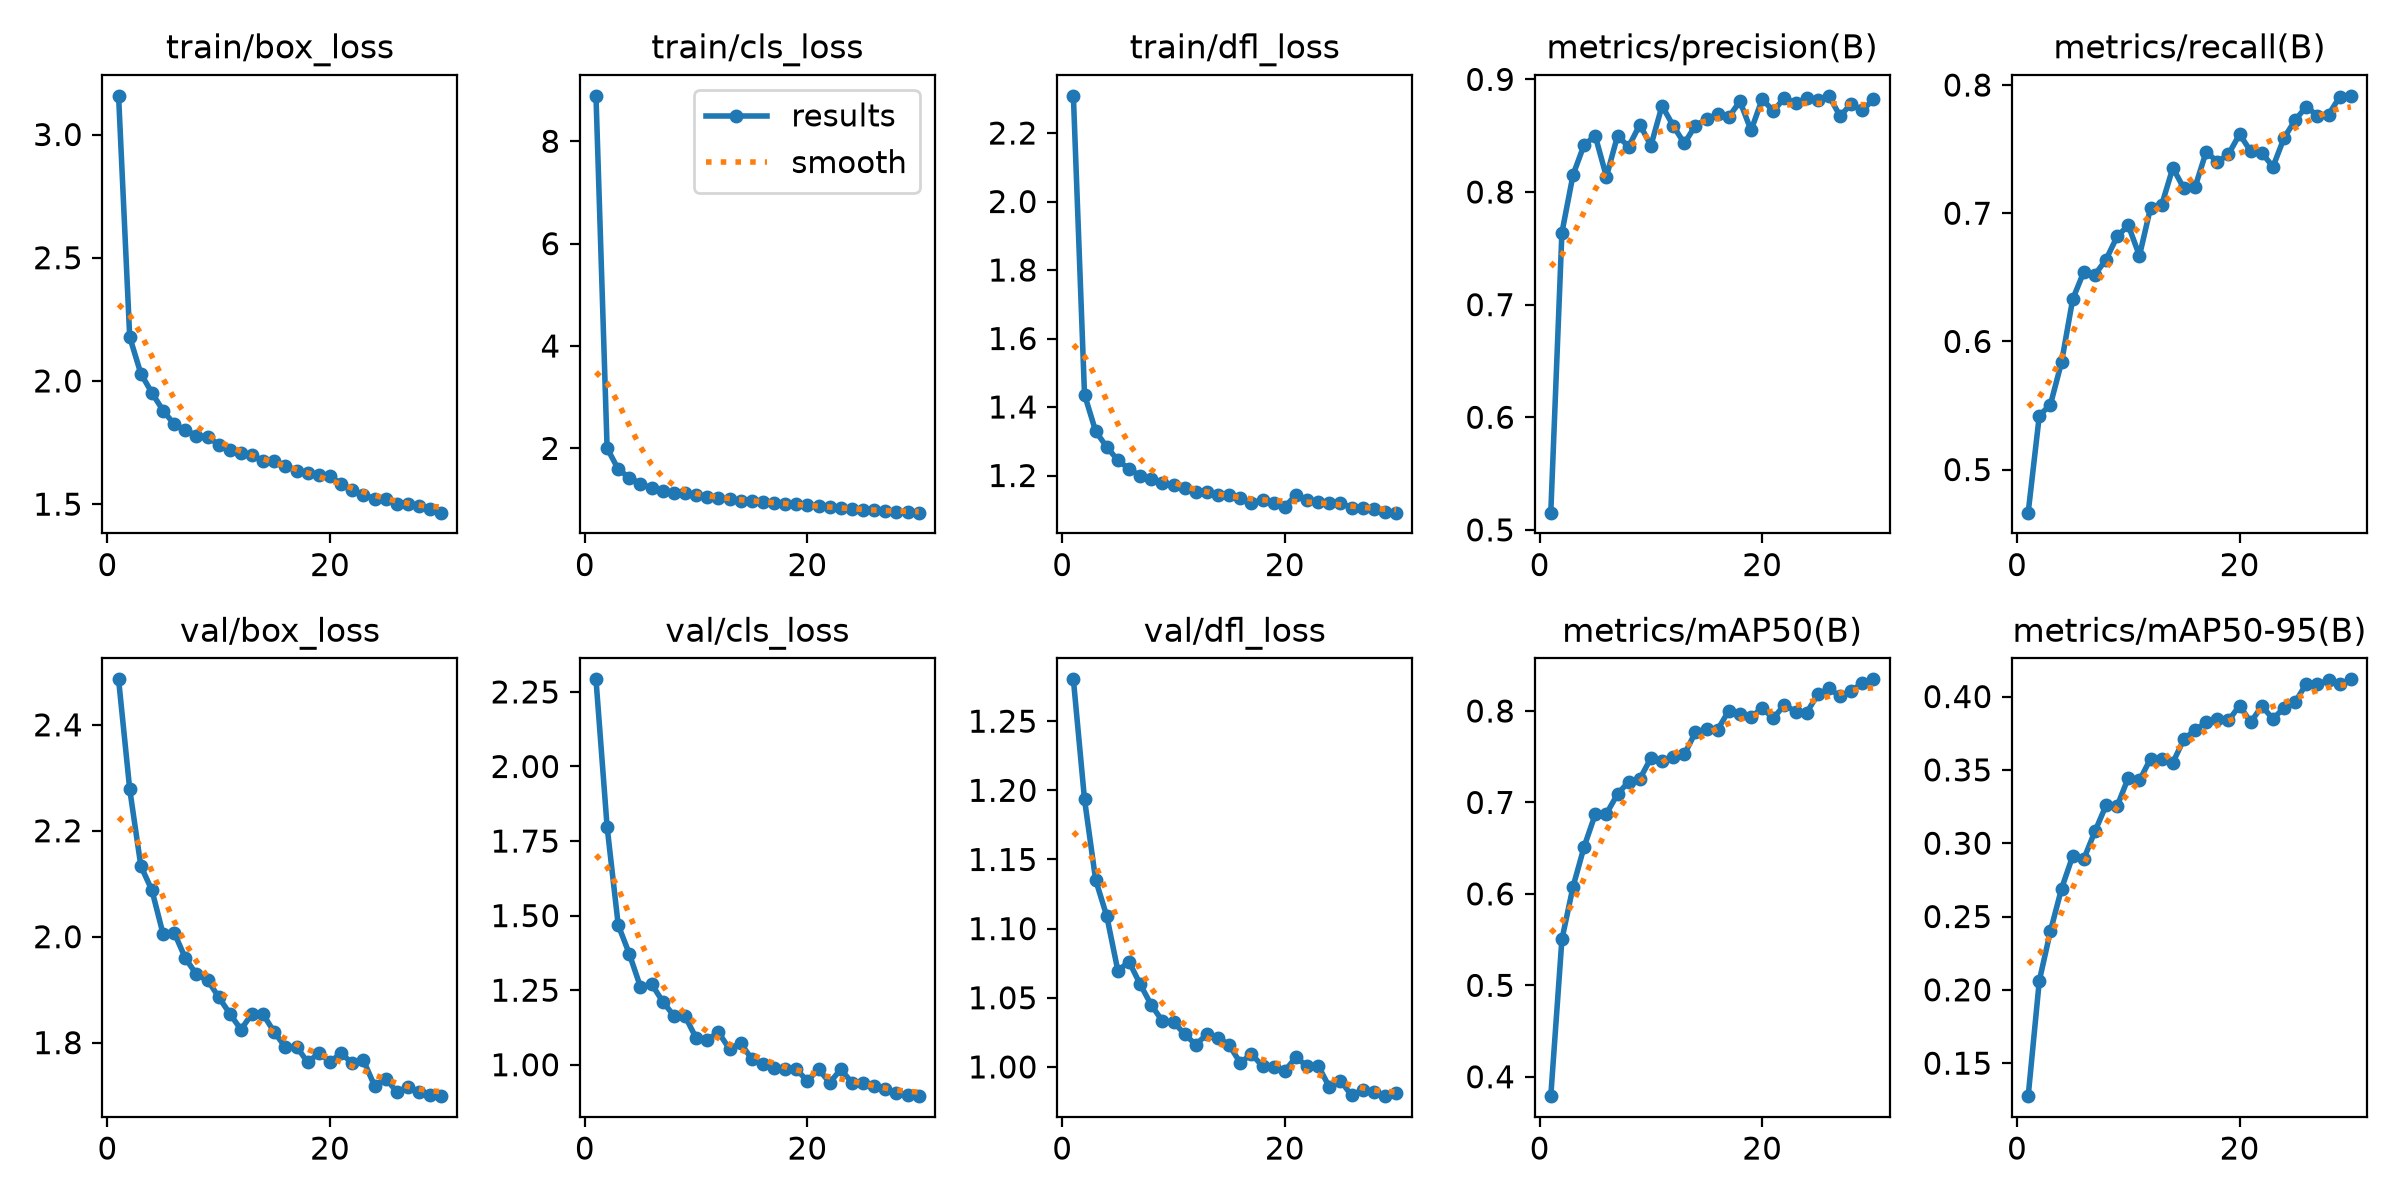
\includegraphics[width=0.47\textwidth]{images/pictures/training_curves_p2ema.png}}
\caption{训练损失与验证指标曲线}
\label{fig:training_curves}
\end{figure}

\section{消融实验}

\subsection{实验设置}

为验证 P2 与 EMA 各自的作用及组合效果，本文设计了四组对照实验：基线 YOLOv8n、+P2、+EMA、+P2+EMA。四组实验使用完全相同的数据划分、超参数与评测脚本，仅在网络结构上不同。评测在 Det-Fly 验证集上进行，输入 640，置信度阈值 0.001（mAP 计算需要低阈值以覆盖完整 P-R 曲线）。

\subsection{实验结果}

实验结果如表~\ref{tab:ablation} 所示。

\begin{table}[htbp]
\centering
\caption{检测模型消融实验（Det-Fly 验证集，imgsz=640）}
\label{tab:ablation}
\small
\begin{tabular}{lcccccccc}
\toprule
\textbf{模型} & \textbf{参数(M)} & \textbf{mAP50} & \textbf{mAP50-95} & \textbf{P} & \textbf{R} & \textbf{FPS} & \textbf{AP\_small} & \textbf{AP\_med} \\
\midrule
YOLOv8n（基线） & 3.01 & 81.3 & 41.8 & 91.2 & 75.9 & 123.0 & 6.1 & 77.0 \\
+P2 & 2.93 & 82.3 & 41.3 & 88.9 & 77.6 & 90.3 & 8.3 & 76.2 \\
+EMA & 3.02 & 76.2 & 36.3 & 85.5 & 72.2 & 101.0 & 4.1 & 75.0 \\
+P2+EMA（本文） & 2.94 & \textbf{83.5} & 41.2 & 88.2 & \textbf{79.2} & 98.4 & \textbf{9.8} & \textbf{78.0} \\
\bottomrule
\end{tabular}
\end{table}

表中所有指标单位为百分数，FPS 为帧每秒。AP\_small 为 COCO 面积口径、IoU=0.5、101 点插值。

\subsection{结果分析}

\textbf{（1）P2 单独作用}。mAP50 从 81.3\% 提升至 82.3\%，Recall 从 75.9\% 提升至 77.6\%，AP\_small 从 6.1\% 提升至 8.3\%，相对提升 36.1\%。这说明高分辨率检测层确实增强了小目标召回。与此同时，Precision 从 91.2\% 降至 88.9\%，mAP50-95 略降 0.5 个百分点，原因是 P2 层引入了更多弱响应，部分背景被误检。FPS 从 123 降至 90，符合计算量分析。

\textbf{（2）EMA 单独作用}。结果看似异常：mAP50 降至 76.2\%，AP\_small 仅 4.1\%，甚至低于基线。这一现象不能简单解释为"EMA 无效"。本文的分析是：EMA 的注意力重加权在缺乏高分辨率特征时，会把权重集中在 P3/P4 上已经模糊的目标区域，而这些区域的边界信息不足以支撑精确定位；同时，注意力对背景的抑制过于激进，导致部分低置信度的真实目标被"压"到阈值以下。换言之，EMA 需要一张"看得清"的特征图才能发挥"认得准"的作用。

\textbf{（3）P2+EMA 的互补性}。两者联合后，mAP50 达到 83.5\%，Recall 79.2\%，AP\_small 9.8\%，均为四组最优。AP\_small 相对基线提升 60.7\%，相对 +P2 提升 18.1\%。这一结果支持了"P2 提供分辨率、EMA 提供判别力"的解释：P2 让目标在特征图上占据足够多的网格，EMA 在这些网格上进一步区分目标与背景，二者形成正向互补。

\textbf{（4）参数效率}。本文模型的参数量为 2.94\,M，低于基线的 3.01\,M，却取得了最优的 mAP50 与 AP\_small。这说明性能提升并非来自模型容量扩张，而是来自特征利用效率的改善。对于部署在边缘设备上的反无人机系统，这一特性尤为重要。

\textbf{（5）速度}。本文模型 FPS 为 98.4，约为基线的 80\%，但仍为 30\,fps 视频帧率的 3 倍以上。考虑到系统还需要进行卡尔曼滤波、界面绘制与网络通信，保留 2--3 倍余量是必要的。

\subsection{混淆矩阵与 P-R 曲线}

图~\ref{fig:confusion} 给出了基线模型与本文模型的混淆矩阵。两者在"背景误检"上的差异不大，本文模型的漏检（真值为正、预测为背景）明显减少，这与 Recall 的提升一致。

\begin{figure}[htbp]
\centering
\subfloat[基线 YOLOv8n]{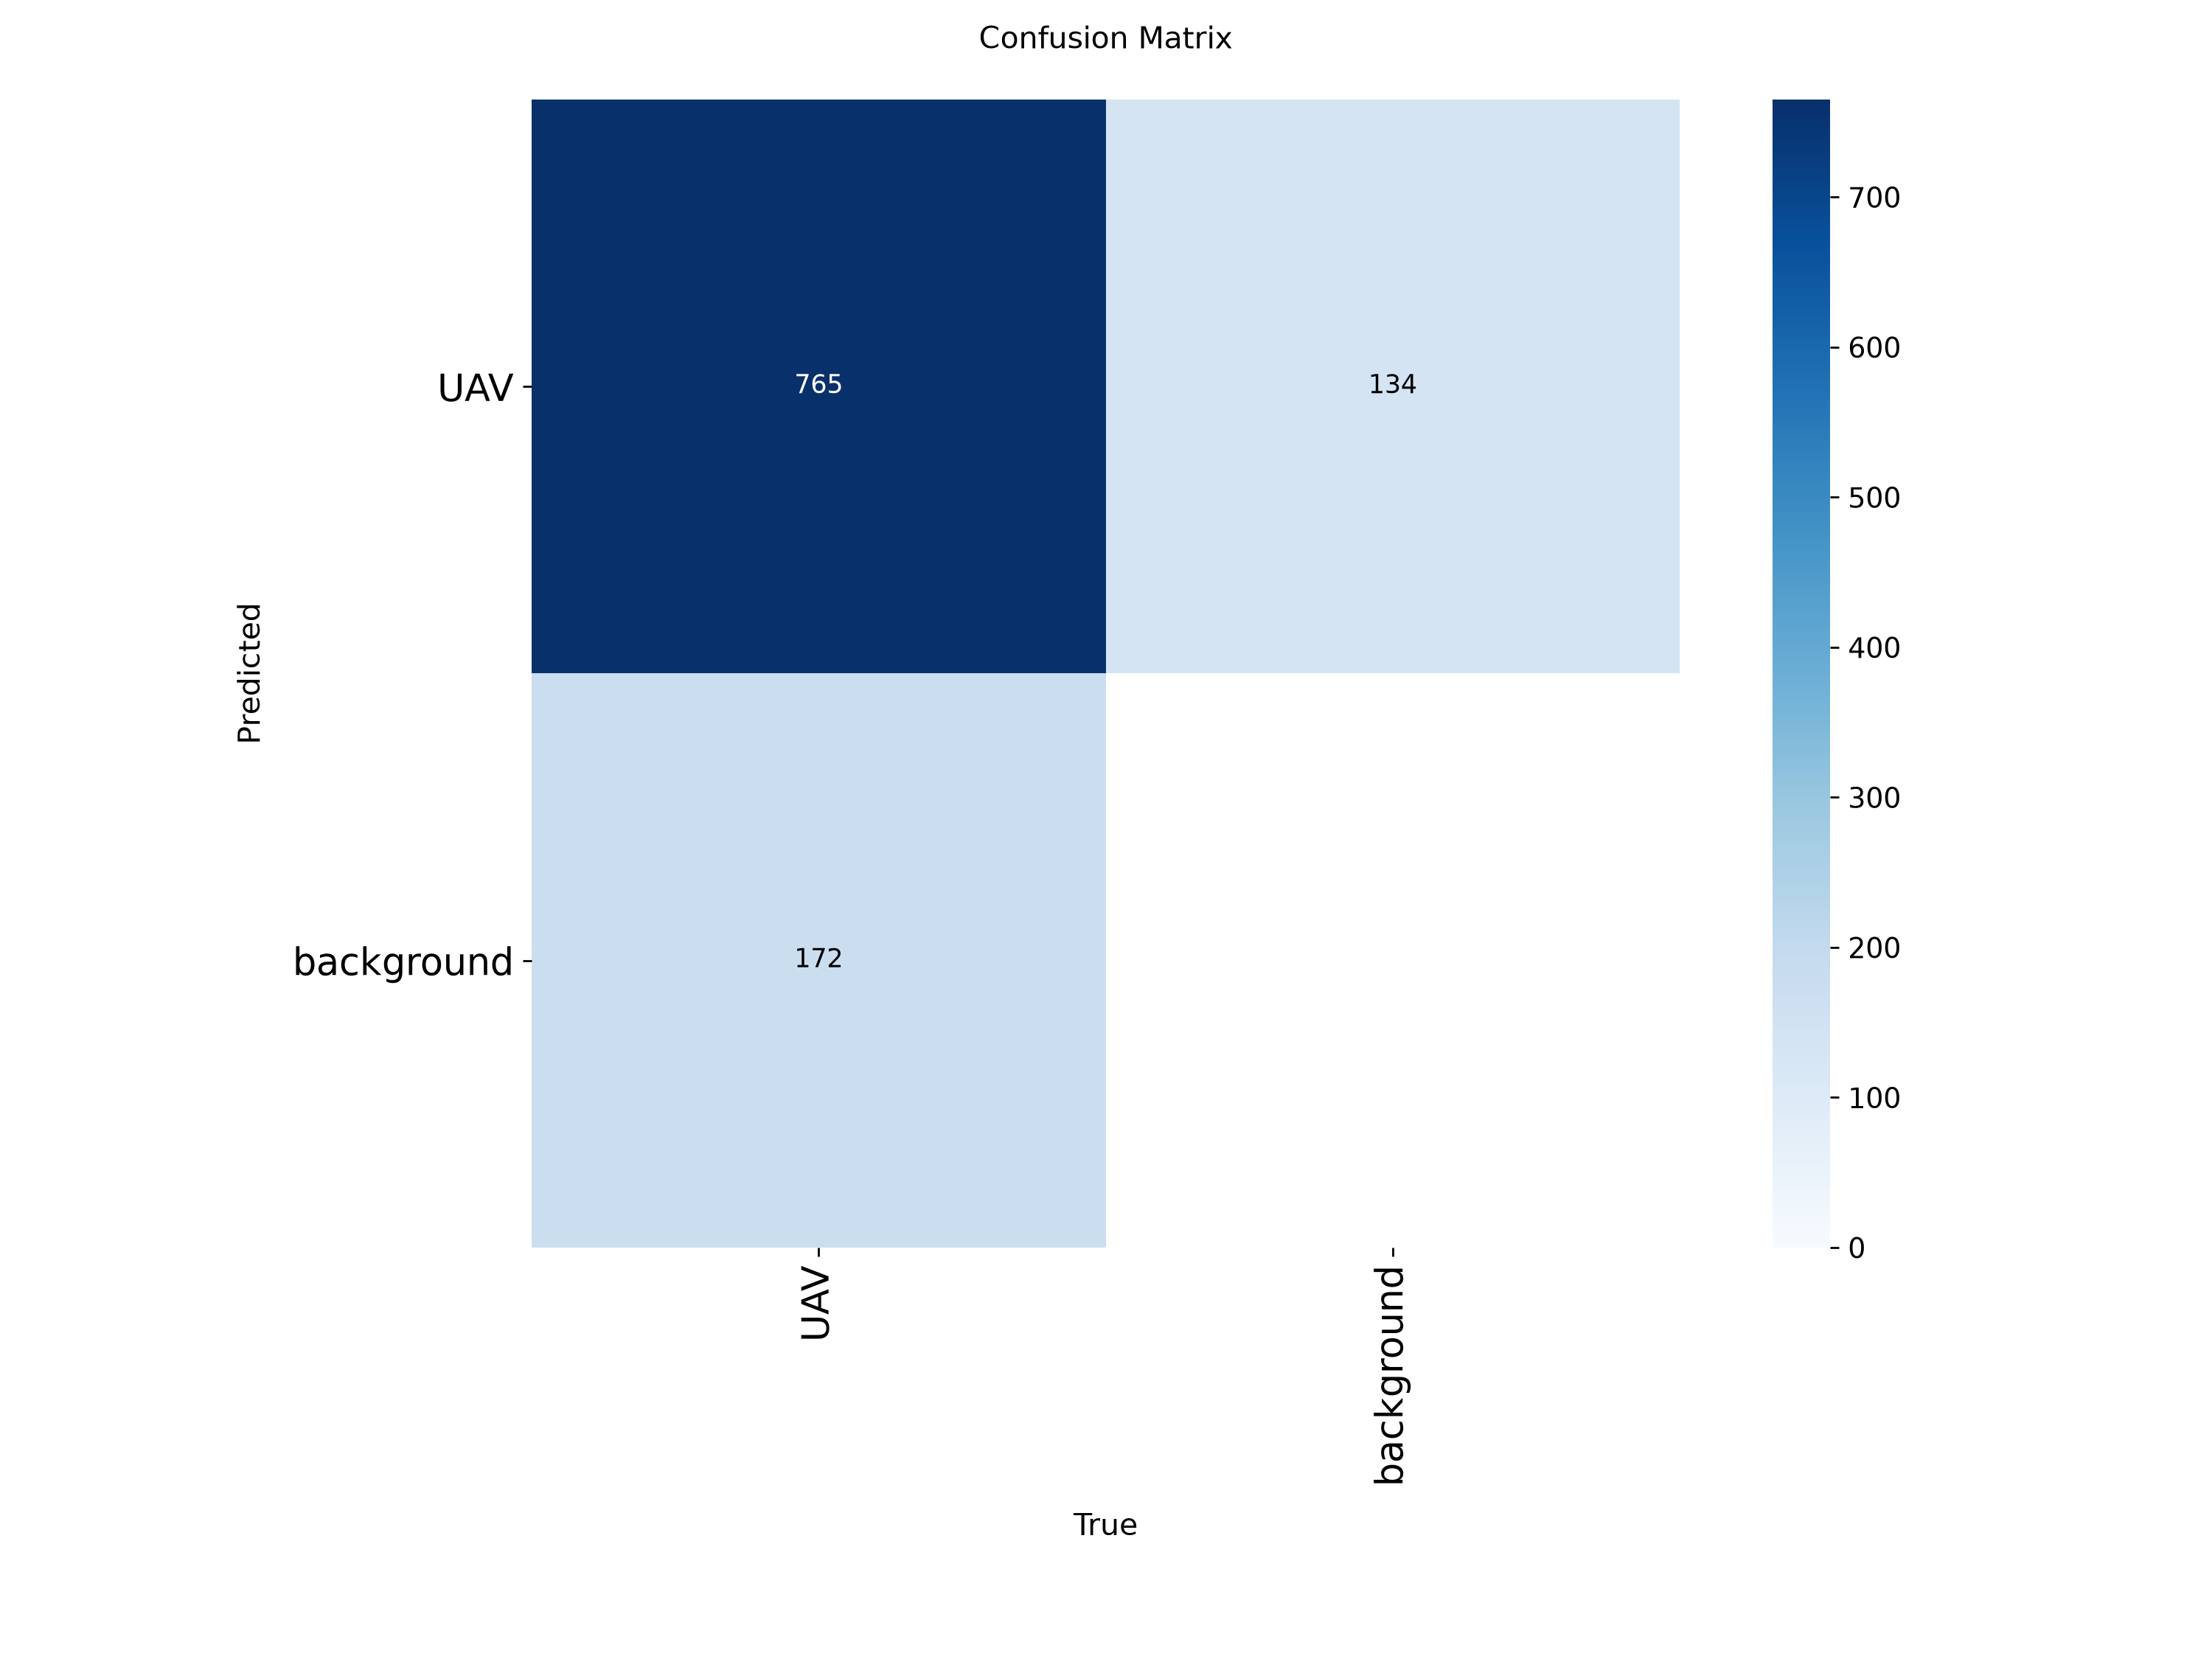
\includegraphics[width=0.45\textwidth]{images/pictures/confusion_matrix_base.png}}
\hfill
\subfloat[YOLOv8n-P2-EMA]{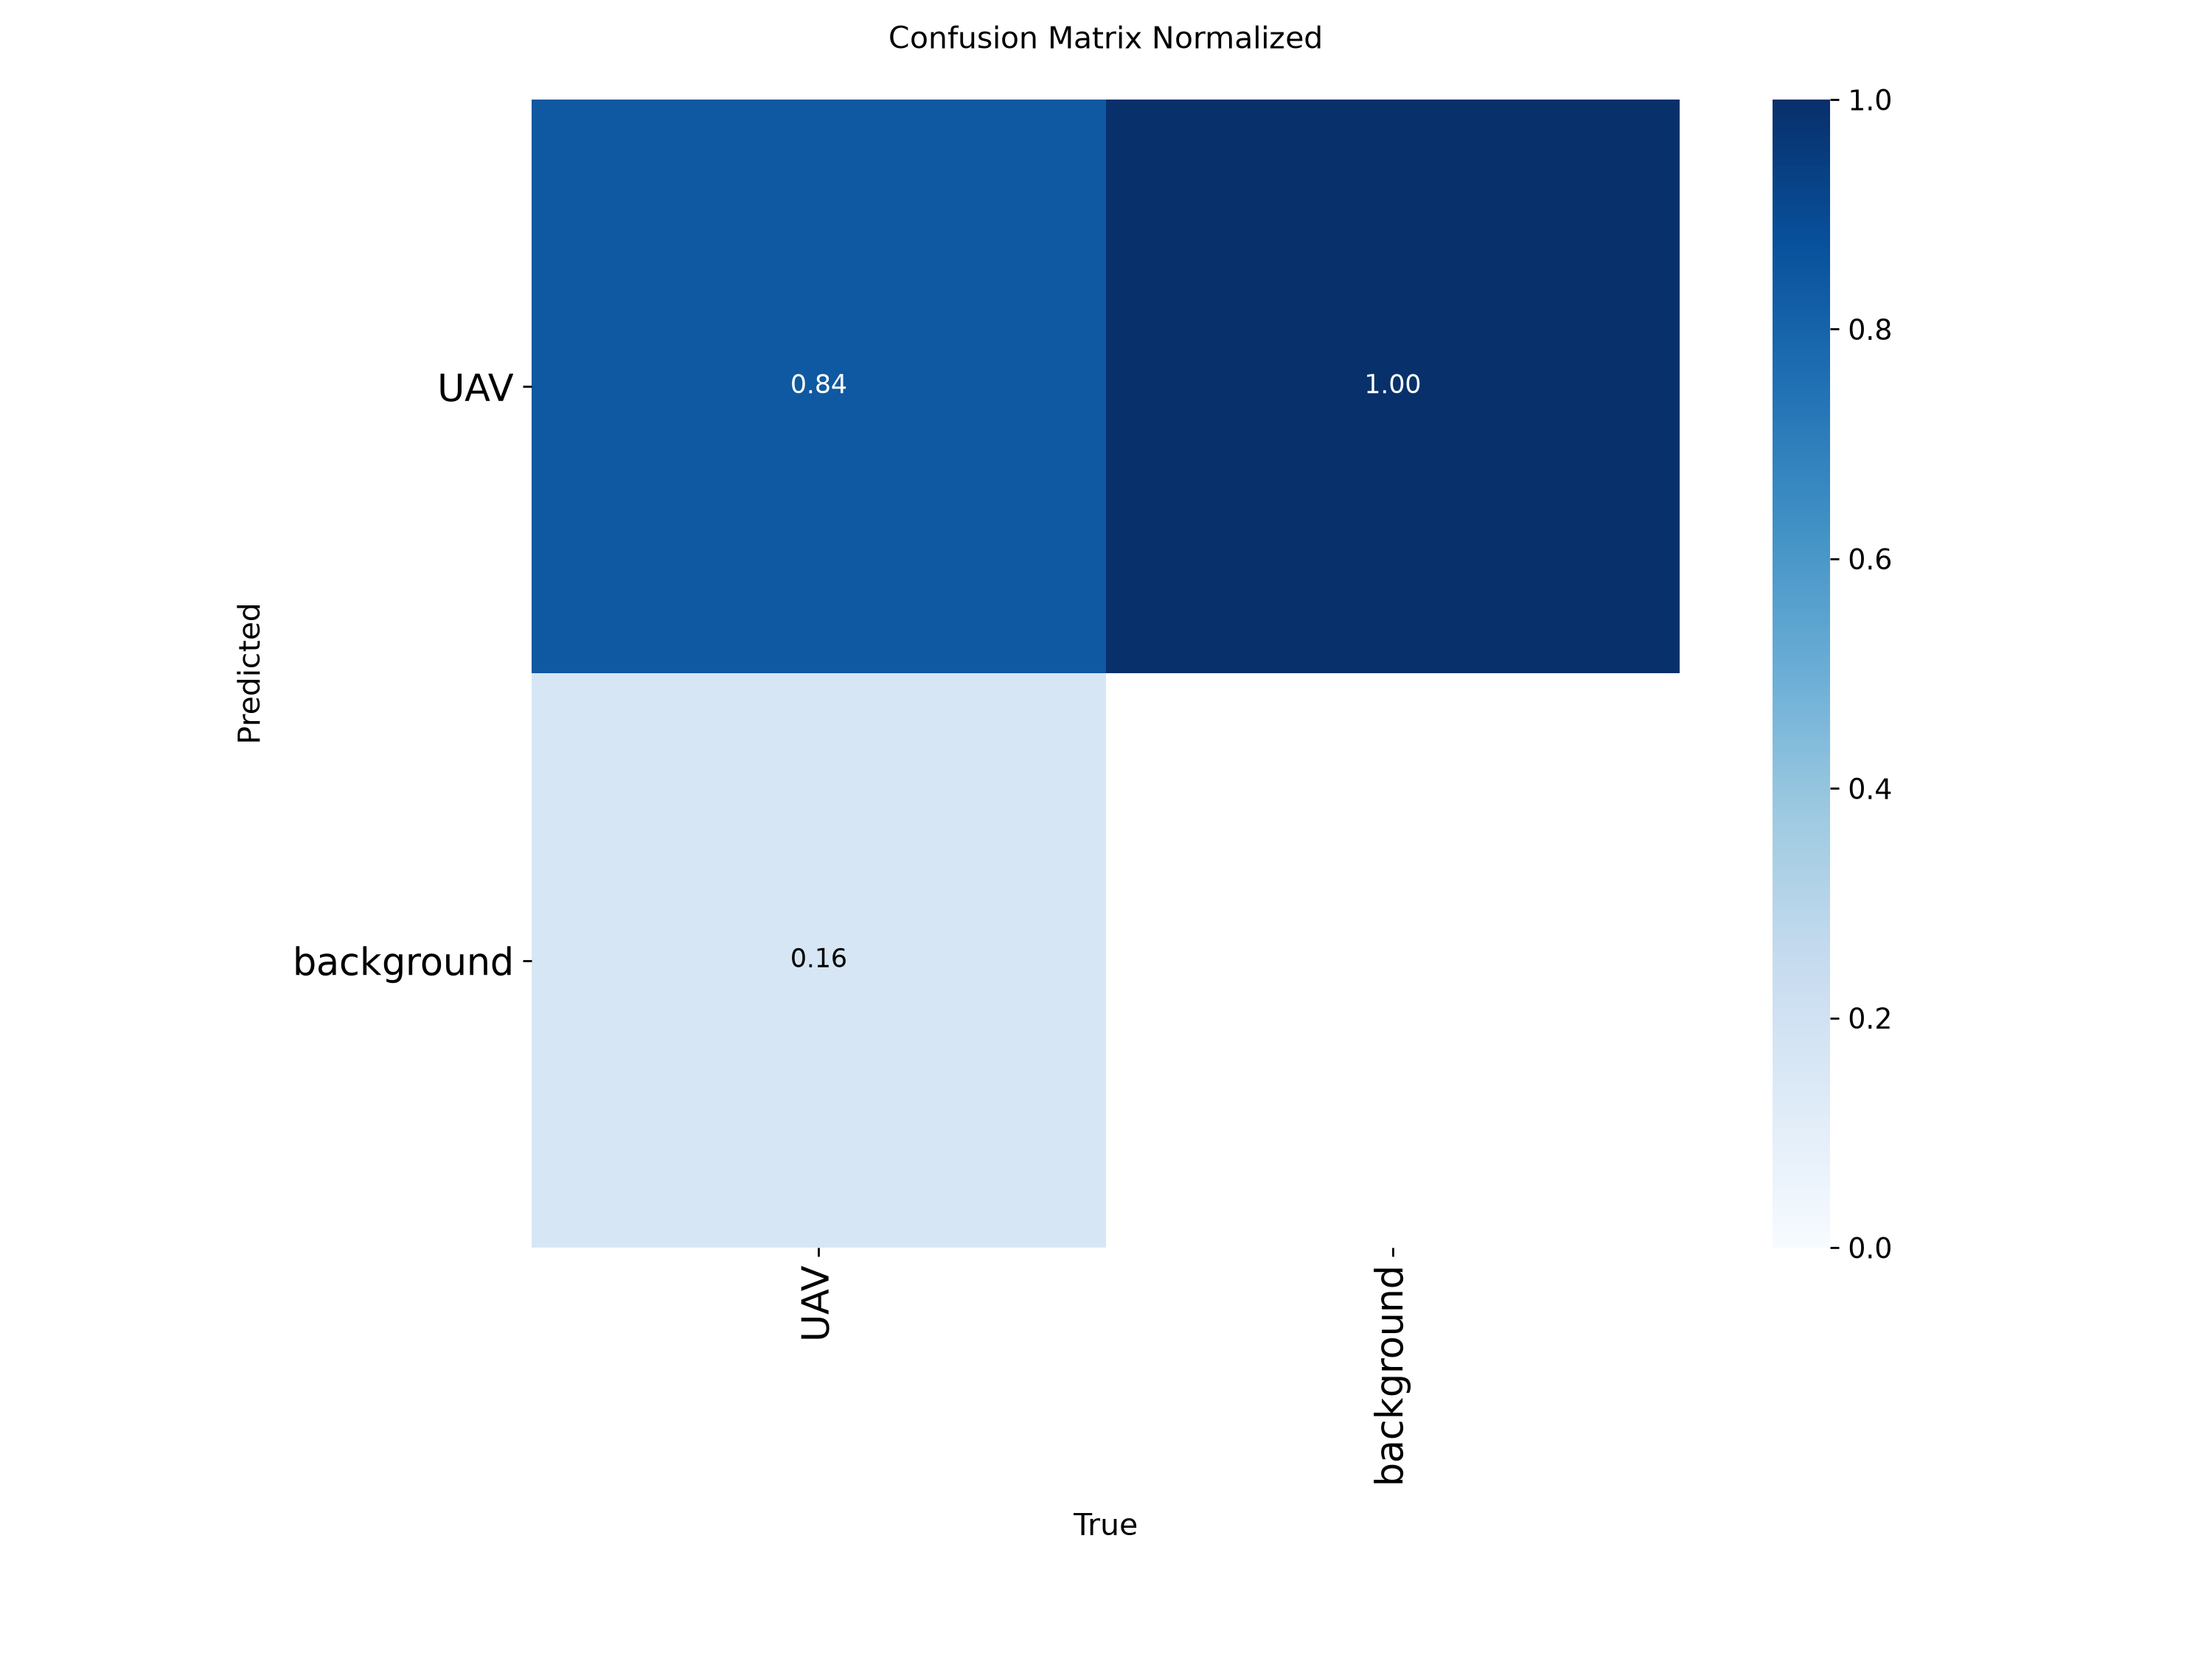
\includegraphics[width=0.45\textwidth]{images/pictures/confusion_matrix_p2ema.png}}
\caption{验证集混淆矩阵}
\label{fig:confusion}
\end{figure}

图~\ref{fig:pr_f1} 给出了本文模型的 P-R 曲线与 F1 曲线。P-R 曲线在高召回区间的"尾部"比基线更饱满，说明模型在低置信度区域仍能保持一定的精度，这对后续状态机的低门限初筛是有利的。

\begin{figure}[htbp]
\centering
\subfloat[P-R 曲线]{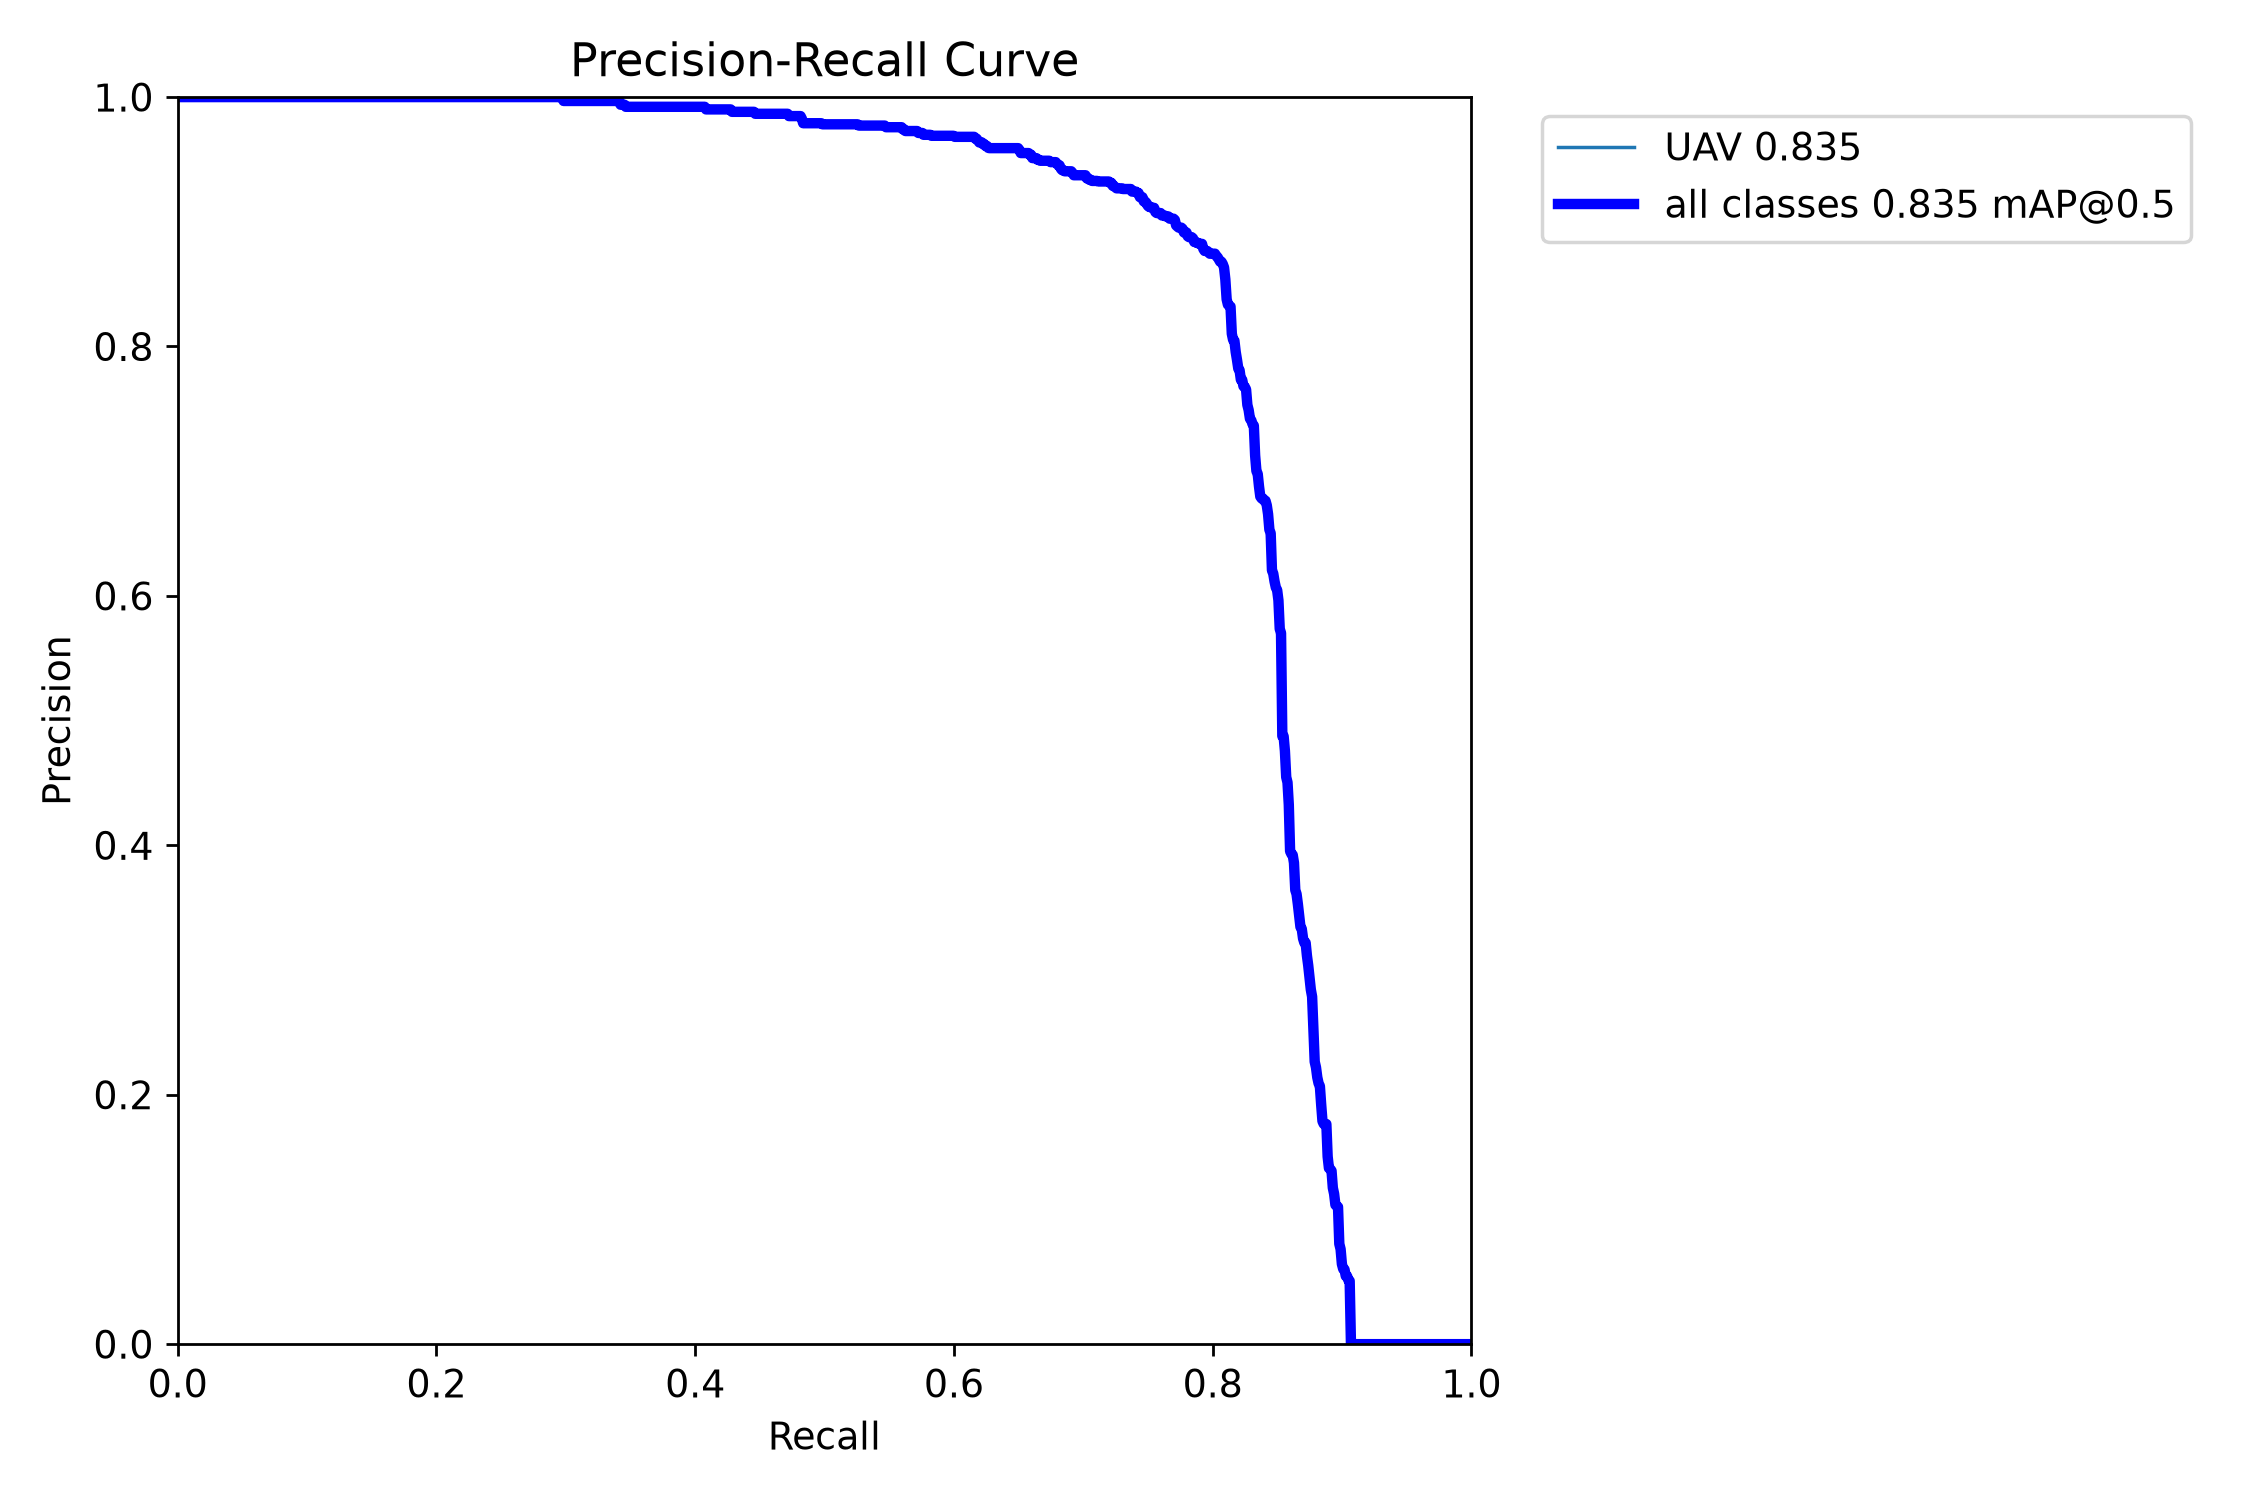
\includegraphics[width=0.47\textwidth]{images/pictures/pr_curve_p2ema.png}}
\hfill
\subfloat[F1-置信度曲线]{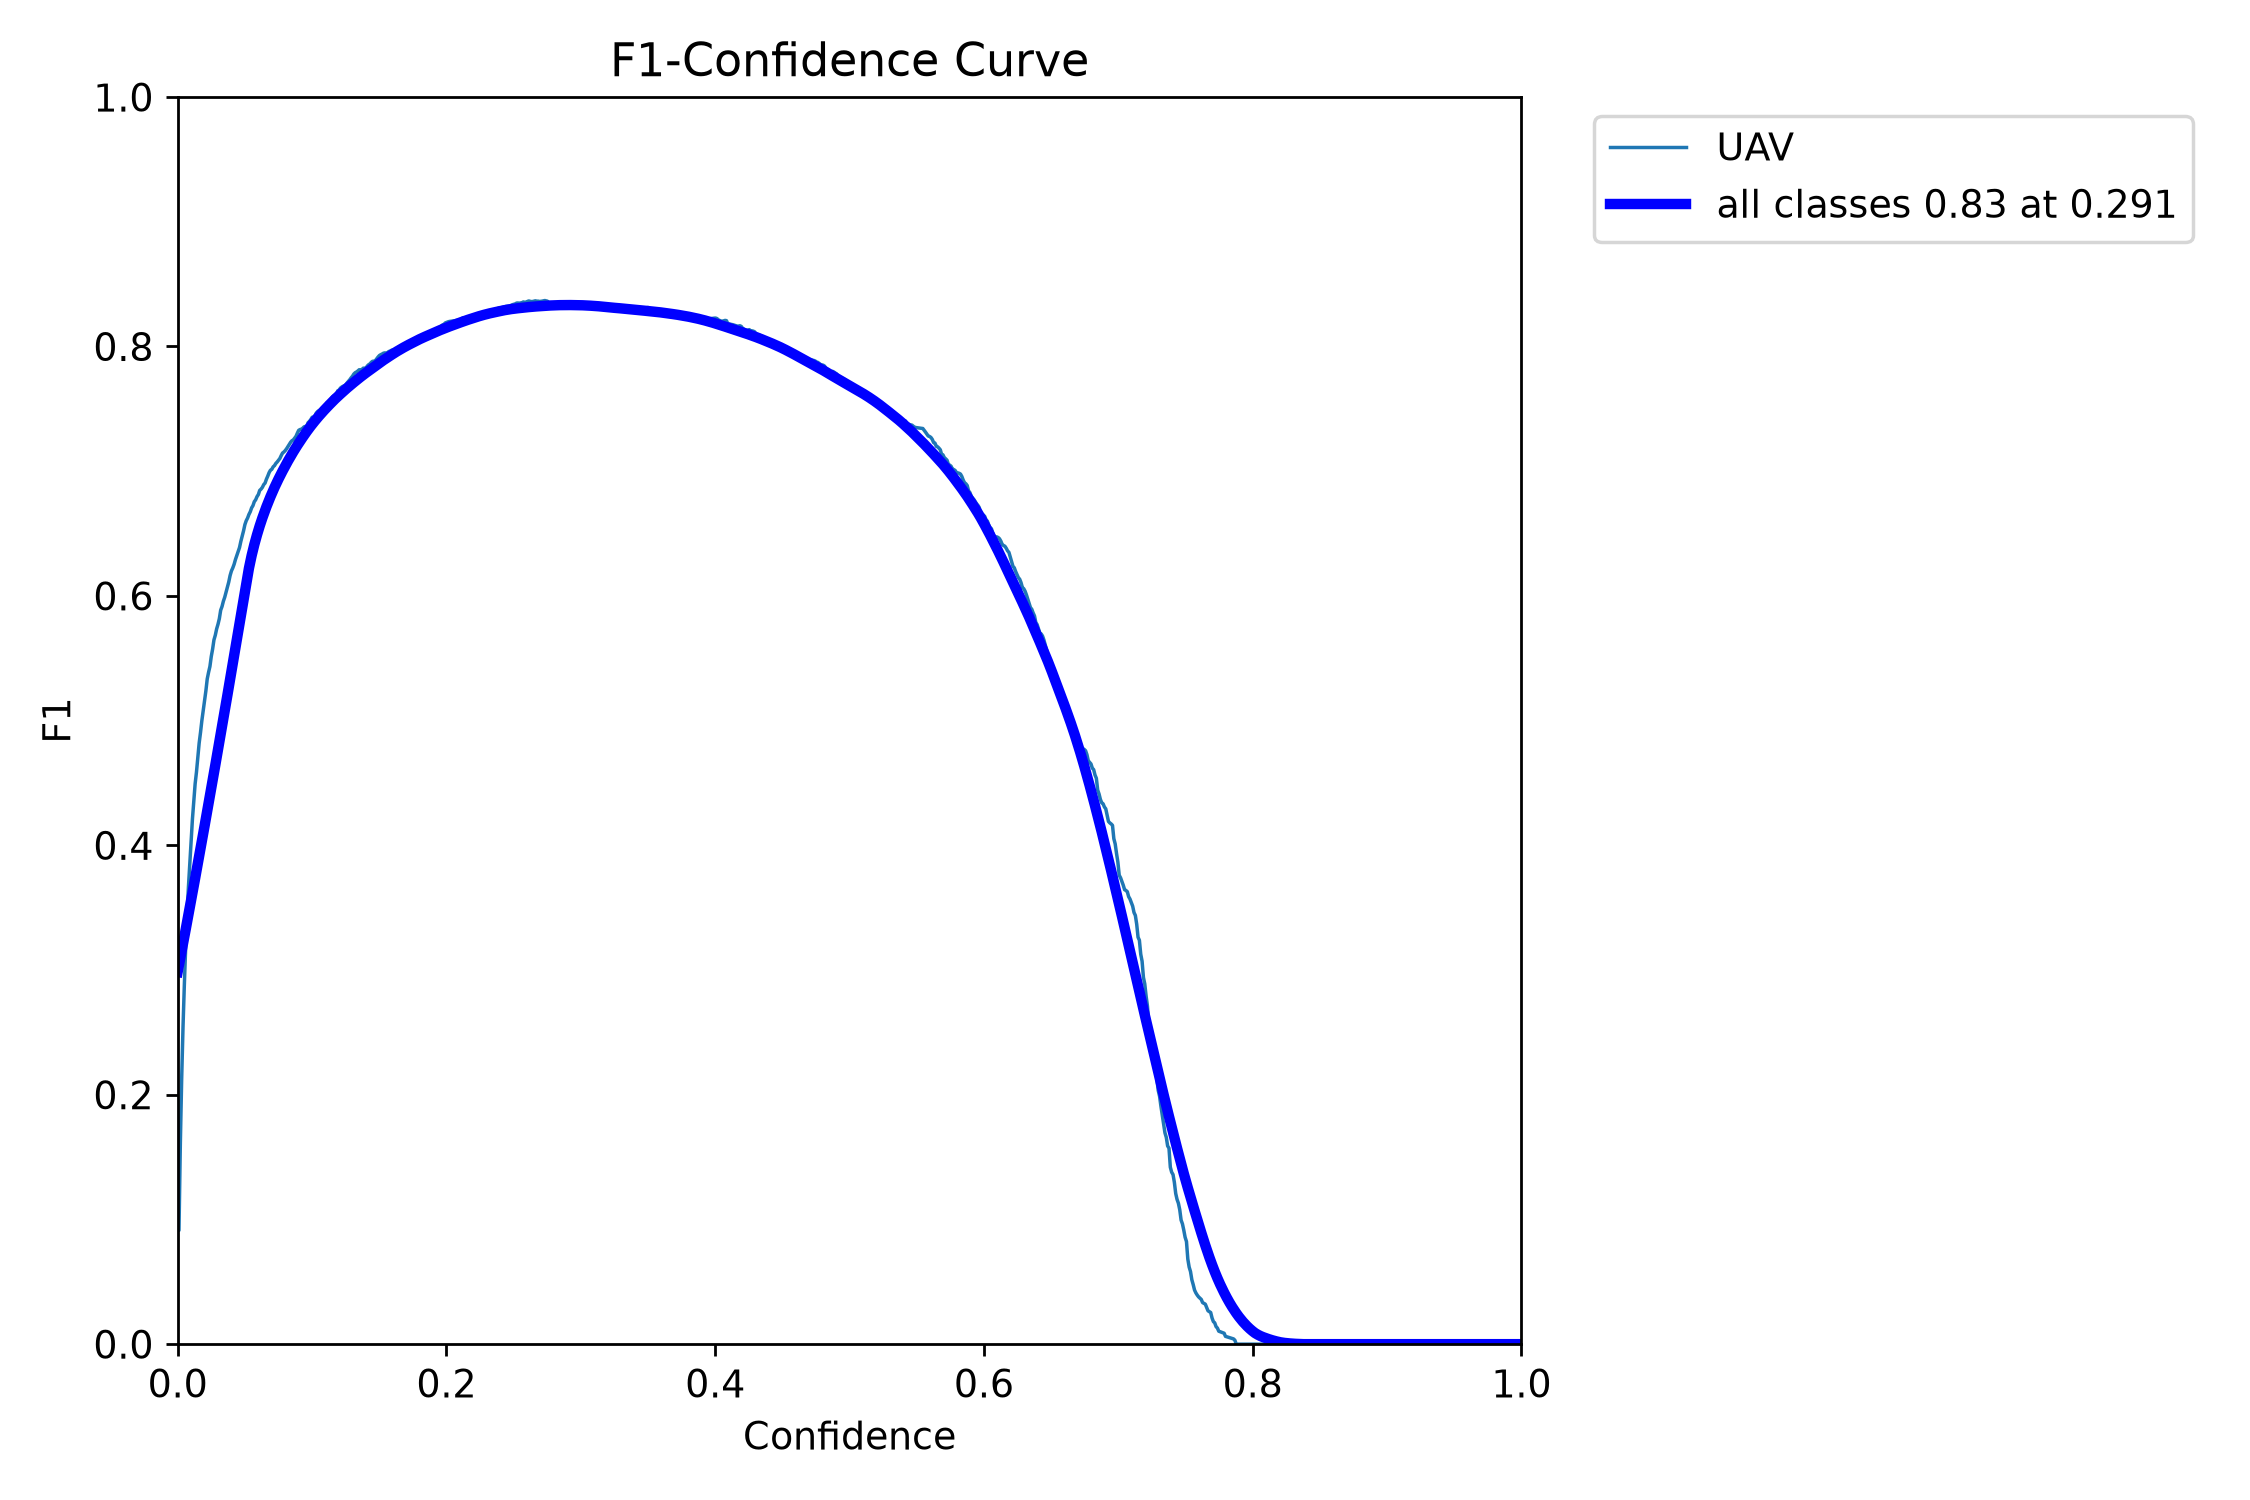
\includegraphics[width=0.47\textwidth]{images/pictures/f1_curve_p2ema.png}}
\caption{YOLOv8n-P2-EMA 的 P-R 与 F1 曲线}
\label{fig:pr_f1}
\end{figure}

\subsection{检测效果可视化}

图~\ref{fig:val_predictions} 展示了验证集的批量预测结果。绿色框为真值，红色框为预测。可以看到，本文模型在目标较小、背景复杂的场景中仍能给出稳定的框，框的边界与真值吻合较好。

\begin{figure}[htbp]
\centering
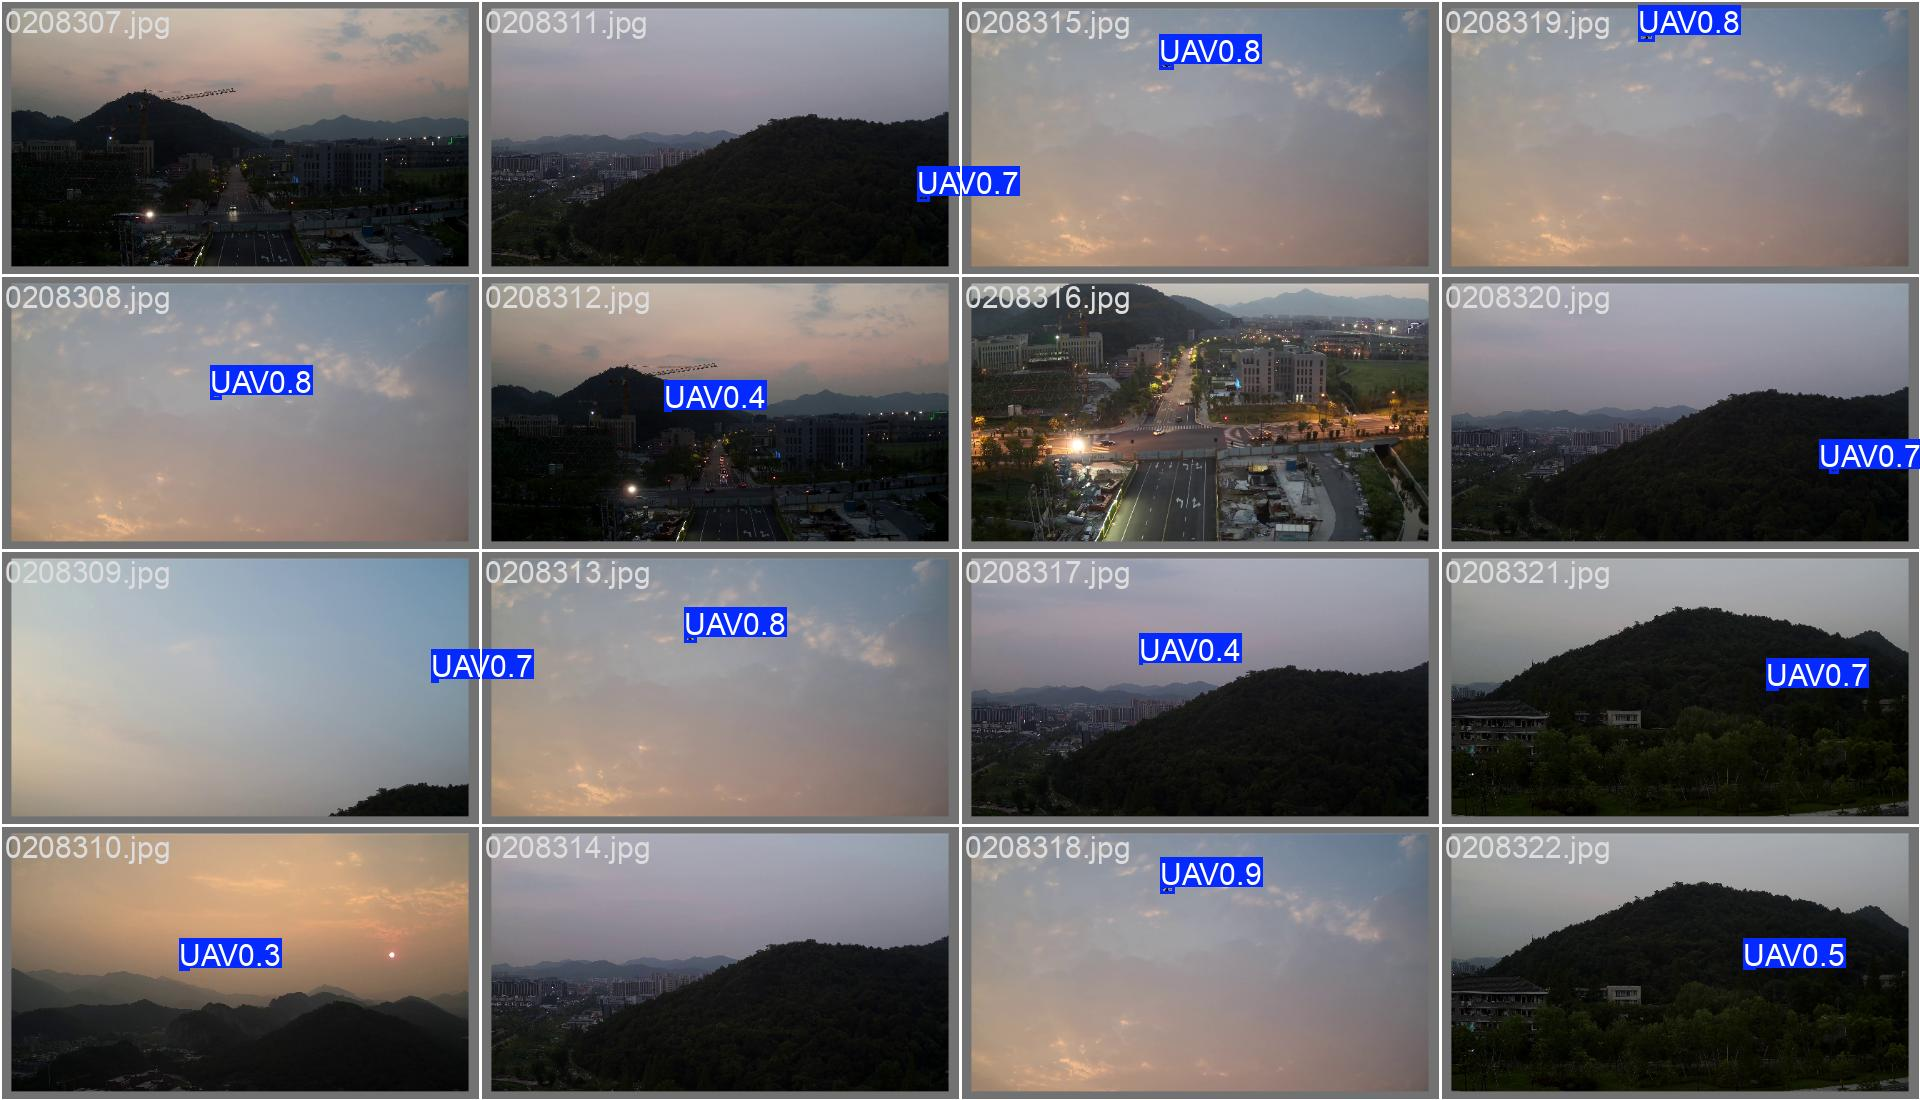
\includegraphics[width=0.92\textwidth]{images/pictures/val_predictions.jpg}
\caption{验证集批量预测结果（绿框为真值，红框为预测）}
\label{fig:val_predictions}
\end{figure}

图~\ref{fig:compare} 给出了四组典型帧的对比，按"基线置信度与本文置信度差异"排序选取，用于直观展示改进在困难样本上的效果。蓝色虚线框为真值，实线框为预测。

\begin{figure}[htbp]
\centering
\subfloat[样本一]{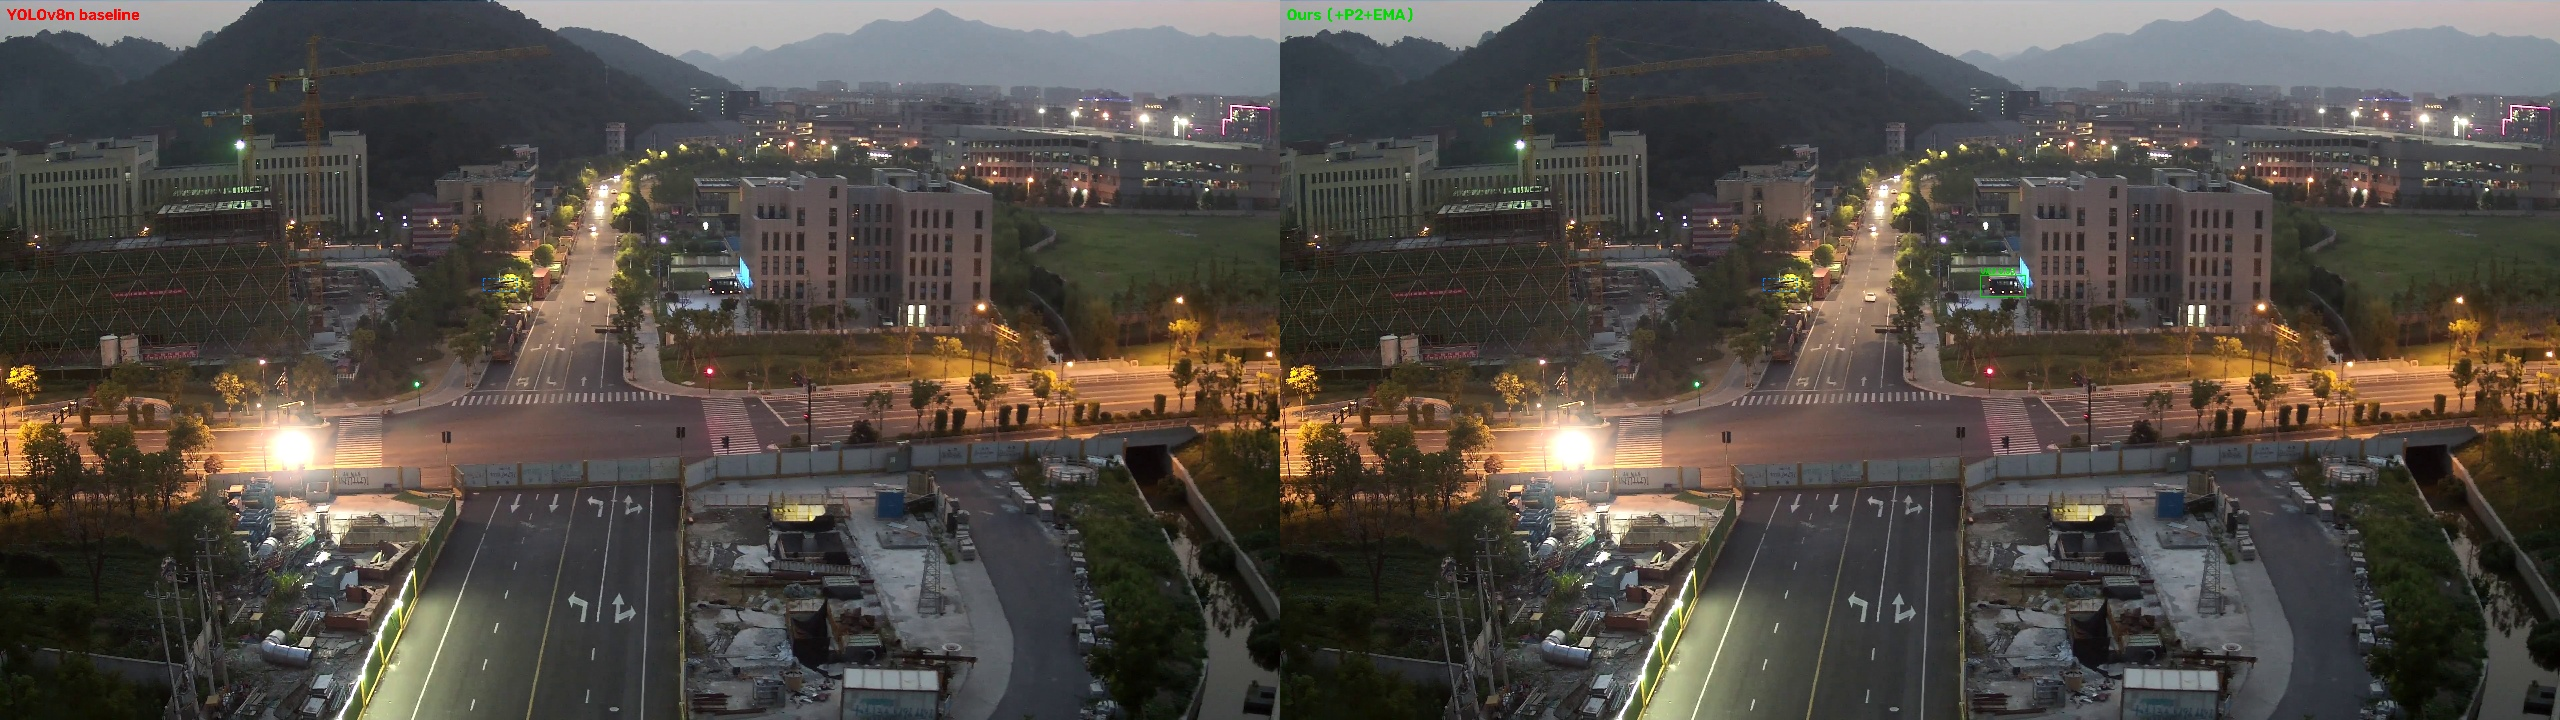
\includegraphics[width=0.48\textwidth]{images/pictures/compare_01.jpg}}
\hfill
\subfloat[样本二]{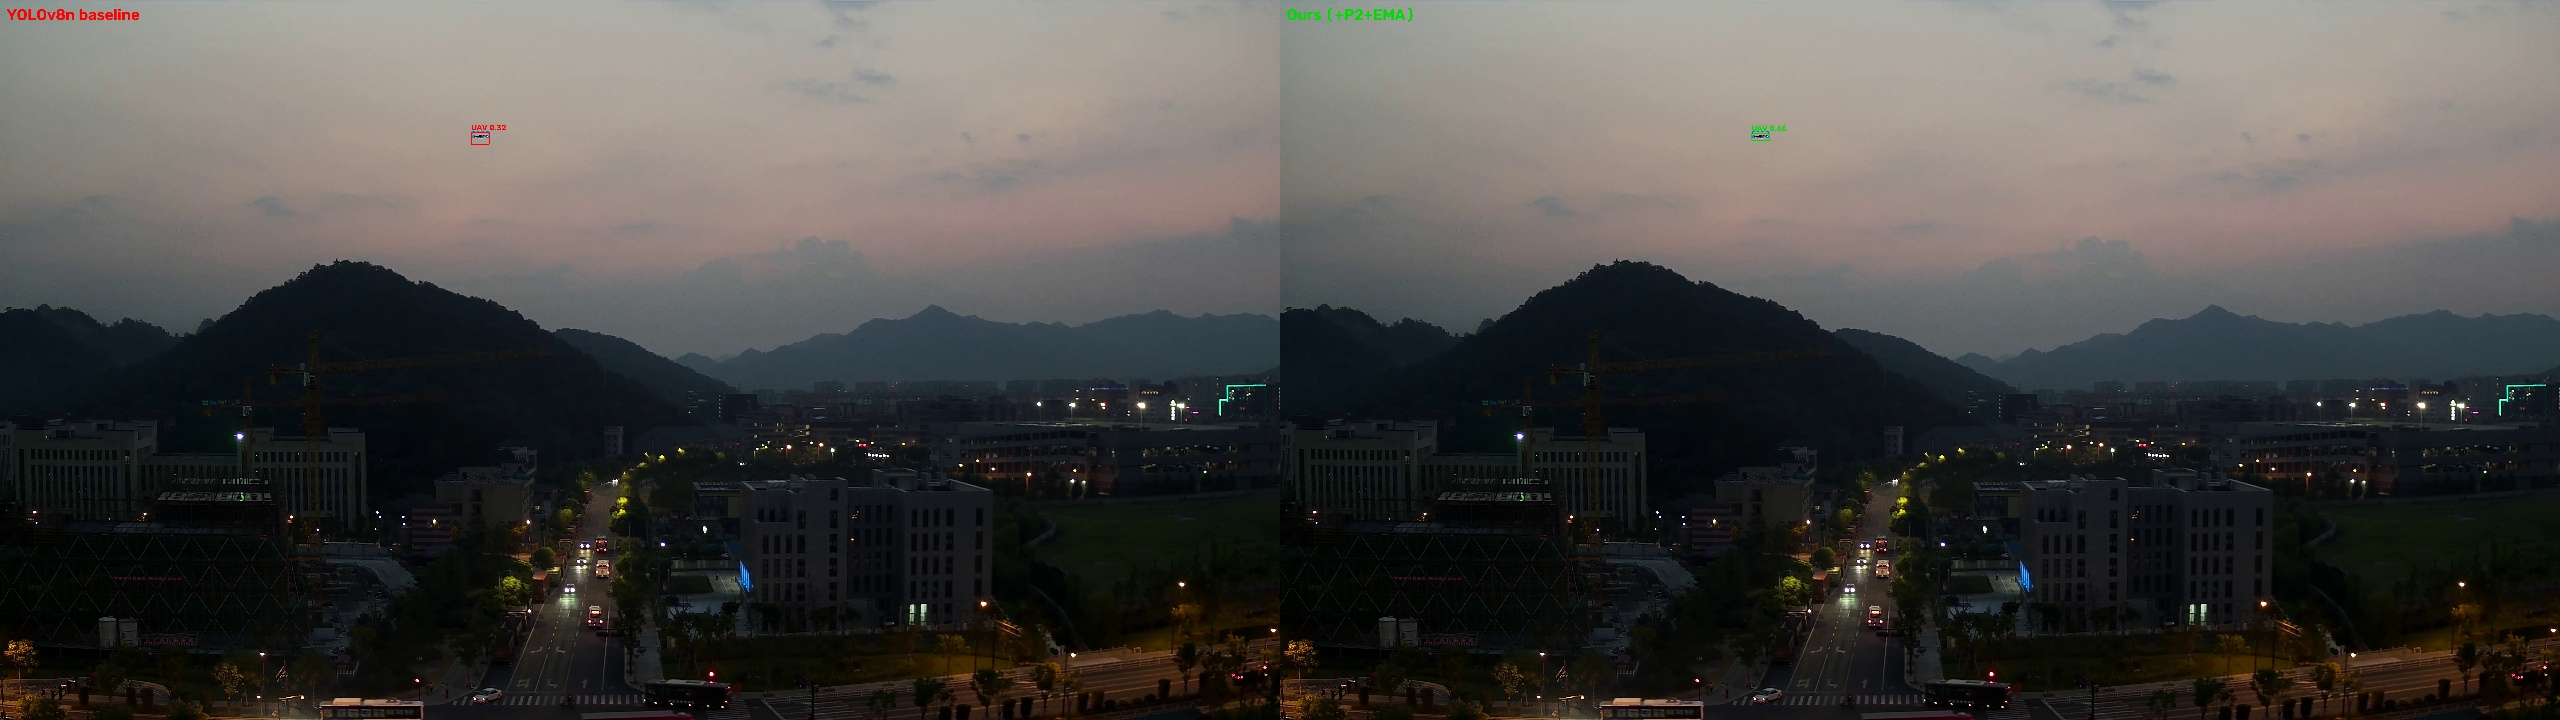
\includegraphics[width=0.48\textwidth]{images/pictures/compare_02.jpg}}\\
\subfloat[样本三]{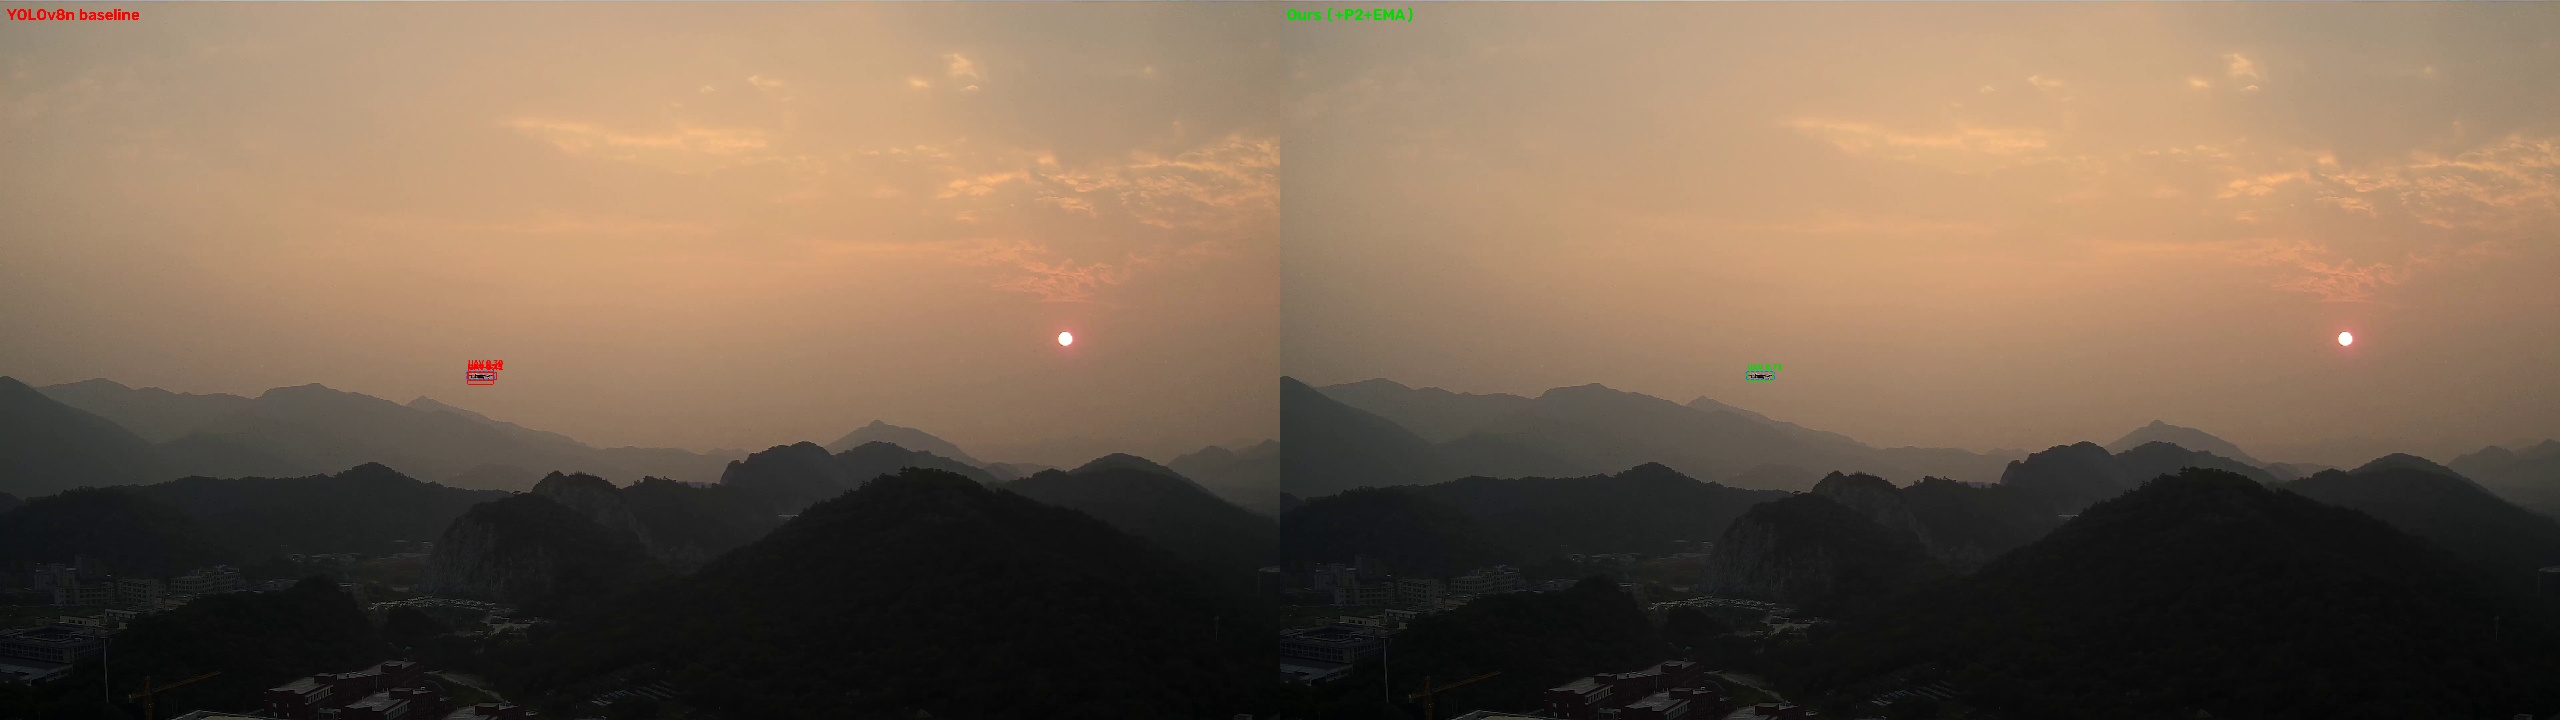
\includegraphics[width=0.48\textwidth]{images/pictures/compare_03.jpg}}
\hfill
\subfloat[样本四]{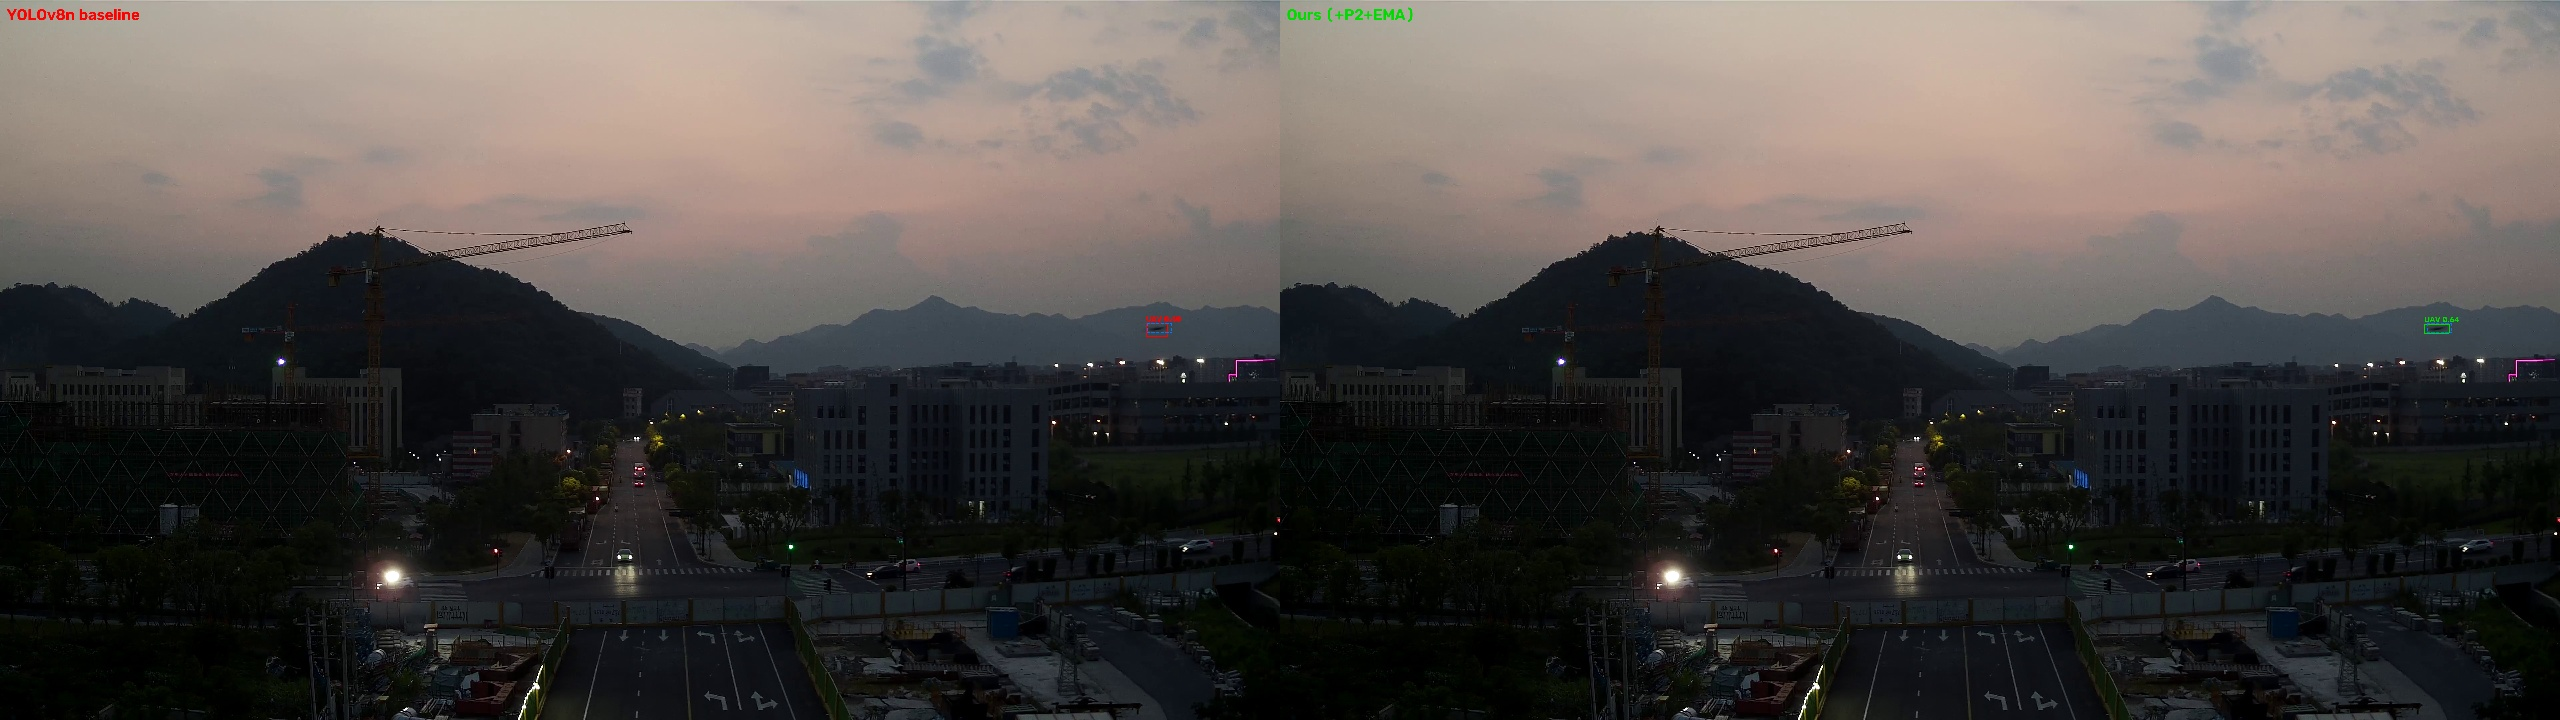
\includegraphics[width=0.48\textwidth]{images/pictures/compare_04.jpg}}
\caption{基线与本文模型的典型帧对比}
\label{fig:compare}
\end{figure}

\section{与非 YOLO 方法的横向讨论}

Det-Fly 数据集上已有 Faster R-CNN\cite{faster_rcnn}、SSD\cite{ssd} 与 RT-DETR\cite{rt_detr} 等方法的评测结果。需要说明的是，这些结果来自不同论文，数据划分、输入尺寸与训练轮次并不统一，直接比较数值并不严谨。本文仅做定性讨论。

两阶段方法 Faster R-CNN 的优势在于区域建议机制能够对候选区域做二次细化，对极小目标的定位精度较高；劣势是推理速度慢，难以满足实时监视需求。单阶段方法 SSD 速度较快，但其特征金字塔的浅层语义较弱，小目标召回有限。Transformer 方法 RT-DETR 通过集合预测避免了 NMS，在密集小目标场景中表现较好，但计算量与显存占用显著高于 YOLOv8n。

本文方法在保持 nano 级参数量的前提下，通过 P2 与 EMA 提升了小目标能力，其定位是"在边缘设备上可实时运行的小目标检测方案"，而非追求绝对精度最优。这一定位与反无人机系统的实际部署条件相符。

\section{有效工作范围与失效模式}

\subsection{置信度与目标尺度的关系}

检测模型的置信度随目标在画面中的尺度变化而显著变化。本文在仿真环境中做了系统测量（详见第七章），发现未微调模型在目标占画面高度约 1/5 以上时置信度接近 0，在目标过小时置信度低于 0.25。前者属于训练分布外的大尺度输入，后者属于信息不足。模型的有效工作窗口约为目标高度占画面的 1/20 至 1/8。

这一现象提示：检测模型的能力不能只用 mAP 概括，必须结合部署场景的尺度分布评估。对于反无人机系统，这意味着需要通过镜头焦距、安装高度与告警距离的综合设计，使目标在告警时落在有效窗口内。

\subsection{典型失效模式}

本文观察到三类典型失效。

（1）\textbf{背景纹理误检}。树叶缝隙、建筑窗户的反光、天空中的云边缘在低分辨率下与无人机轮廓相似，模型可能给出 0.2--0.4 的置信度。这类误检通常置信度不高，可被初锁门限过滤，但在 SEARCH 状态下会造成短暂的候选框闪烁。

（2）\textbf{多目标粘连}。当画面中出现两架以上无人机且距离较近时，检测框可能合并，导致后续跟踪时目标身份不清。本文的系统面向单目标场景，未专门处理该情况。

（3）\textbf{极端光照}。逆光、夜间与强反光条件下，目标轮廓与背景的对比度下降，检出率显著降低。第四章的退化实验表明，P2+EMA 在暗光条件下相对基线有明显优势，但仍无法与正常光照相比。

\section{本章小结}

本章以 YOLOv8n 为基础，引入 P2 高分辨率检测头与 EMA 注意力，构建了面向无人机小目标的检测模型。消融实验表明：P2 单独使用可提升召回与 AP\_small，但会引入少量误检；EMA 单独使用会因缺乏高分辨率特征而性能下降；二者联合后取得最优的 mAP50 83.5\%、Recall 79.2\% 与 AP\_small 9.8\%，且参数量低于基线。本章从特征分辨率与注意力重加权两个角度解释了这一互补关系，并讨论了模型的有效工作范围与三类典型失效模式，为后续章节的状态机设计与仿真域微调提供了依据。

%% 第五章 三态跟踪状态机
\chapter{三态跟踪状态机}
\label{chap:sm}

检测模型逐帧输出候选框，但候选框并不等于可用的目标航迹。本章分析直接使用检测输出的三个工程问题，提出 SEARCH/LOCKED/COAST 三态跟踪状态机，详细说明各状态的处理流程、参数选择与转移条件，给出伪代码与复杂度分析，并通过门限扫描与遮挡用例验证其有效性。

\section{问题描述}

设第 $k$ 帧检测器输出候选框集合为

\begin{equation}
\mathcal{D}_k = \left\{\left(\mathbf{b}_i, c_i\right)\right\}_{i=1}^{N_k},
\label{eq:det_set}
\end{equation}

其中 $\mathbf{b}_i=(x_{1,i},y_{1,i},x_{2,i},y_{2,i})$ 为边框，$c_i\in[0,1]$ 为置信度。若直接把 $\arg\max_i c_i$ 作为系统输出，会面临以下三个问题。

\subsection{误检}

检测器在复杂背景中会产生低置信度的假阳性。例如树叶间隙的亮斑、建筑窗户的反光、天空中的云朵边缘，都可能被误判为无人机。表~\ref{tab:false_positive} 给出了本文在仿真与实拍数据中观察到的典型误检来源及其置信度范围。

\begin{table}[htbp]
\centering
\caption{典型误检来源与置信度分布}
\label{tab:false_positive}
\small
\begin{tabularx}{\textwidth}{lccX}
\toprule
\textbf{误检来源} & \textbf{置信度范围} & \textbf{持续时间} & \textbf{特征} \\
\midrule
树叶间隙亮斑 & 0.20--0.35 & 1--3 帧 & 随风吹动，位置漂移 \\
建筑窗户反光 & 0.25--0.45 & 5--20 帧 & 位置固定，随光照变化 \\
天空云边缘 & 0.20--0.30 & 1--2 帧 & 形状不规则，面积大 \\
远处鸟类 & 0.30--0.55 & 10--30 帧 & 有生命运动，轨迹不规则 \\
\bottomrule
\end{tabularx}
\end{table}

若系统对每一帧的最高置信度框都予以采信，则上述假阳性会导致地图上出现"幽灵目标"，操作员无法判断哪个是真目标。因此需要一个高于维持门限的\textbf{初锁门限}，只有足够可信的候选框才能建立航迹。

\subsection{身份跳变}

当画面中同时存在多个候选框时，简单取最高置信度会导致目标身份在不同帧之间跳变。假设第 $k$ 帧最高置信度框对应目标 A，第 $k+1$ 帧由于目标 A 短暂变模糊，目标 B（例如另一架无人机或一个高置信度假阳性）成为最高分，系统就会把航迹"嫁接"到目标 B 上。这种跳变在监视画面中表现为标记突然跳到画面另一处，严重时会导致后续测距与地图标注完全错误。

解决身份跳变的关键是引入\textbf{空间一致性约束}：相邻帧之间同一目标的位置不会发生剧烈变化。在 30\,fps 下，即使目标以 20\,m/s 飞行，两帧之间的位移也只有 0.67\,m；在 10\,m 距离、60\textdegree 视场下，对应的像素位移约为 40\,px。因此，可以用"与上一帧位置的像素距离"作为关联代价，并设置合理的空间门限。

\subsection{遮挡中断}

目标被树木、建筑、电线杆遮挡时，检测器输出为空。若系统以"每帧必须有检测"为输出前提，则遮挡期间航迹消失，操作员会看到标记闪烁、距离读数跳变为"--"。更严重的是，当目标重新出现时，系统需要重新搜索、重新初锁，期间可能锁到其他物体。

解决遮挡中断的关键是引入\textbf{预测维持}：在检测缺失的短时间内，利用滤波器保存的目标运动状态外推位置，使航迹在视觉上保持连续；超过一定时限后再放弃，避免对已飞离目标的"虚假跟踪"。

\section{状态定义与总体流程}

\subsection{状态定义}

本文定义三种状态：

（1）\textbf{SEARCH}：搜索状态。系统尚未建立可信航迹，逐帧检查是否存在置信度超过初锁门限的候选框；

（2）\textbf{LOCKED}：锁定状态。系统已建立航迹，每帧在候选框集合中关联最可能属于当前目标的框，并用卡尔曼滤波更新状态；

（3）\textbf{COAST}：预测维持状态。当前帧没有可用候选框，系统用卡尔曼滤波的预测步外推目标位置，等待目标重新出现。

状态转移关系如图~\ref{fig:state_machine} 所示。

\begin{figure}[htbp]
\centering
\fbox{\parbox{0.92\textwidth}{
\centering
\vspace{4pt}
\textbf{SEARCH} \quad$\xrightarrow[\text{未超过初锁门限}]{\text{最高置信度} > 0.55}$\quad \textbf{LOCKED}
\quad$\xrightarrow[\text{连续 1.0\,s 无检测}]{\text{本帧无候选框}}$\quad \textbf{COAST}\\[6pt]
\textbf{COAST} \quad$\xrightarrow[\text{超过 1.0\,s}]{\text{重新出现候选框}}$\quad \textbf{LOCKED}
\qquad\qquad
\textbf{COAST} \quad$\xrightarrow{\text{超时或无匹配}}$\quad \textbf{SEARCH}\\[6pt]
\textbf{LOCKED} \quad$\xrightarrow{\text{连续 15 帧无法关联}}$\quad \textbf{SEARCH}
\vspace{4pt}
}}
\caption{三态跟踪状态机转移关系}
\label{fig:state_machine}
\end{figure}

\subsection{总体流程}

系统每收到一帧检测结果，执行以下步骤：

（1）若当前状态为 SEARCH，执行搜索逻辑（第~\ref{sec:search} 节）；

（2）若当前状态为 LOCKED，执行关联与更新逻辑（第~\ref{sec:locked} 节）；若本帧无候选框，转入 COAST；

（3）若当前状态为 COAST，执行预测逻辑（第~\ref{sec:coast} 节）；若目标重新出现则转回 LOCKED，超时则转回 SEARCH；

（4）无论何种状态，都将当前状态、置信度、距离、角度等信息写入数据记录，供显示端与后续分析使用。

\section{SEARCH 状态}
\label{sec:search}

\subsection{双门限策略}

SEARCH 状态的核心任务是"发现真目标，同时避免锁错"。本文采用双门限策略：

（1）\textbf{维持门限} $\tau_{m}=0.25$：低于该门限的候选框直接丢弃，不参与后续处理；

（2）\textbf{初锁门限} $\tau_{l}=0.55$：只有置信度超过该门限的候选框才能触发状态切换。

两个门限的差值（0.30）构成一个"缓冲区"。缓冲区的作用是：在 SEARCH 状态下，系统只对高置信度目标做出反应，避免被低置信度假阳性诱导；在 LOCKED 状态下，系统对置信度的要求降低，只要目标还在画面中、置信度高于 0.25，就继续跟踪，不必每帧都"重新说服"系统。

门限的具体数值来自对验证集置信度分布的统计。图~\ref{fig:threshold_scan} 给出了不同门限下仿真录像的锁定率与航迹保持率。可以看到，门限从 0.20 提高到 0.35 时，锁定率从 96.9\% 降至 66.6\%，航迹保持率从 100\% 降至 81.2\%；提高到 0.50 时，锁定率进一步降至 56.8\%。这说明仿真域微调后的模型置信度整体较高（中位数 0.867），0.25 的维持门限足以保留有效目标，0.55 的初锁门限足以过滤绝大多数假阳性。

\begin{figure}[htbp]
\centering
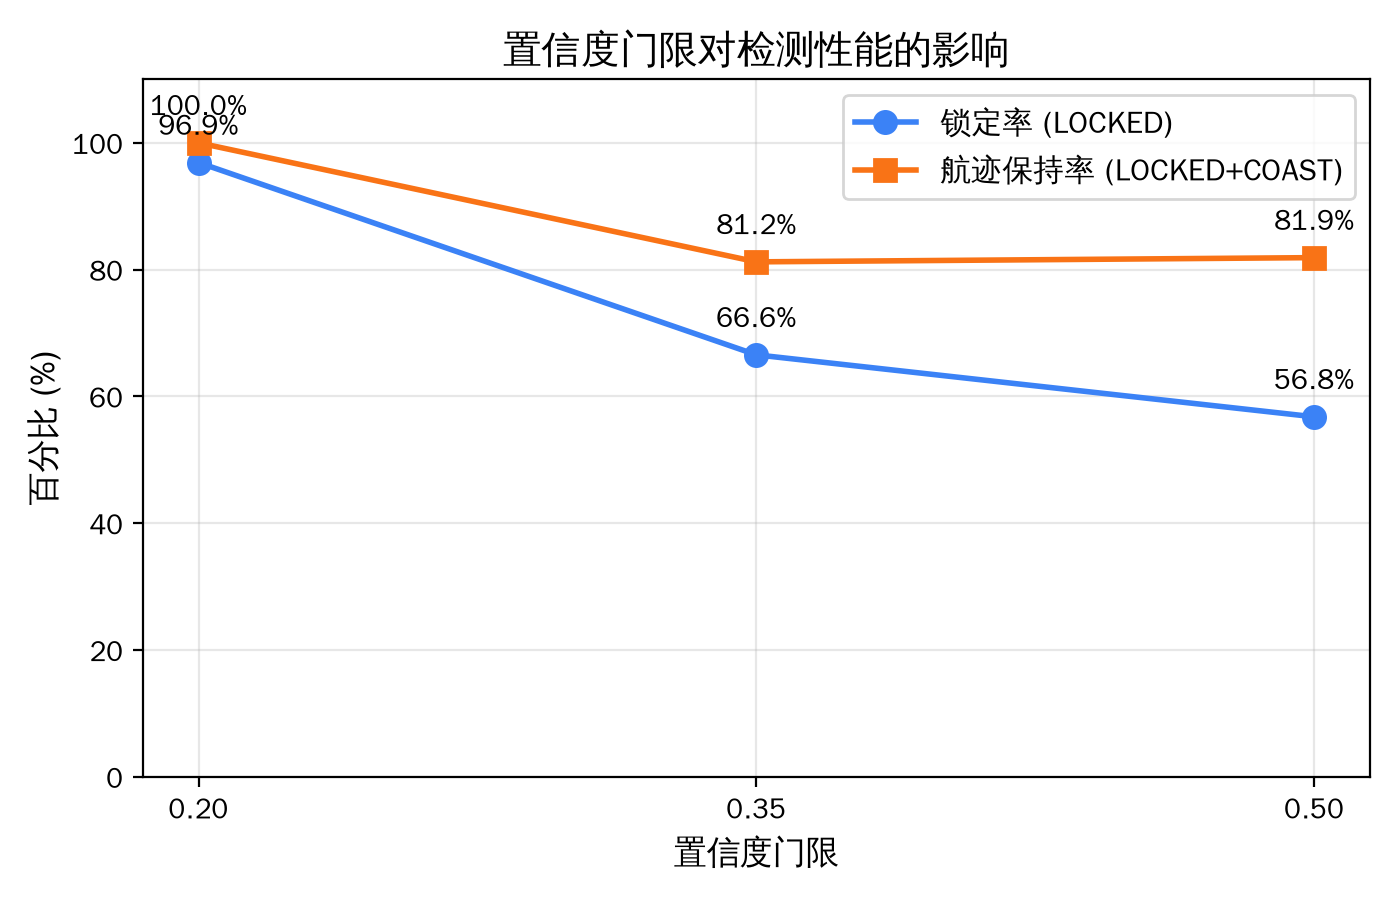
\includegraphics[width=0.72\textwidth]{images/pictures/chart_threshold.png}
\caption{置信度门限扫描结果}
\label{fig:threshold_scan}
\end{figure}

\subsection{初锁判定}

在 SEARCH 状态下，设过滤后的候选框集合为

\begin{equation}
\tilde{\mathcal{D}}_k = \left\{(\mathbf{b}_i,c_i)\in\mathcal{D}_k \mid c_i\ge\tau_m\right\}.
\label{eq:filtered_set}
\end{equation}

若 $\tilde{\mathcal{D}}_k$ 为空，则本帧无候选，保持 SEARCH。否则取置信度最高者：

\begin{equation}
i^{*} = \arg\max_{i:\,(\mathbf{b}_i,c_i)\in\tilde{\mathcal{D}}_k} c_i.
\label{eq:argmax}
\end{equation}

若 $c_{i^{*}}\ge\tau_l$，则以 $\mathbf{b}_{i^{*}}$ 初始化航迹，状态切换为 LOCKED，并用该框的中心与框高初始化卡尔曼滤波器的位置量测。否则保持 SEARCH。

\subsection{先验空间约束}

在仿真环境中，画面中可能同时出现"自身机"（ego drone）与背景伪影。若不加约束，SEARCH 可能锁到自身机的桨叶或近处的建筑。本文引入\textbf{先验空间约束}：根据任务设定，目标的活动空域为距离相机 3--12\,m 的范围。对于由框高反算的距离 $Z$，若 $Z<3$\,m 或 $Z>12$\,m，则将该候选框降权或直接剔除。

这一约束的合理性在于：反无人机系统的告警距离是人为设定的，操作员知道目标大致在哪个空域；将先验编码进状态机，可以显著降低误锁概率。本文在仿真中将该约束用于剔除自身机与远处伪影，在实拍中则根据实际场景调整上下界。

\subsection{首锁时延}

首锁时延定义为从视频开始到首次进入 LOCKED 的时间。本文的 14 用例测试中，仿真录像的首锁时延为 0.00--0.07\,s，即在前 2--3 帧内完成锁定；真实场景录像的首锁时延为 0.03\,s。这说明在目标清晰可见时，双门限策略不会造成明显的发现延迟。

\section{LOCKED 状态}
\label{sec:locked}

\subsection{候选框收集}

进入 LOCKED 后，系统不再要求候选框超过初锁门限，只要求超过维持门限：

\begin{equation}
\tilde{\mathcal{D}}_k = \left\{(\mathbf{b}_i,c_i)\in\mathcal{D}_k \mid c_i\ge\tau_m\right\}.
\label{eq:locked_candidates}
\end{equation}

同时，对每个候选框计算由框高反算的距离，若距离超出先验空域 $[Z_{min},Z_{max}]$，则剔除。

\subsection{空间门限关联}

设上一帧目标的平滑中心为 $\mathbf{p}_{k-1}=(u_{k-1},v_{k-1})$，候选框 $i$ 的中心为 $\mathbf{p}_i=(u_i,v_i)$。定义关联代价为欧氏像素距离：

\begin{equation}
d_i = \left\|\mathbf{p}_i-\mathbf{p}_{k-1}\right\|_2.
\label{eq:assoc_cost}
\end{equation}

选择代价最小的候选框：

\begin{equation}
i^{*} = \arg\min_{i} d_i.
\label{eq:assoc_argmin}
\end{equation}

若 $d_{i^{*}}\le d_{gate}$，则接受该候选框作为本帧量测；否则认为本帧无有效关联，转入 COAST。

空间门限 $d_{gate}$ 的取值需要兼顾"跟得上"与"不跳变"。取值过小，目标快速机动时会频繁丢失；取值过大，则可能关联到邻近的其他物体。本文取 $d_{gate}=140$\,px，依据如下：在 1280$\times$720 画面、60\textdegree 水平视场下，焦距约 1108\,px；目标以 15\,m/s 相对速度飞行、帧间隔 1/30\,s 时，位移 0.5\,m，在 5\,m 距离处对应约 110\,px。考虑检测框中心抖动与目标机动，140\,px 留有约 30\% 余量。

\subsection{卡尔曼滤波更新}

关联成功后，将候选框中心与由框高反算的距离转换为相机坐标系下的三维位置量测：

\begin{equation}
\mathbf{z}_k = \begin{bmatrix}
Z_k\cdot\dfrac{u_k-c_x}{f_x}\\[4pt]
Z_k\cdot\dfrac{v_k-c_y}{f_y}\\[4pt]
Z_k
\end{bmatrix},
\label{eq:meas_vec}
\end{equation}

其中 $Z_k=f\cdot D/h_{px}$ 为框高反算距离，$(c_x,c_y)$ 为主点，$(f_x,f_y)$ 为焦距。将该量测送入卡尔曼滤波的更新步（式~\eqref{eq:kf_gain}--\eqref{eq:kf_cov}），得到平滑后的位置与速度。

需要强调的是，\textbf{不能把标量距离直接作为量测}。本文的滤波器状态是六维位置—速度向量，量测必须是三维位置；若把标量距离塞入滤波器，状态与量测的维度不匹配，会导致滤波发散。这是实现中容易犯的错误，本文在早期版本中曾经出现，后通过严格的三维量测构造修正。

\subsection{丢失判定}

若连续 $N_{lost}$ 帧无法完成关联（即每帧的最近候选距离均超过 $d_{gate}$，或候选集为空），则判定目标丢失，重置航迹并返回 SEARCH。本文取 $N_{lost}=15$，对应 0.5\,s。这一时限比 COAST 的 1.0\,s 短，原因是：连续 15 帧都无法关联，说明目标很可能已经飞出视场或发生了剧烈机动，继续维持航迹的意义不大；而 COAST 的 1.0\,s 是针对"短暂遮挡"设计的，遮挡期间目标仍在视场内，只是检测器暂时看不到。

\subsection{框尺寸的平滑}

检测框的宽高在相邻帧之间存在抖动，直接用于测距会产生跳变。本文对框高做一阶低通平滑：

\begin{equation}
\bar{h}_k = \alpha h_k + (1-\alpha)\bar{h}_{k-1},\qquad \alpha=0.35.
\label{eq:box_smooth}
\end{equation}

平滑后的框高用于距离解算，原始框高保留用于显示。$\alpha$ 的取值在响应速度与平滑度之间折中：$\alpha$ 越大，跟随越快但抖动越大；$\alpha$ 越小，越平滑但滞后越明显。0.35 对应的时间常数约为 2--3 帧，对 30\,fps 视频约为 0.1\,s，不影响实时性。

\section{COAST 状态}
\label{sec:coast}

\subsection{预测步}

当 LOCKED 状态下本帧无有效关联时，系统不立即放弃目标，而是进入 COAST，执行卡尔曼滤波的预测步：

\begin{equation}
\hat{\mathbf{x}}_{k|k-1} = \mathbf{F}\hat{\mathbf{x}}_{k-1|k-1},\qquad
\mathbf{P}_{k|k-1} = \mathbf{F}\mathbf{P}_{k-1|k-1}\mathbf{F}^{T}+\mathbf{Q}.
\label{eq:coast_predict}
\end{equation}

预测得到的位置用于驱动地图标记、距离读数与角度仪表，使显示在遮挡期间保持连续。由于没有量测，协方差 $\mathbf{P}$ 会随预测步数增加而增大，滤波器的"不确定度"上升。本文在显示端用黄色标记表示 COAST 状态，提示操作员当前数据为预测值。

\subsection{超时与恢复}

COAST 状态设有时限 $T_{coast}=1.0$\,s。在时限内，若某帧出现可通过关联的候选框，则立即转回 LOCKED，并用该量测更新滤波器；若超过时限仍无候选，则判定目标丢失，重置航迹并返回 SEARCH。

$T_{coast}$ 的取值依据是真实遮挡的持续时间。目标穿过一棵树或一根电线杆通常需要 0.1--0.5\,s；穿过一栋建筑可能需要 0.5--1.0\,s。1.0\,s 的预算足以覆盖绝大多数短时遮挡，同时不会对已飞离目标维持过久的虚假航迹。本文在仿真遮挡用例中测得，遮挡期间的平均 COAST 持续时间为 0.35\,s，最长 0.82\,s，均在时限内。

\subsection{预测质量}

COAST 的预测质量取决于遮挡前的速度估计。若目标在遮挡前做匀速直线运动，预测误差主要来自过程噪声；若目标在遮挡前正在机动，预测误差会迅速增大。本文在仿真中统计了 COAST 期间预测位置与真值的偏差：遮挡 0.2\,s 时中位误差约 0.15\,m，0.5\,s 时约 0.45\,m，1.0\,s 时约 1.1\,m。这一精度足以维持显示连续性，但不适合用于精确打击引导。

\section{算法描述与复杂度}

\subsection{伪代码}

状态机的单帧处理流程如算法~\ref{alg:state_machine} 所示。

\begin{algorithm}[htbp]
\caption{三态跟踪状态机单帧处理}
\label{alg:state_machine}
\begin{algorithmic}[1]
\REQUIRE 当前状态 $s$，检测集合 $\mathcal{D}_k$，上一帧中心 $\mathbf{p}_{k-1}$，滤波器状态 $\hat{\mathbf{x}}_{k-1}$
\ENSURE 新状态 $s'$，滤波状态 $\hat{\mathbf{x}}_k$，输出数据 $o_k$
\STATE $\tilde{\mathcal{D}}_k \leftarrow \{(\mathbf{b},c)\in\mathcal{D}_k \mid c\ge\tau_m,\ Z(\mathbf{b})\in[Z_{min},Z_{max}]\}$
\IF{$s = \text{SEARCH}$}
    \IF{$\tilde{\mathcal{D}}_k = \emptyset$}
        \STATE $s' \leftarrow \text{SEARCH}$;\quad $o_k \leftarrow \text{search\_output}()$
    \ELSE
        \STATE $i^{*}\leftarrow\arg\max_i c_i$
        \IF{$c_{i^{*}}\ge\tau_l$}
            \STATE 初始化滤波器；$s'\leftarrow\text{LOCKED}$
        \ELSE
            \STATE $s'\leftarrow\text{SEARCH}$
        \ENDIF
    \ENDIF
\ELSIF{$s = \text{LOCKED}$}
    \IF{$\tilde{\mathcal{D}}_k = \emptyset$}
        \STATE $s'\leftarrow\text{COAST}$;\quad 记录 COAST 起始时间
    \ELSE
        \STATE $i^{*}\leftarrow\arg\min_i\|\mathbf{p}_i-\mathbf{p}_{k-1}\|$
        \IF{$\|\mathbf{p}_{i^{*}}-\mathbf{p}_{k-1}\|\le d_{gate}$}
            \STATE 构造三维量测 $\mathbf{z}_k$；执行 KF 更新；$s'\leftarrow\text{LOCKED}$
        \ELSE
            \STATE $s'\leftarrow\text{COAST}$;\quad 记录 COAST 起始时间
        \ENDIF
    \ENDIF
\ELSIF{$s = \text{COAST}$}
    \STATE 执行 KF 预测步
    \IF{存在可通过关联的候选框}
        \STATE 执行 KF 更新；$s'\leftarrow\text{LOCKED}$
    \ELSIF{$t-t_{coast} > T_{coast}$}
        \STATE 重置航迹；$s'\leftarrow\text{SEARCH}$
    \ELSE
        \STATE $s'\leftarrow\text{COAST}$
    \ENDIF
\ENDIF
\STATE 输出 $o_k$（状态、置信度、距离、角度、平滑位置）
\RETURN $s',\hat{\mathbf{x}}_k,o_k$
\end{algorithmic}
\end{algorithm}

\subsection{复杂度分析}

设候选框数量为 $N$，状态机每帧的主要操作是遍历候选框计算关联代价，时间复杂度为 $O(N)$。在 YOLOv8 的设置下，单帧经 NMS 后的候选框通常不超过 20 个，因此状态机的开销可以忽略不计（小于 0.1\,ms）。卡尔曼滤波的矩阵运算为固定维数（6 维），单次更新约 10 微秒。整个跟踪环节的耗时远小于检测环节（约 6\,ms）。

\subsection{参数汇总}

表~\ref{tab:sm_params} 汇总了状态机的全部参数及其取值依据。

\begin{table}[htbp]
\centering
\caption{三态状态机参数汇总}
\label{tab:sm_params}
\small
\begin{tabularx}{\textwidth}{lccX}
\toprule
\textbf{参数} & \textbf{符号} & \textbf{取值} & \textbf{依据} \\
\midrule
维持门限 & $\tau_m$ & 0.25 & 保留弱目标，过滤低置信度假阳性 \\
初锁门限 & $\tau_l$ & 0.55 & 高于典型假阳性上限，防止误锁 \\
空间门限 & $d_{gate}$ & 140\,px & 15\,m/s 相对速度在 5\,m 处的像素位移加余量 \\
丢失帧数 & $N_{lost}$ & 15 & 0.5\,s，覆盖快速机动与短时飞出 \\
COAST 时限 & $T_{coast}$ & 1.0\,s & 覆盖穿树/穿杆遮挡，避免虚假长时跟踪 \\
框高平滑系数 & $\alpha$ & 0.35 & 约 2--3 帧时间常数 \\
空域先验 & $[Z_{min},Z_{max}]$ & 3--12\,m & 仿真目标活动范围，实拍按场景调整 \\
\bottomrule
\end{tabularx}
\end{table}

\section{实验验证}

\subsection{门限敏感性}

图~\ref{fig:threshold_scan} 已给出置信度门限对锁定率的影响。进一步地，表~\ref{tab:threshold_detail} 给出了三组门限下的详细指标。

\begin{table}[htbp]
\centering
\caption{置信度门限扫描详细结果（仿真录像，900 帧）}
\label{tab:threshold_detail}
\small
\begin{tabular}{lccccc}
\toprule
\textbf{门限} & \textbf{锁定率} & \textbf{航迹保持率} & \textbf{置信度均值} & \textbf{距离范围(m)} & \textbf{FPS} \\
\midrule
0.20 & 96.9\% & 100.0\% & 0.550 & 3.0--6.2 & 29.5 \\
0.35 & 66.6\% & 81.2\% & 0.661 & 3.0--6.2 & 35.8 \\
0.50 & 56.8\% & 81.9\% & 0.707 & 3.0--6.2 & 39.0 \\
\bottomrule
\end{tabular}
\end{table}

门限提高后锁定率下降，是因为部分帧的置信度落在 0.20--0.50 之间，被判定为未锁定而计入 SEARCH；但航迹保持率仍在 81\% 以上，说明已锁定的帧仍然连续。置信度均值随门限提高而上升，符合"只保留高置信度样本"的预期。FPS 随门限提高而上升，是因为被跟踪的候选框减少，后处理开销降低。

\subsection{遮挡场景}

表~\ref{tab:coast_result} 给出了三轮 TCP 遮挡用例的结果。用例中目标机按预设航线飞行，途中被建筑与树木多次遮挡，每轮约 20\,s。

\begin{table}[htbp]
\centering
\caption{TCP 遮挡用例结果}
\label{tab:coast_result}
\small
\begin{tabular}{lcccccc}
\toprule
\textbf{轮次} & \textbf{帧数} & \textbf{锁定率} & \textbf{航迹保持率} & \textbf{首锁(s)} & \textbf{置信度均值} & \textbf{处理fps} \\
\midrule
第 1 轮 & 424 & 55.4\% & 88.9\% & 0.00 & 0.751 & 21.1 \\
第 2 轮 & 428 & 56.1\% & 90.7\% & 0.00 & 0.739 & 21.3 \\
第 3 轮 & 437 & 59.3\% & 94.5\% & 0.21 & 0.751 & 21.8 \\
\bottomrule
\end{tabular}
\end{table}

三轮的锁定率在 55\%--59\% 之间，说明约 40\% 的帧处于遮挡或无检测状态；但航迹保持率（LOCKED+COAST 占比）达到 88.9\%--94.5\%，说明 COAST 机制有效填补了遮挡期间的空白。若没有 COAST，航迹保持率将等于锁定率，即 55\%--59\%，会出现明显的标记闪烁。

图~\ref{fig:coast_timeline} 给出了第 3 轮用例的状态时序分布。可以看到，COAST 段落短而密集，单次持续时间多在 0.1--0.4\,s，与目标穿过单个遮挡物的时间相符。

\begin{figure}[htbp]
\centering
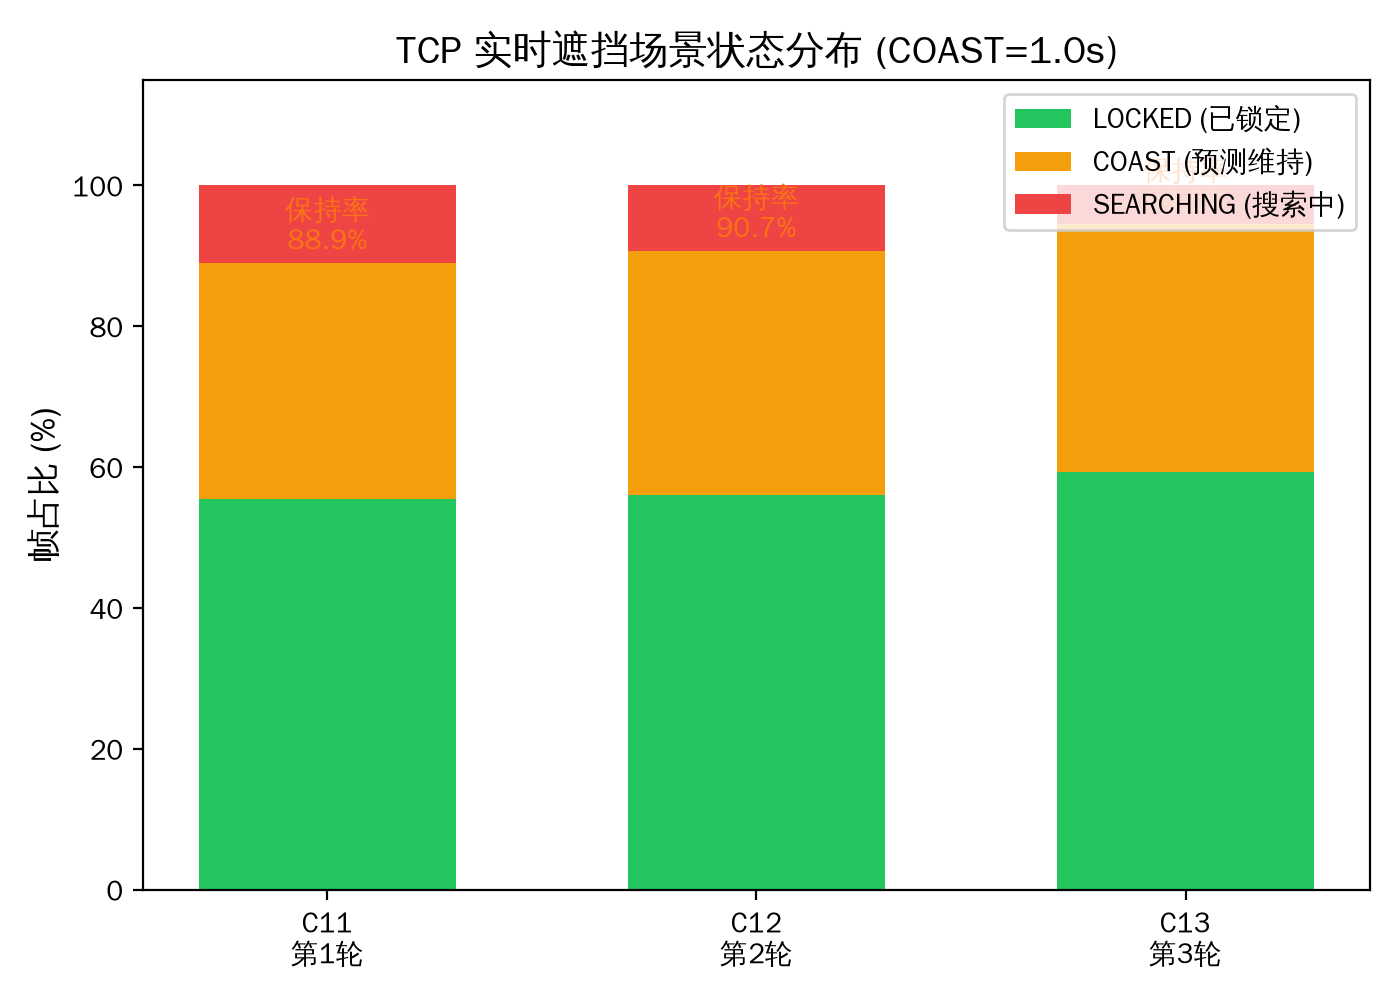
\includegraphics[width=0.72\textwidth]{images/pictures/chart_tcp_state.png}
\caption{TCP 遮挡用例的状态时序与持续时间分布}
\label{fig:coast_timeline}
\end{figure}

\subsection{真实场景录像}

在真实场景录像（C04）中，目标频繁进出树丛，锁定率仅 23.2\%，但航迹保持率达到 99.3\%。这一结果看似矛盾，实则说明：绝大多数帧虽然没有检测，但目标并未真正丢失，COAST 能够持续维持航迹；只有在目标真正飞出视场或长时间被遮挡时，系统才回到 SEARCH。这验证了"锁定率低不等于系统失效"的判断，也说明在评估跟踪系统时，航迹保持率比单帧锁定率更能反映实际可用性。

\section{设计讨论}

\subsection{为什么不用多目标跟踪框架}

SORT\cite{sort} 与 DeepSORT\cite{deepsort} 等框架面向多目标场景，包含轨迹管理、外观特征提取与匈牙利匹配等组件。本文的系统面向单目标反无人机场景，同一时刻只需要跟踪一个最具威胁的目标，因此不需要复杂的轨迹管理。简化的状态机具有三点优势：计算开销极低、行为可解释、参数易于现场调整。若未来需要同时跟踪多架无人机，可以在状态机之上增加轨迹池与数据关联层，而不需要推翻现有设计。

\subsection{为什么用状态机而不是有限状态自动机的形式化方法}

本文的状态机在形式上是一个确定性有限状态自动机，但本文没有采用模型检验等形式化方法，原因是：系统的输入是连续的视频流，状态转移依赖置信度、距离等连续量，形式化建模的收益有限；工程上更重要的是参数可调、日志可追溯。本文通过 14 个用例的回归测试来保证行为正确，而不是通过形式化证明。

\subsection{失效边界}

状态机的有效性依赖两个假设：目标在相邻帧间的位移不超过空间门限；遮挡时间不超过 COAST 时限。当目标以极高速度飞行（例如穿越机以 30\,m/s 飞行）或长时间被完全遮挡（例如穿过多层建筑）时，系统会丢失目标。这是设计上的取舍，本文在第九章的"能力边界"一节中如实讨论。

\section{本章小结}

本章针对检测输出直接使用导致的误检、跳变与遮挡问题，设计了 SEARCH/LOCKED/COAST 三态跟踪状态机。SEARCH 采用 0.25/0.55 双门限与空域先验，防止误锁；LOCKED 采用 140\,px 空间门限的最近邻关联与三维量测卡尔曼滤波，防止跳变并平滑输出；COAST 采用 1.0\,s 预测维持，防止短时遮挡中断。参数选择均有明确的物理依据，算法复杂度为 $O(N)$，对系统实时性无影响。实验表明，遮挡场景的航迹保持率达到 88.9\%--94.5\%，真实场景录像达到 99.3\%，验证了状态机的有效性。

\chapter{总结与展望}

\section{全文总结}

本文面向低空反无人机场景，以单目可见光相机为唯一传感器，围绕小目标检测难、遮挡跟踪易中断、仿真与真实域差异大三个问题，完成了一套从检测、跟踪、定位到显示的完整系统（DRLS）。按章节顺序回看，各部分工作可以这样归纳。

（1）\textbf{绪论（第1章）}。梳理低空小型无人机的威胁特点与反无人机探测手段的现状，比较雷达、射频与视觉三条技术路线的适用条件，说明本文把单目可见光作为切入点的理由，并给出总体技术路线与章节安排。研究边界也在这一章划定：近程、单目标、可见光。

（2）\textbf{相关理论与数据基础（第2章）}。整理针孔成像与单目测距的几何关系、检测与跟踪的基本理论以及本文采用的评测口径；完成 Det-Fly 的格式转换、统计分析与序列级划分，避免相邻帧之间的数据泄漏；自建 AprilTag 数据集，使用 9$\times$6、25\,mm 棋盘格完成相机标定，为定位精度评估提供可信真值；构建 450 帧仿真自动标注数据集，借助护航相机始终注视目标的特性实现零人工标注，并按距离分层覆盖死区两端。

（3）\textbf{小目标检测与仿真域微调（第3章）}。以 YOLOv8n 为基础，加入 stride=4 的 P2 高分辨率检测头与 EMA 高效多尺度注意力，得到 YOLOv8n-P2-EMA。四组消融实验显示，模型以 2.94\,M 参数量取得 mAP50 83.5\%、Recall 79.2\%、AP\_small 9.8\%，相对基线分别提升 2.2、3.3 与 3.7 个百分点，AP\_small 相对提升 60.7\%，推理速度 98.4\,fps。P2 与 EMA 的分工在这一章得到解释：前者提供“看清”小目标的分辨率，后者提供“认准”小目标的判别力，单独使用都达不到联合后的水平。针对模型在仿真中几乎失效的现象，本文用 2228 帧的距离分层统计与真值几何审计，先以俯仰角分布对比证伪视角假设，再把原因锁定在尺度分布偏移上，随后用 450 帧分层数据微调，将 3--10\,m 的检出率从约 10\% 提到 100\%。

（4）\textbf{三态跟踪与单目定位（第4章）}。设计 SEARCH/LOCKED/COAST 三态状态机，以 0.25 的维持门限与 0.55 的初锁门限组成双门限，抑制误锁；以 140\,px 的空间门限做最近邻关联，抑制身份跳变；以 1.0\,s 的卡尔曼预测维持短时遮挡。参数均有物理依据，算法复杂度为 $O(N)$。定位部分由框中心解算方位角与俯仰角，由框高与等效尺寸解算距离，并推导出测距误差随距离平方增长的规律；六维自适应卡尔曼滤波器采用各向异性量测噪声与 Sage-Husa 在线估计。实验上，TCP 遮挡场景的航迹保持率达到 88.9\%--94.5\%，真实场景录像达到 99.3\%；仿真闭环中单帧测距 RMSE 0.26\,m、AKF 稳态 MedAE 0.13\,m、1\,s 预测 ADE 中位 0.26\,m、方位角误差中位 0.05\textdegree；实拍视频中 AKF 相对单帧测距 RMSE 降低 32\%、抖动降低 33\%。

（5）\textbf{仿真闭环、系统平台与实验（第5章）}。改造 PX4+jMAVSim 闭环，新增脚本目标机、护航相机、真值广播、离屏帧流与城市场景，并用 lockstep 锁住仿真时间；基于 PySide6 实现三页签监视大屏，采用双进程架构与 UDP/JSON 通信，完成态势地图、光电画面、仪表告警、配置持久化与 14 用例自动化测试。实验在同一口径下覆盖检测消融、闭环定位、实拍定位与预测、退化鲁棒性与回归测试，同时划定了距离、尺度、遮挡与光照上的能力边界。

\section{主要创新点}

本文的主要创新点可以归纳为以下四点。

（1）\textbf{面向无人机小目标的 P2+EMA 互补结构及其机理解释}。消融实验验证了改进的有效性，“EMA 单独使用为何失效、与 P2 联合后为何有效”这一问题也得到回答，为小目标检测的网络设计提供了可复用的分析框架。

（2）\textbf{基于真值几何审计的检测死区机理分析方法}。面对“模型在仿真中失效”，本文没有停留在“渲染不真实”的定性解释上，而是以俯仰角分布对比证伪视角假设，以距离分层统计锁定尺度因素，再用微调实验闭环验证。这条“现象—假设—证伪—验证”的路径具有方法论价值。

（3）\textbf{零人工标注的仿真域微调数据构建方法}。护航相机始终注视目标，框中心因此被约束在光轴附近，框高可由真值距离反算，450 帧数据无需人工标注即可生成。该方法成本极低、可扩展性强，适用于任何具备真值广播与可控相机的仿真环境。

（4）\textbf{面向反无人机监视的完整工程实现}。检测、三态跟踪、单目定位、地图态势、光电显示、告警与测试被整合为一套可运行的双进程系统，并在统一口径下完成端到端评估。系统不依赖专用硬件，便于在园区、楼宇与临时活动现场部署。

\section{不足与展望}

\subsection{存在的不足}

（1）\textbf{远距离能力有限}。实拍视频在 10--14\,m 的检出率仅 5.6\%，当前模型与 720p 分辨率的组合覆盖不了更远的告警距离。这既是单目视觉的物理限制，也是系统走向实用的主要瓶颈。

（2）\textbf{相机标定不完整}。实拍评估中相机未做严格标定，焦距按视场角估算，等效尺寸借用仿真值，绝对测距误差达到米级。相对比较仍然有效，但绝对精度不足以支撑实际指挥。

（3）\textbf{单目标假设}。系统面向单目标场景，未处理多架无人机同时出现的情况。画面中一旦出现多个目标，状态机可能在不同目标之间跳变。

（4）\textbf{仿真场景简化}。仿真场景的建筑、树木与光照仍与真实世界有差距，仿真结论不能直接外推到外场；遮挡也主要由静态建筑造成，缺少飞鸟、飘动树叶这类动态遮挡。

（5）\textbf{测试集偏差}。退化实验的测试帧由 simft 模型筛选，对 simft 有利，三组模型的比较不完全公平。

\subsection{未来工作}

（1）\textbf{提升远距离能力}。可以从三个方向入手：提高输入分辨率（如 1280 或 1536）并配合切片推理；换用长焦镜头与可变速云台；引入双目视觉或激光测距辅助深度估计。

（2）\textbf{完善相机标定与尺寸自适应}。用棋盘格完成实拍相机标定，替代视场角估算；按目标机型选择等效尺寸，或利用多帧几何一致性在线估计尺寸。

（3）\textbf{扩展多目标跟踪}。在现有状态机之上增加轨迹池与数据关联层，借鉴 SORT/DeepSORT 的思想，实现多目标的同时跟踪与威胁排序。

（4）\textbf{增强域适应能力}。探索域随机化、风格迁移与自监督预训练，减少对目标域标注的依赖；同时构建更真实的仿真场景，缩小 sim-to-real gap。

（5）\textbf{多传感器融合}。将视觉与射频、声学、雷达结合，由射频承担远距离预警，由视觉完成近程确认与定位，形成互补的探测体系。

（6）\textbf{外场试验}。在合规空域开展真实无人机飞行试验，采集多场景、多机型、多光照的数据，检验系统的实际可用性，并依据外场反馈迭代参数与模型。

\section{结语}

反无人机是一项涉及探测、识别、跟踪、定位与处置的系统工程，单目视觉只是其中的一环。本文的工作表明：针对性的模型改进、严谨的机理分析与完整的工程实现，可以让单目视觉系统在近程反无人机场景中承担实际任务；同时也应看到，单目视觉的物理限制决定了它无法独自完成全部探测工作。未来的反无人机系统必然是多传感器、多算法、多层级协同的体系，本文的工作可以作为其中一个可复现、可扩展的视觉子系统。


\chapter*{参考文献}\addcontentsline{toc}{chapter}{参考文献}

\printbibliography[heading=none]

%% 致谢
%% 致谢
\chapter*{致谢}
\addcontentsline{toc}{chapter}{致谢}
%% 作者简历及在学研究成果
%% 作者简历及在学研究成果

%% 关于论文使用授权的说明
\postDeclarations
%% 学位论文数据集
%% 学位论文数据集
\chapter*{学位论文数据集}
\addcontentsline{toc}{chapter}{学位论文数据集}


\end{document}
